% Options for packages loaded elsewhere
\PassOptionsToPackage{unicode}{hyperref}
\PassOptionsToPackage{hyphens}{url}
%
\documentclass[
  a4paper,
]{scrbook}

\usepackage{amsmath,amssymb}
\usepackage{iftex}
\ifPDFTeX
  \usepackage[T1]{fontenc}
  \usepackage[utf8]{inputenc}
  \usepackage{textcomp} % provide euro and other symbols
\else % if luatex or xetex
  \usepackage{unicode-math}
  \defaultfontfeatures{Scale=MatchLowercase}
  \defaultfontfeatures[\rmfamily]{Ligatures=TeX,Scale=1}
\fi
\usepackage{lmodern}
\ifPDFTeX\else  
    % xetex/luatex font selection
  \setmainfont[]{Latin Modern Roman}
  \setsansfont[]{Latin Modern Roman}
\fi
% Use upquote if available, for straight quotes in verbatim environments
\IfFileExists{upquote.sty}{\usepackage{upquote}}{}
\IfFileExists{microtype.sty}{% use microtype if available
  \usepackage[]{microtype}
  \UseMicrotypeSet[protrusion]{basicmath} % disable protrusion for tt fonts
}{}
\makeatletter
\@ifundefined{KOMAClassName}{% if non-KOMA class
  \IfFileExists{parskip.sty}{%
    \usepackage{parskip}
  }{% else
    \setlength{\parindent}{0pt}
    \setlength{\parskip}{6pt plus 2pt minus 1pt}}
}{% if KOMA class
  \KOMAoptions{parskip=half}}
\makeatother
\usepackage{xcolor}
\setlength{\emergencystretch}{3em} % prevent overfull lines
\setcounter{secnumdepth}{5}
% Make \paragraph and \subparagraph free-standing
\ifx\paragraph\undefined\else
  \let\oldparagraph\paragraph
  \renewcommand{\paragraph}[1]{\oldparagraph{#1}\mbox{}}
\fi
\ifx\subparagraph\undefined\else
  \let\oldsubparagraph\subparagraph
  \renewcommand{\subparagraph}[1]{\oldsubparagraph{#1}\mbox{}}
\fi


\providecommand{\tightlist}{%
  \setlength{\itemsep}{0pt}\setlength{\parskip}{0pt}}\usepackage{longtable,booktabs,array}
\usepackage{calc} % for calculating minipage widths
% Correct order of tables after \paragraph or \subparagraph
\usepackage{etoolbox}
\makeatletter
\patchcmd\longtable{\par}{\if@noskipsec\mbox{}\fi\par}{}{}
\makeatother
% Allow footnotes in longtable head/foot
\IfFileExists{footnotehyper.sty}{\usepackage{footnotehyper}}{\usepackage{footnote}}
\makesavenoteenv{longtable}
\usepackage{graphicx}
\makeatletter
\def\maxwidth{\ifdim\Gin@nat@width>\linewidth\linewidth\else\Gin@nat@width\fi}
\def\maxheight{\ifdim\Gin@nat@height>\textheight\textheight\else\Gin@nat@height\fi}
\makeatother
% Scale images if necessary, so that they will not overflow the page
% margins by default, and it is still possible to overwrite the defaults
% using explicit options in \includegraphics[width, height, ...]{}
\setkeys{Gin}{width=\maxwidth,height=\maxheight,keepaspectratio}
% Set default figure placement to htbp
\makeatletter
\def\fps@figure{htbp}
\makeatother

\usepackage{booktabs}
\usepackage{longtable}
\usepackage{array}
\usepackage{multirow}
\usepackage{wrapfig}
\usepackage{float}
\usepackage{colortbl}
\usepackage{pdflscape}
\usepackage{tabu}
\usepackage{threeparttable}
\usepackage{threeparttablex}
\usepackage[normalem]{ulem}
\usepackage{makecell}
\usepackage{xcolor}
\usepackage{titling}
\setlength{\droptitle}{-2cm}
\preauthor{
  \begin{center}
  \Large
  \vspace{10mm}
  by

  \vspace{20mm}
}
\postauthor{
  \end{center}
  \vfill
}

\predate{
  \begin{center}
  A thesis 
  submitted in fulfilment of the \\
  requirements of the degree of \\
  Doctor of Philosophy in Physics\\               % Degree
  School of Physical and Chemical Sciences\\          % Department
  Te Herenga Waka - Victoria University of Wellington\\                       % University 
  \vspace{5mm}
}
\postdate{
  \\
  
\includegraphics[width=3in,height=1.5in]{figures/VUW-logo.png}\\
  \end{center}
  }
\makeatletter
\makeatother
\makeatletter
\@ifpackageloaded{bookmark}{}{\usepackage{bookmark}}
\makeatother
\makeatletter
\@ifpackageloaded{caption}{}{\usepackage{caption}}
\AtBeginDocument{%
\ifdefined\contentsname
  \renewcommand*\contentsname{Table of contents}
\else
  \newcommand\contentsname{Table of contents}
\fi
\ifdefined\listfigurename
  \renewcommand*\listfigurename{List of Figures}
\else
  \newcommand\listfigurename{List of Figures}
\fi
\ifdefined\listtablename
  \renewcommand*\listtablename{List of Tables}
\else
  \newcommand\listtablename{List of Tables}
\fi
\ifdefined\figurename
  \renewcommand*\figurename{Figure}
\else
  \newcommand\figurename{Figure}
\fi
\ifdefined\tablename
  \renewcommand*\tablename{Table}
\else
  \newcommand\tablename{Table}
\fi
}
\@ifpackageloaded{float}{}{\usepackage{float}}
\floatstyle{ruled}
\@ifundefined{c@chapter}{\newfloat{codelisting}{h}{lop}}{\newfloat{codelisting}{h}{lop}[chapter]}
\floatname{codelisting}{Listing}
\newcommand*\listoflistings{\listof{codelisting}{List of Listings}}
\makeatother
\makeatletter
\@ifpackageloaded{caption}{}{\usepackage{caption}}
\@ifpackageloaded{subcaption}{}{\usepackage{subcaption}}
\makeatother
\makeatletter
\@ifpackageloaded{tcolorbox}{}{\usepackage[skins,breakable]{tcolorbox}}
\makeatother
\makeatletter
\@ifundefined{shadecolor}{\definecolor{shadecolor}{rgb}{.97, .97, .97}}
\makeatother
\makeatletter
\makeatother
\makeatletter
\makeatother
\ifLuaTeX
  \usepackage{selnolig}  % disable illegal ligatures
\fi
\usepackage[citestyle = ieee,urldate = iso8601]{biblatex}
\addbibresource{references.bib}
\IfFileExists{bookmark.sty}{\usepackage{bookmark}}{\usepackage{hyperref}}
\IfFileExists{xurl.sty}{\usepackage{xurl}}{} % add URL line breaks if available
\urlstyle{same} % disable monospaced font for URLs
\hypersetup{
  pdftitle={Volatile Organic Compound Detection Using Insect Odorant-Receptor Functionalised Field-Effect Transistors},
  pdfauthor={Eddyn Oswald Perkins Treacher},
  hidelinks,
  pdfcreator={LaTeX via pandoc}}

\title{Volatile Organic Compound Detection Using Insect Odorant-Receptor
Functionalised Field-Effect Transistors}
\author{Eddyn Oswald Perkins Treacher}
\date{Apr 2024}

\begin{document}
\frontmatter
\maketitle
\ifdefined\Shaded\renewenvironment{Shaded}{\begin{tcolorbox}[frame hidden, sharp corners, breakable, borderline west={3pt}{0pt}{shadecolor}, interior hidden, enhanced, boxrule=0pt]}{\end{tcolorbox}}\fi

\renewcommand*\contentsname{Table of contents}
{
\setcounter{tocdepth}{2}
\tableofcontents
}
\mainmatter
\bookmarksetup{startatroot}

\hypertarget{acknowledgements}{%
\chapter*{Acknowledgements}\label{acknowledgements}}
\addcontentsline{toc}{chapter}{Acknowledgements}

\markboth{Acknowledgements}{Acknowledgements}

\begin{verbatim}
69450
\end{verbatim}

Rifat, Alex - vapour sensor Erica Cassie - FET sensing setup Rob Keyzers
and Jennie Ramirez-Garcia - NMR spectra Patricia Hunt - Computational
chemistry

\bookmarksetup{startatroot}

\hypertarget{biosensing-with-insect-odorant-receptor-functionalised-carbon-nanotube-devices}{%
\chapter{Biosensing with Insect Odorant-Receptor Functionalised Carbon
Nanotube
Devices}\label{biosensing-with-insect-odorant-receptor-functionalised-carbon-nanotube-devices}}

\hypertarget{introduction}{%
\section{Introduction}\label{introduction}}

To test devices with the new vapour delivery system, it was important to
first ensure the functionalised devices worked consistently as
biosensors in the existing aqueous sensing setup.

\hypertarget{sec-aqueous-sensing-EtHex}{%
\section{Aqueous Sensing of Ethyl Hexanoate with OR22a-functionalised
Carbon Nanotube Transistor}\label{sec-aqueous-sensing-EtHex}}

\hypertarget{sec-working-PBASE-functionalisation}{%
\subsection{OR Nanodisc
Functionalisation}\label{sec-working-PBASE-functionalisation}}

A carbon nanotube network field-effect transistor device, fabricated
using post-June 2023 methods as described in \textbf{?@sec-fabrication},
was functionalised with OR22a nanodiscs. The network used for the device
was deposited using the steam-assisted surfactant method, and the device
was encapsulated with AZ\(^\circledR\) 1518 using the post-Jan 2023
photolithography mask. The functionalisation was performed as follows:

\begin{enumerate}
\def\labelenumi{\arabic{enumi}.}
\item
  The device was exposed to UV light for 1 minute, placed in
  AZ\(^\circledR\) 326 developer for 3 minutes, then rinsed with
  acetone, isopropanol and nitrogen dried.
\item
  The device was vacuum annealed for 1 hour at 150°C.
\end{enumerate}

Note: Steps 1 \& 2 were added to ensure any residual photoresist on the
channel was removed or passivated before functionalisation, see
\textbf{?@sec-photoresist-contamination}.

\begin{enumerate}
\def\labelenumi{\arabic{enumi}.}
\setcounter{enumi}{2}
\tightlist
\item
  A solution of 1 mM PBASE (Setareh Biotech) in methanol was prepared by
  fully dissolving 2 mg PBASE in 5 mL methanol by vortex mixing at 1000
  rpm in a dark room.
\end{enumerate}

Note: PBASE was stored at -18°C for 18 months prior to use, and was
thawed under vacuum for 15 minutes in dark conditions before opening.

\begin{enumerate}
\def\labelenumi{\arabic{enumi}.}
\setcounter{enumi}{3}
\item
  The device was then rinsed with methanol, fully submerged in \(\sim\)
  1 mL of PBASE in methanol solution and left covered with parafilm for
  1 hour, then rinsed with methanol for 15 s, rinsed with 1XPBS for 15 s
  and nitrogen dried to remove residual PBASE.
\item
  The device was left dry and in darkness while collecting the OR22a
  nanodiscs from the -80°C freezer.
\item
  10 µL OR22a nanodiscs (batch number ND-OR22a-SB018, 1.9 mg/mL,
  prepared 7 months earlier) were diluted in 1 mL 1XPBS
\end{enumerate}

Note: The full 1 mL was used to flush out the nanodisc vial when
preparing the nanodisc solution, with successive additions and
subtractions of 50 µL 1XPBS into and from the vial.

\begin{enumerate}
\def\labelenumi{\arabic{enumi}.}
\setcounter{enumi}{6}
\tightlist
\item
  The device was submerged in the OR22a nanodisc solution and left
  covered with parafilm for 1 hour, then rinsed with 1XPBS for 15 s and
  gently nitrogen dried.
\end{enumerate}

Liquid-gated electrical characteristics were taken of the sensing
channel (channel 7) before and after functionalisation with OR22a. These
electrical characteristics were taken in using a liquid gate buffer of
1XPBS containing 0.5\% DMSO with the B1500A semiconductor device
analyser. These characteristics are shown in
Figure~\ref{fig-OR22a-TX-comparison}, shown using both a logarithmic and
linear current scale. The device exhibited ambipolar characteristics
before functionalisation, which is typically seen for steam-deposited
carbon nanotube films (\textbf{?@sec-cnt-devices}). However, \(p\)-type
behaviour dominates after device functionalisation due to a significant
drop in \(n\)-type conductance. There was little hysteresis present,
which is also typical for these devices. A slight increase in hysteresis
was observed post-functionalisation. Leakage current (shown by the
dashed traces) never exceeds \(1 \times 10^{-7}\) V, both before and
after functionalisation. The significant change in electrical
characteristics observed could be due to five possible factors \(-\)
adsorption of solvent onto the network, network attachment of PBASE
without subsequent protein attachment, non-specific adsorption of
protein onto the network, PBASE-mediated attachment of the membrane
scaffold protein (MSP) of nanodiscs to the network, and PBASE-mediated
attachment of odorant receptors to the network. Note that as the
nanodisc volume is much larger than that of the odorant receptor, any
direct protein adsorption is highly likely to be adsorption of the
nanodisc membrane scaffold protein onto the carbon nanotube network.
Odorant receptor attachment via PBASE is therefore the only desirable
functionalisation result for sensing purposes.

\begin{figure}

\begin{minipage}[t]{0.03\linewidth}

{\centering 

\raisebox{-\height}{


\includegraphics{figures/(a).png}

}

}

\end{minipage}%
%
\begin{minipage}[t]{0.01\linewidth}

{\centering 

~

}

\end{minipage}%
%
\begin{minipage}[t]{0.45\linewidth}

{\centering 

\raisebox{-\height}{

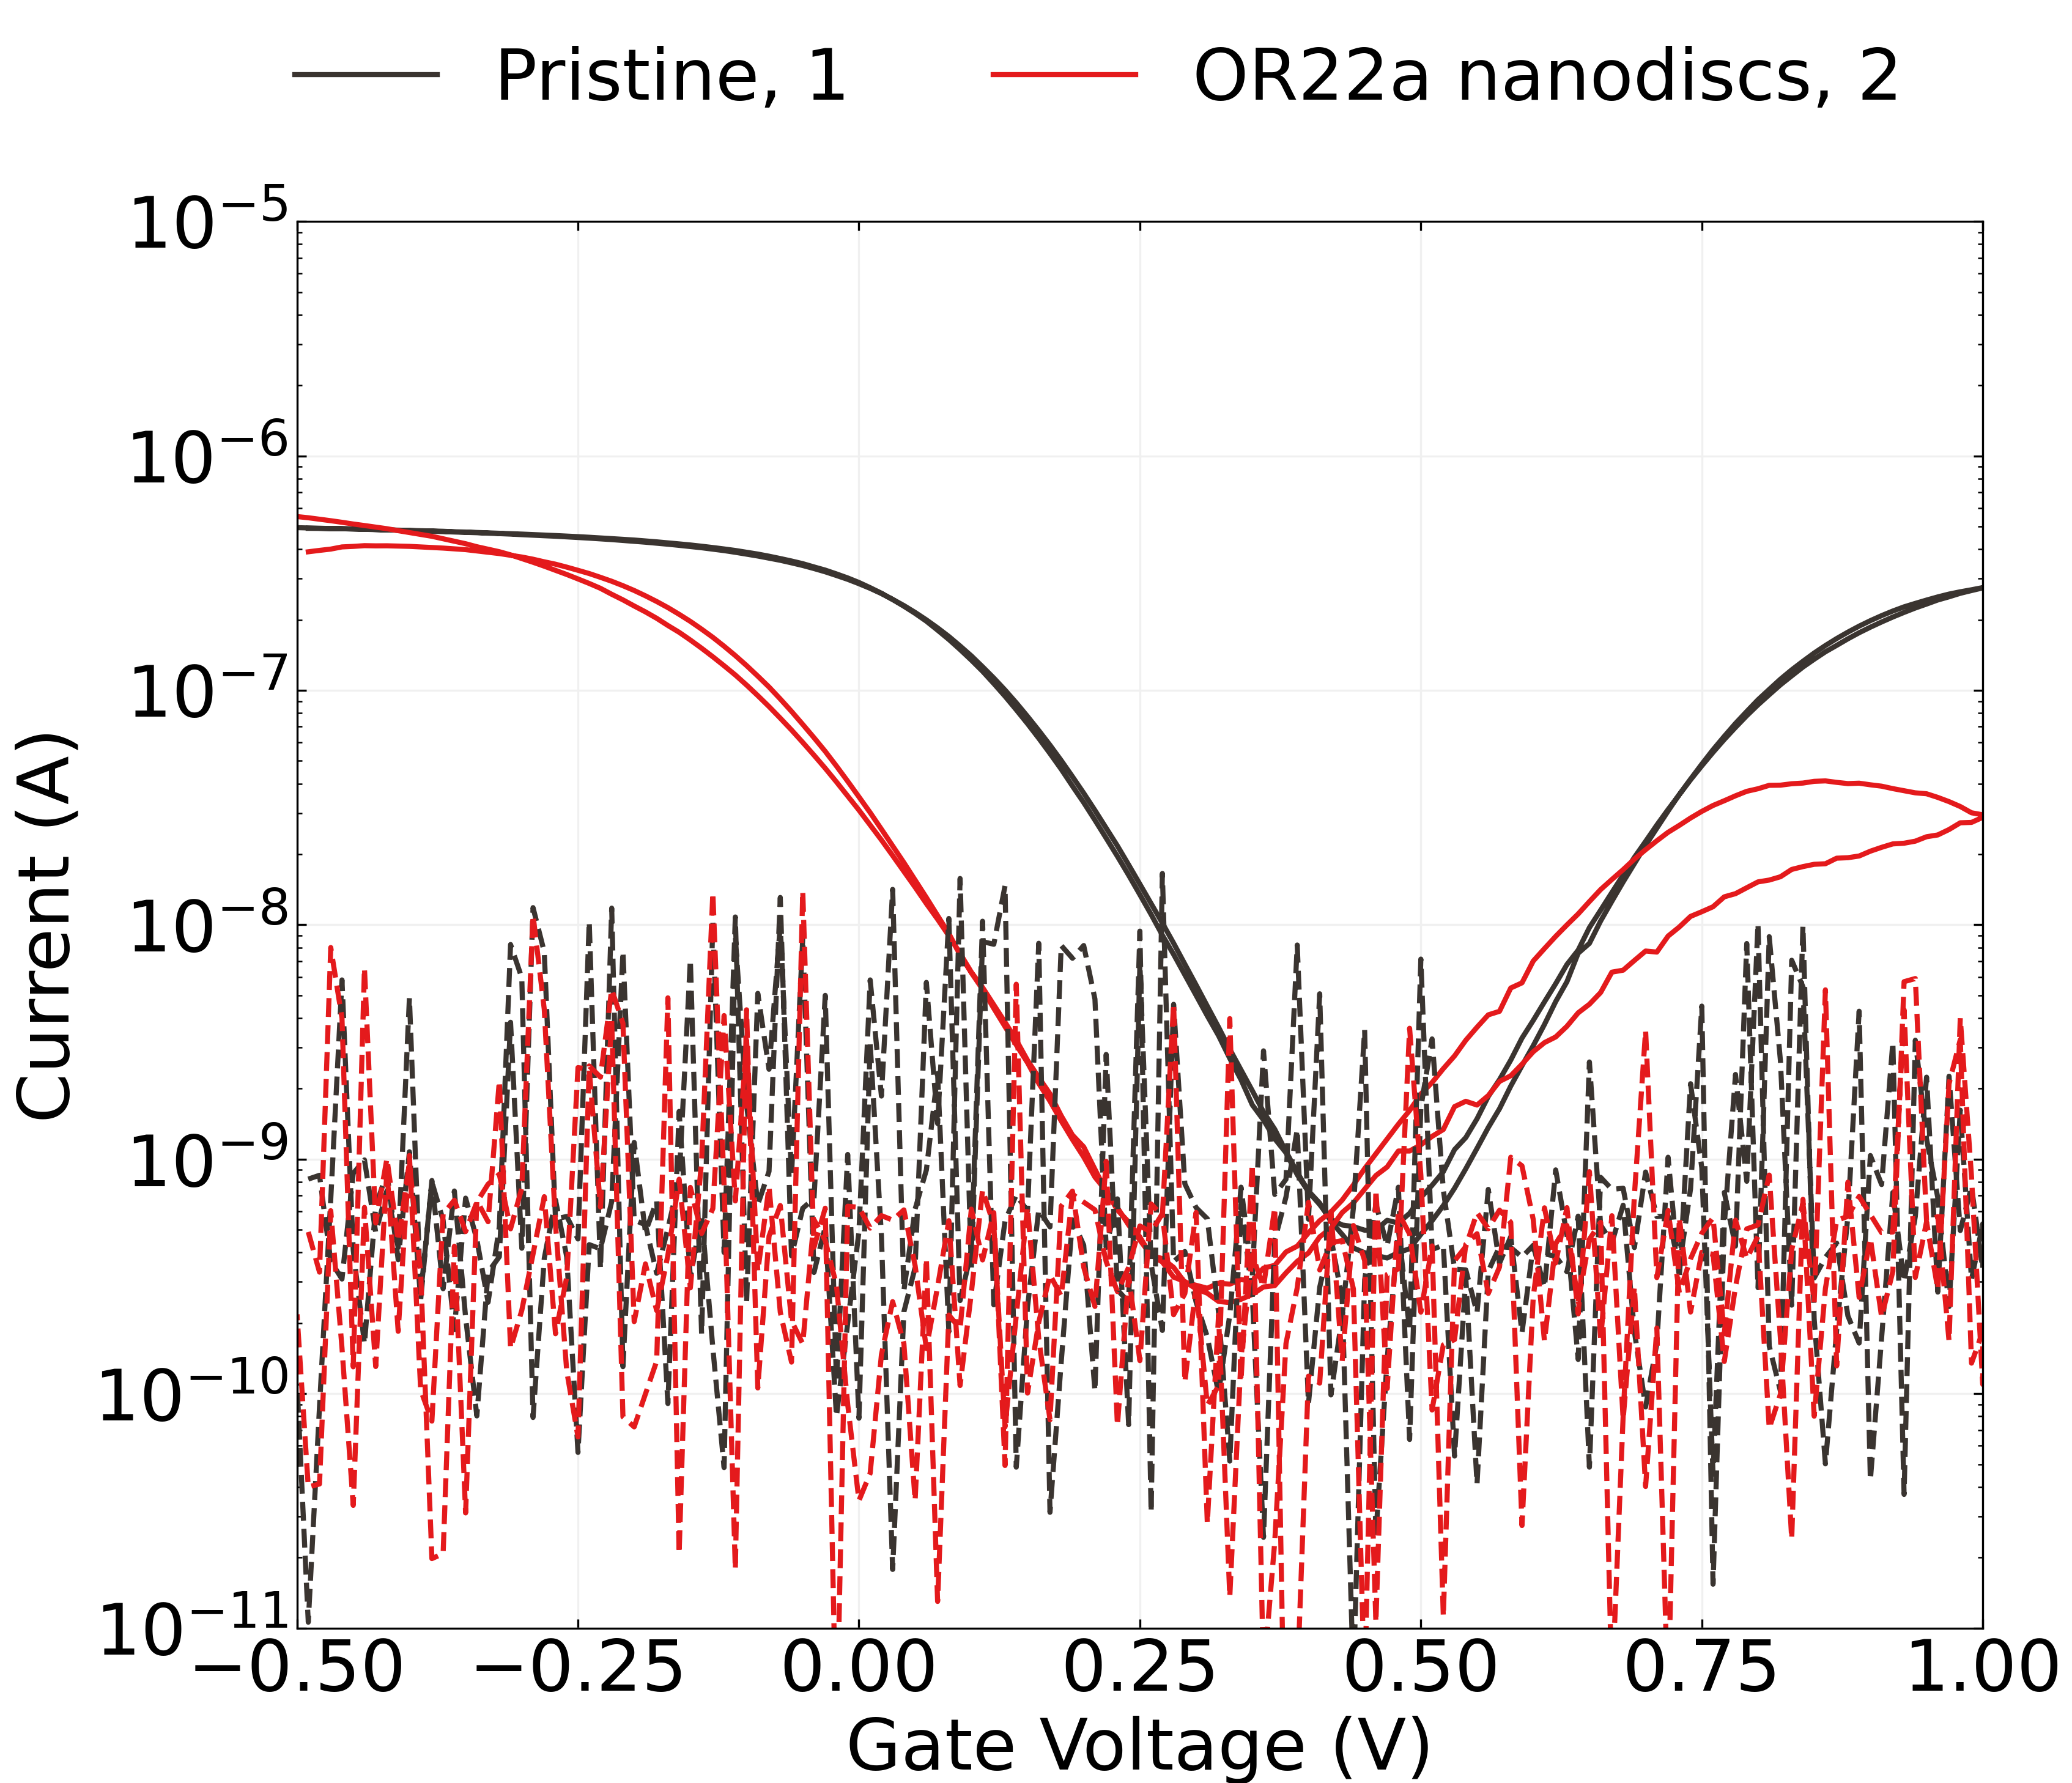
\includegraphics{figures/ch8/Q1C6_ch7_absolute_values_with_gate_current.png}

}

}

\end{minipage}%
%
\begin{minipage}[t]{0.01\linewidth}

{\centering 

~

}

\end{minipage}%
%
\begin{minipage}[t]{0.03\linewidth}

{\centering 

\raisebox{-\height}{

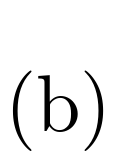
\includegraphics{figures/(b).png}

}

}

\end{minipage}%
%
\begin{minipage}[t]{0.01\linewidth}

{\centering 

~

}

\end{minipage}%
%
\begin{minipage}[t]{0.45\linewidth}

{\centering 

\raisebox{-\height}{

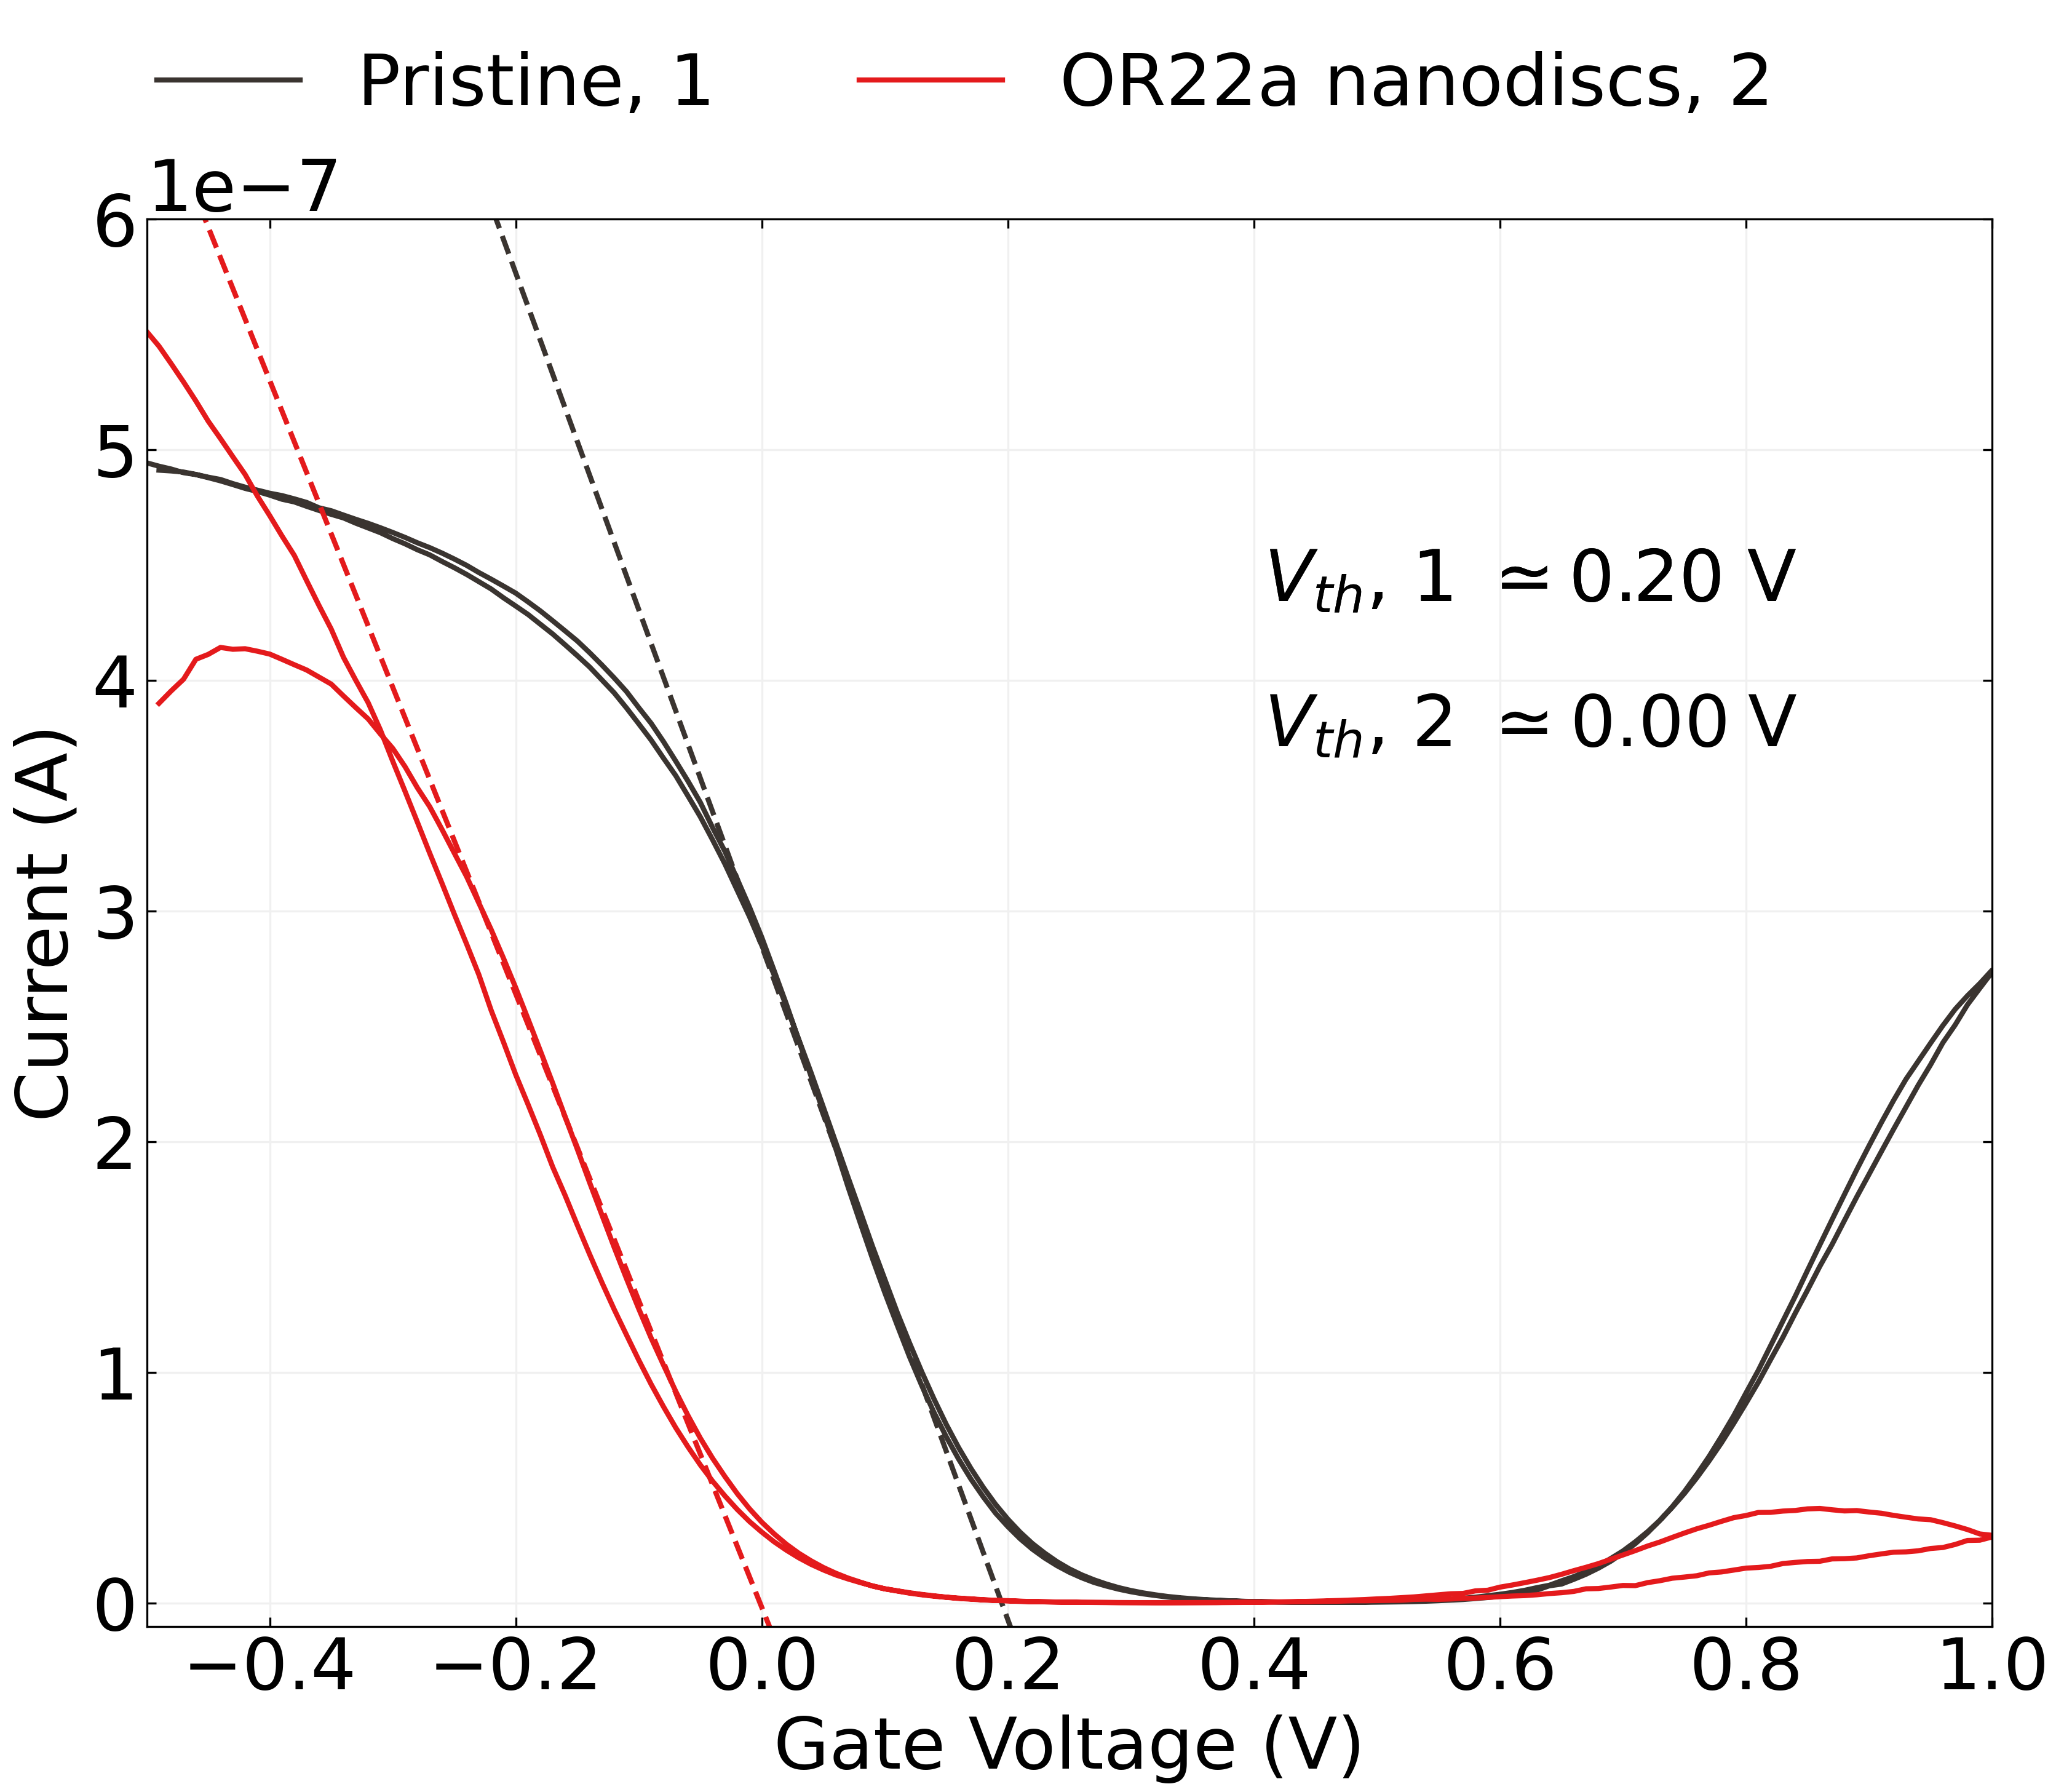
\includegraphics{figures/ch8/Q1C6_ch7_absolute_values_with_threshold_voltage_shift_without_gate_current.png}

}

}

\end{minipage}%
%
\begin{minipage}[t]{0.01\linewidth}

{\centering 

~

}

\end{minipage}%

\caption{\label{fig-OR22a-TX-comparison}Liquid-gated carbon nanotube
network device transfer characteristics before and after OR22a nanodisc
functionalisation. In (a), the characteristics are shown on a
logarithmic scale, where the gate current for each transfer curve is
shown with a dashed line. In (b), the characteristics are shown on a
linear scale alongside a dashed line tangent to the subthreshold slope
of the characteristic curve. The threshold voltage corresponding to the
intercept of this slope with the x-axis is shown for each transfer
characteristic curve.}

\end{figure}

Only minor changes were observed in the on-off ratio when comparing the
device channel before and after functionalisation. The on-off ratio for
the pristine channel was \(1120\pm220\), fairly typical for a transfer
curve from a steam-assisted surfactant-deposited CNT network device (see
\textbf{?@sec-cnt-devices}). The on-off ratio increased slightly to
\(1830\pm550\) after functionalisation. We expect to see an increase in
on-off ratio for a device successfully functionalised with OR22a, which
may result from an increase in negative charge causing modulation of
Schottky barriers between metallic and semiconducting carbon nanotubes
within the network \autocite{Murugathas2019b}. However, we also expect
increased hole conductance from the attachment of PBASE, even without
proteins being present
(\textbf{?@sec-PBASE-electrical-characterisation}). It is therefore
difficult to determine whether functionalisation has been successful
from the on-off ratio of transfer characteristics alone.

Functionalisation of the channel resulted in a negative shift in
threshold voltage of \(-0.20\pm0.03\) V. This is significantly in excess
of threshold voltage shifts measured for both methanol adsorption
(\(-0.15\pm0.02\) V) and after exposure to PBASE in methanol
(\(-0.06\pm0.04\) V), confirming that protein has attached to the carbon
nanotubes. However, both direct protein adsorption
\autocite{Bradley2004,Heller2008} and empty nanodisc attachment
\autocite{Murugathas2019b} should also lead to a significant negative
threshold voltage shift in the liquid-gated transfer characteristic
curve. In all three cases, the voltage shift is predominantly the result
of negative charge transfer from the adsorped proteins to the
semiconducting carbon nanotubes
\autocite{Bradley2004,Heller2008,Murugathas2019b}. It is likely that the
negative shift observed results from some combination of the three types
of attachment. It should be noted that while the size of the
functionalisation-induced threshold voltage shift can be used to
determine whether protein has attached to the nanodisc network, it
cannot be used to specifically determine whether odorant receptors have
attached to the network.

\begin{figure}

\begin{minipage}[t]{0.03\linewidth}

{\centering 

\raisebox{-\height}{


\includegraphics{figures/(a).png}

}

}

\end{minipage}%
%
\begin{minipage}[t]{0.01\linewidth}

{\centering 

~

}

\end{minipage}%
%
\begin{minipage}[t]{0.45\linewidth}

{\centering 

\raisebox{-\height}{

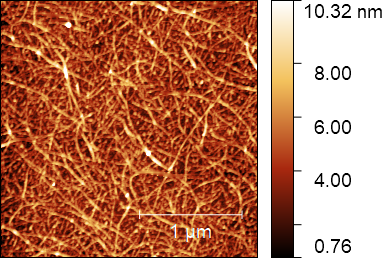
\includegraphics{figures/ch8/Pristine_DF2Q3D10_ 00141.png}

}

}

\end{minipage}%
%
\begin{minipage}[t]{0.01\linewidth}

{\centering 

~

}

\end{minipage}%
%
\begin{minipage}[t]{0.03\linewidth}

{\centering 

\raisebox{-\height}{

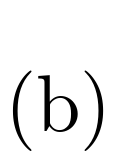
\includegraphics{figures/(b).png}

}

}

\end{minipage}%
%
\begin{minipage}[t]{0.01\linewidth}

{\centering 

~

}

\end{minipage}%
%
\begin{minipage}[t]{0.45\linewidth}

{\centering 

\raisebox{-\height}{

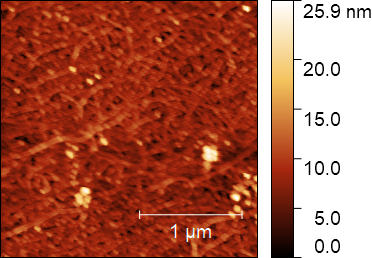
\includegraphics{figures/ch8/DF2Q1D6_postNDOR22a_ch7_1_00375.png}

}

}

\end{minipage}%
%
\begin{minipage}[t]{0.01\linewidth}

{\centering 

~

}

\end{minipage}%

\caption{\label{fig-working-OR22a-AFM}Atomic force microscope images of
the channel region of carbon nanotube network devices before and after
functionalisation. The channel network of a pristine device is shown in
(a), while (b) is of channel 7 from the sensing device functionalised in
this section.}

\end{figure}

Atomic force microscope images of the device channels both before
functionalisation and after sensing with the functionalised device to
confirm the presence of nanodiscs. As far as the author knows, these are
the first atomic force microscope images taken of iOR nanodiscs found on
a sensing channel rather than on a separate carbon nanotube film; the
wider 20 µm encapsulation mask discussed in \textbf{?@sec-encapsulation}
made this possible. These images are shown in
Figure~\ref{fig-working-OR22a-AFM}. Aggregations of nanodiscs are
visible in Figure~\ref{fig-working-OR22a-AFM} (c)\(-\)(d). These
nanodisc clusters are especially sizable in the lower half of
Figure~\ref{fig-working-OR22a-AFM} (c), where the two largest clusters
are \(200\pm10\) nm across at their widest point. However, these
features are still much smaller than most of the agglomerated nanodisc
features seen by Murugathas \emph{et al.} \autocite{Murugathas2019b}.
Furthermore, the nanodisc features closely follow the carbon nanotube
bundles across the densely bundled morphology used by Murugathas
\emph{et al.} \autocite{Murugathas2019b}. On the dense network
morphology used here, the position of nanodisc clusters relative to the
carbon nanotubes is less distinct. To confirm whether nanodiscs have
preferentially attached to the carbon nanotubes, a more quantitative
approach is needed.

\begin{figure}

\begin{minipage}[t]{0.03\linewidth}

{\centering 

\raisebox{-\height}{


\includegraphics{figures/(a).png}

}

}

\end{minipage}%
%
\begin{minipage}[t]{0.01\linewidth}

{\centering 

~

}

\end{minipage}%
%
\begin{minipage}[t]{0.45\linewidth}

{\centering 

\raisebox{-\height}{

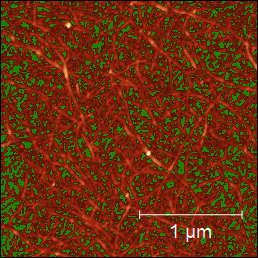
\includegraphics{figures/ch8/Pristine_DF2Q3D10_ 00141_mask.png}

}

}

\end{minipage}%
%
\begin{minipage}[t]{0.01\linewidth}

{\centering 

~

}

\end{minipage}%
%
\begin{minipage}[t]{0.03\linewidth}

{\centering 

\raisebox{-\height}{

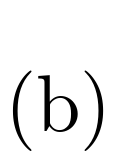
\includegraphics{figures/(b).png}

}

}

\end{minipage}%
%
\begin{minipage}[t]{0.01\linewidth}

{\centering 

~

}

\end{minipage}%
%
\begin{minipage}[t]{0.45\linewidth}

{\centering 

\raisebox{-\height}{

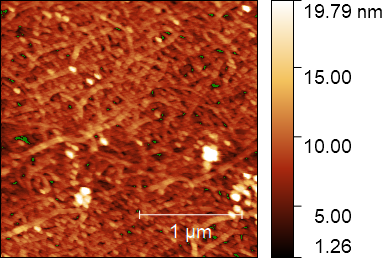
\includegraphics{figures/ch8/DF2Q1D6_postNDOR22a_ch7_1_00375_mask.png}

}

}

\end{minipage}%
%
\begin{minipage}[t]{0.01\linewidth}

{\centering 

~

}

\end{minipage}%

\caption{\label{fig-working-OR22a-masks}Atomic force microscope images
with the substrate background highlighted with a green mask. Here, (a)
shows a device channel after functionalisation with PBASE and methanol,
while (b) shows channel 7 from the sensing device functionalised with
OR22a nanodiscs in this section.}

\end{figure}

\begin{figure}

\begin{minipage}[t]{0.03\linewidth}

{\centering 

\raisebox{-\height}{


\includegraphics{figures/(a).png}

}

}

\end{minipage}%
%
\begin{minipage}[t]{0.01\linewidth}

{\centering 

~

}

\end{minipage}%
%
\begin{minipage}[t]{0.45\linewidth}

{\centering 

\raisebox{-\height}{

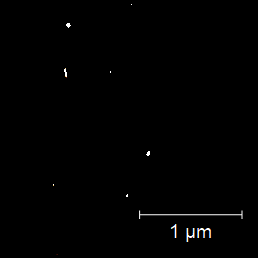
\includegraphics{figures/ch8/Pristine_DF2Q3D10_ 00141_11.2nm_crosssection.png}

}

}

\end{minipage}%
%
\begin{minipage}[t]{0.01\linewidth}

{\centering 

~

}

\end{minipage}%
%
\begin{minipage}[t]{0.03\linewidth}

{\centering 

\raisebox{-\height}{

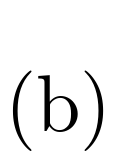
\includegraphics{figures/(b).png}

}

}

\end{minipage}%
%
\begin{minipage}[t]{0.01\linewidth}

{\centering 

~

}

\end{minipage}%
%
\begin{minipage}[t]{0.45\linewidth}

{\centering 

\raisebox{-\height}{

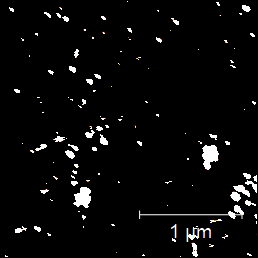
\includegraphics{figures/ch8/DF2Q1D6_postNDOR22a_ch7_1_00375_12nm_crosssection.png}

}

}

\end{minipage}%
%
\begin{minipage}[t]{0.01\linewidth}

{\centering 

~

}

\end{minipage}%

\caption{\label{fig-crosssection}Binary representations of the atomic
force microscope images of (a) the pristine device, with a threshold
height of 11.2 nm, and (b) the functionalised device, with a threshold
height of 12 nm. Both thresholds are 8.7 nm above the substrate
background of their respective images.}

\end{figure}

The average height of the substrate was found for both pristine and
functionalised atomic force microscope images using the masking tool in
Gwyddion. The masks for each image are shown in
Figure~\ref{fig-working-OR22a-masks}. Average substrate heights of
\(2.5\pm0.2\) nm and \(3.3\pm0.4\) nm were found for the pristine and
functionalised networks respectively, both within one standard deviation
of the substrate height of the steam-assisted surfactant-deposited film
analysed in \textbf{?@sec-pristine-AFM}. In Gwyddion, both networks were
simplified to a binary representation, where features above a certain
threshold were shown as white and features below shown as black, as
shown in Figure~\ref{fig-crosssection}. This representation has the
appearance of a cross-section through the network at the threshold
height. The threshold was chosen as the minimum height where carbon
nanotube spindles were no longer apparent in the functionalised image,
8.7 nm above the substrate. Figure~\ref{fig-crosssection} (a) shows only
a few, sparsely distributed features, the majority of which are below 50
nm. These features may correspond to surfactant or other surface
contamination (\textbf{?@sec-pristine-morphology}). In
Figure~\ref{fig-crosssection} (b), many features are over 50 nm across,
and often form clusters which sometimes follow curved lines across the
network; these patterns give a strong indication that nanodiscs are
attaching to the carbon nanotubes.

As the maximum height of the functionalised AFM is 25.9 nm and only
nanodisc features are present at 12.0 nm, there must be nanodisc
agglomerates present at least 13.9 nm tall. The estimated height range
for nanodiscs is \(\sim\) 10 \(-\) 20 nm
\autocite{Nath2007,Bayburt2010,Murugathas2020}. Assuming a average
carbon nanotube height of 1.45 nm, with a average substrate height of
3.3 nm, the nanodisc agglomerations could be up to \(\sim\) 21 nm tall.
Note that height measurements of biological samples taken via AFM have
been shown to underestimate actual feature height by over 50\%
\autocite{Vobornik2023}. Even so, the breadths of the nanodisc features
are significantly greater than their heights. While the cross-sections
of the largest features are up to 20 nanodiscs across, they are a few
nanodiscs high at most; certainly less than five. It appears that,
rather than clustering together in solution and attaching as an
aggregate, the nanodiscs are individually attaching to preferred
locations on the network. These locations may be at junctions between
two large carbon nanotubes, which have a relatively large surface area
available for binding, or at locations particularly clean of
contamination. AFM images showing iOR-nanodisc functionalised carbon
nanotube networks with significant vertical clustering have been
reported, but these images were not of channels used for sensing
\autocite{Murugathas2019b}.

\hypertarget{sec-EtHex-aqueous-sensing}{%
\subsection{Aqueous Sensing of Ethyl
Hexanoate}\label{sec-EtHex-aqueous-sensing}}

The procedure used for biosensor detection of ethyl hexanoate in liquid
was the same as the procedure outlined in \textbf{?@sec-dummy-sensing},
except 0.5\% DMSO was present in the buffer solution (to improve ethyl
hexanoate solubility) and dilutions of ethyl hexanoate in the same 0.5\%
DMSO 1XPBS buffer solution were added during the sensing series. The
0.5\% DMSO 1XPBS was prepared by adding 5 µL of DMSO to 995 µL 1XPBS
before device characterisation. The dilutions of ethyl hexanoate were
prepared with the same 1XPBS at the same time, where 5 µL of 200 fM, 200
pM, 200 nM and 200 µM ethyl hexanoate in DMSO were placed into four
individual vials containing 995 µL 1XPBS each, giving 1mL vials of 1 fM,
1 pM, 1 nM and 1 µM ethyl hexanoate in 0.5\% DMSO 1XPBS. The ethyl
hexanoate in DMSO dilutions were prepared beforehand as a 1:10 dilution
series in DMSO using 200 mM stock solution, where dilutions ranged from
20 mM to 200 fM. Sampling measurements were taken using the B1500A
semiconductor device analyser, with the transfer measurement in
Figure~\ref{fig-OR22a-TX-comparison} (b) taken directly before sensing.
The full control series plus sensing sequence is shown in
Figure~\ref{fig-EtHex-aqueous-sensing}. Gate current remained negligible
across the entire sensing procedure.

\begin{figure}

{\centering 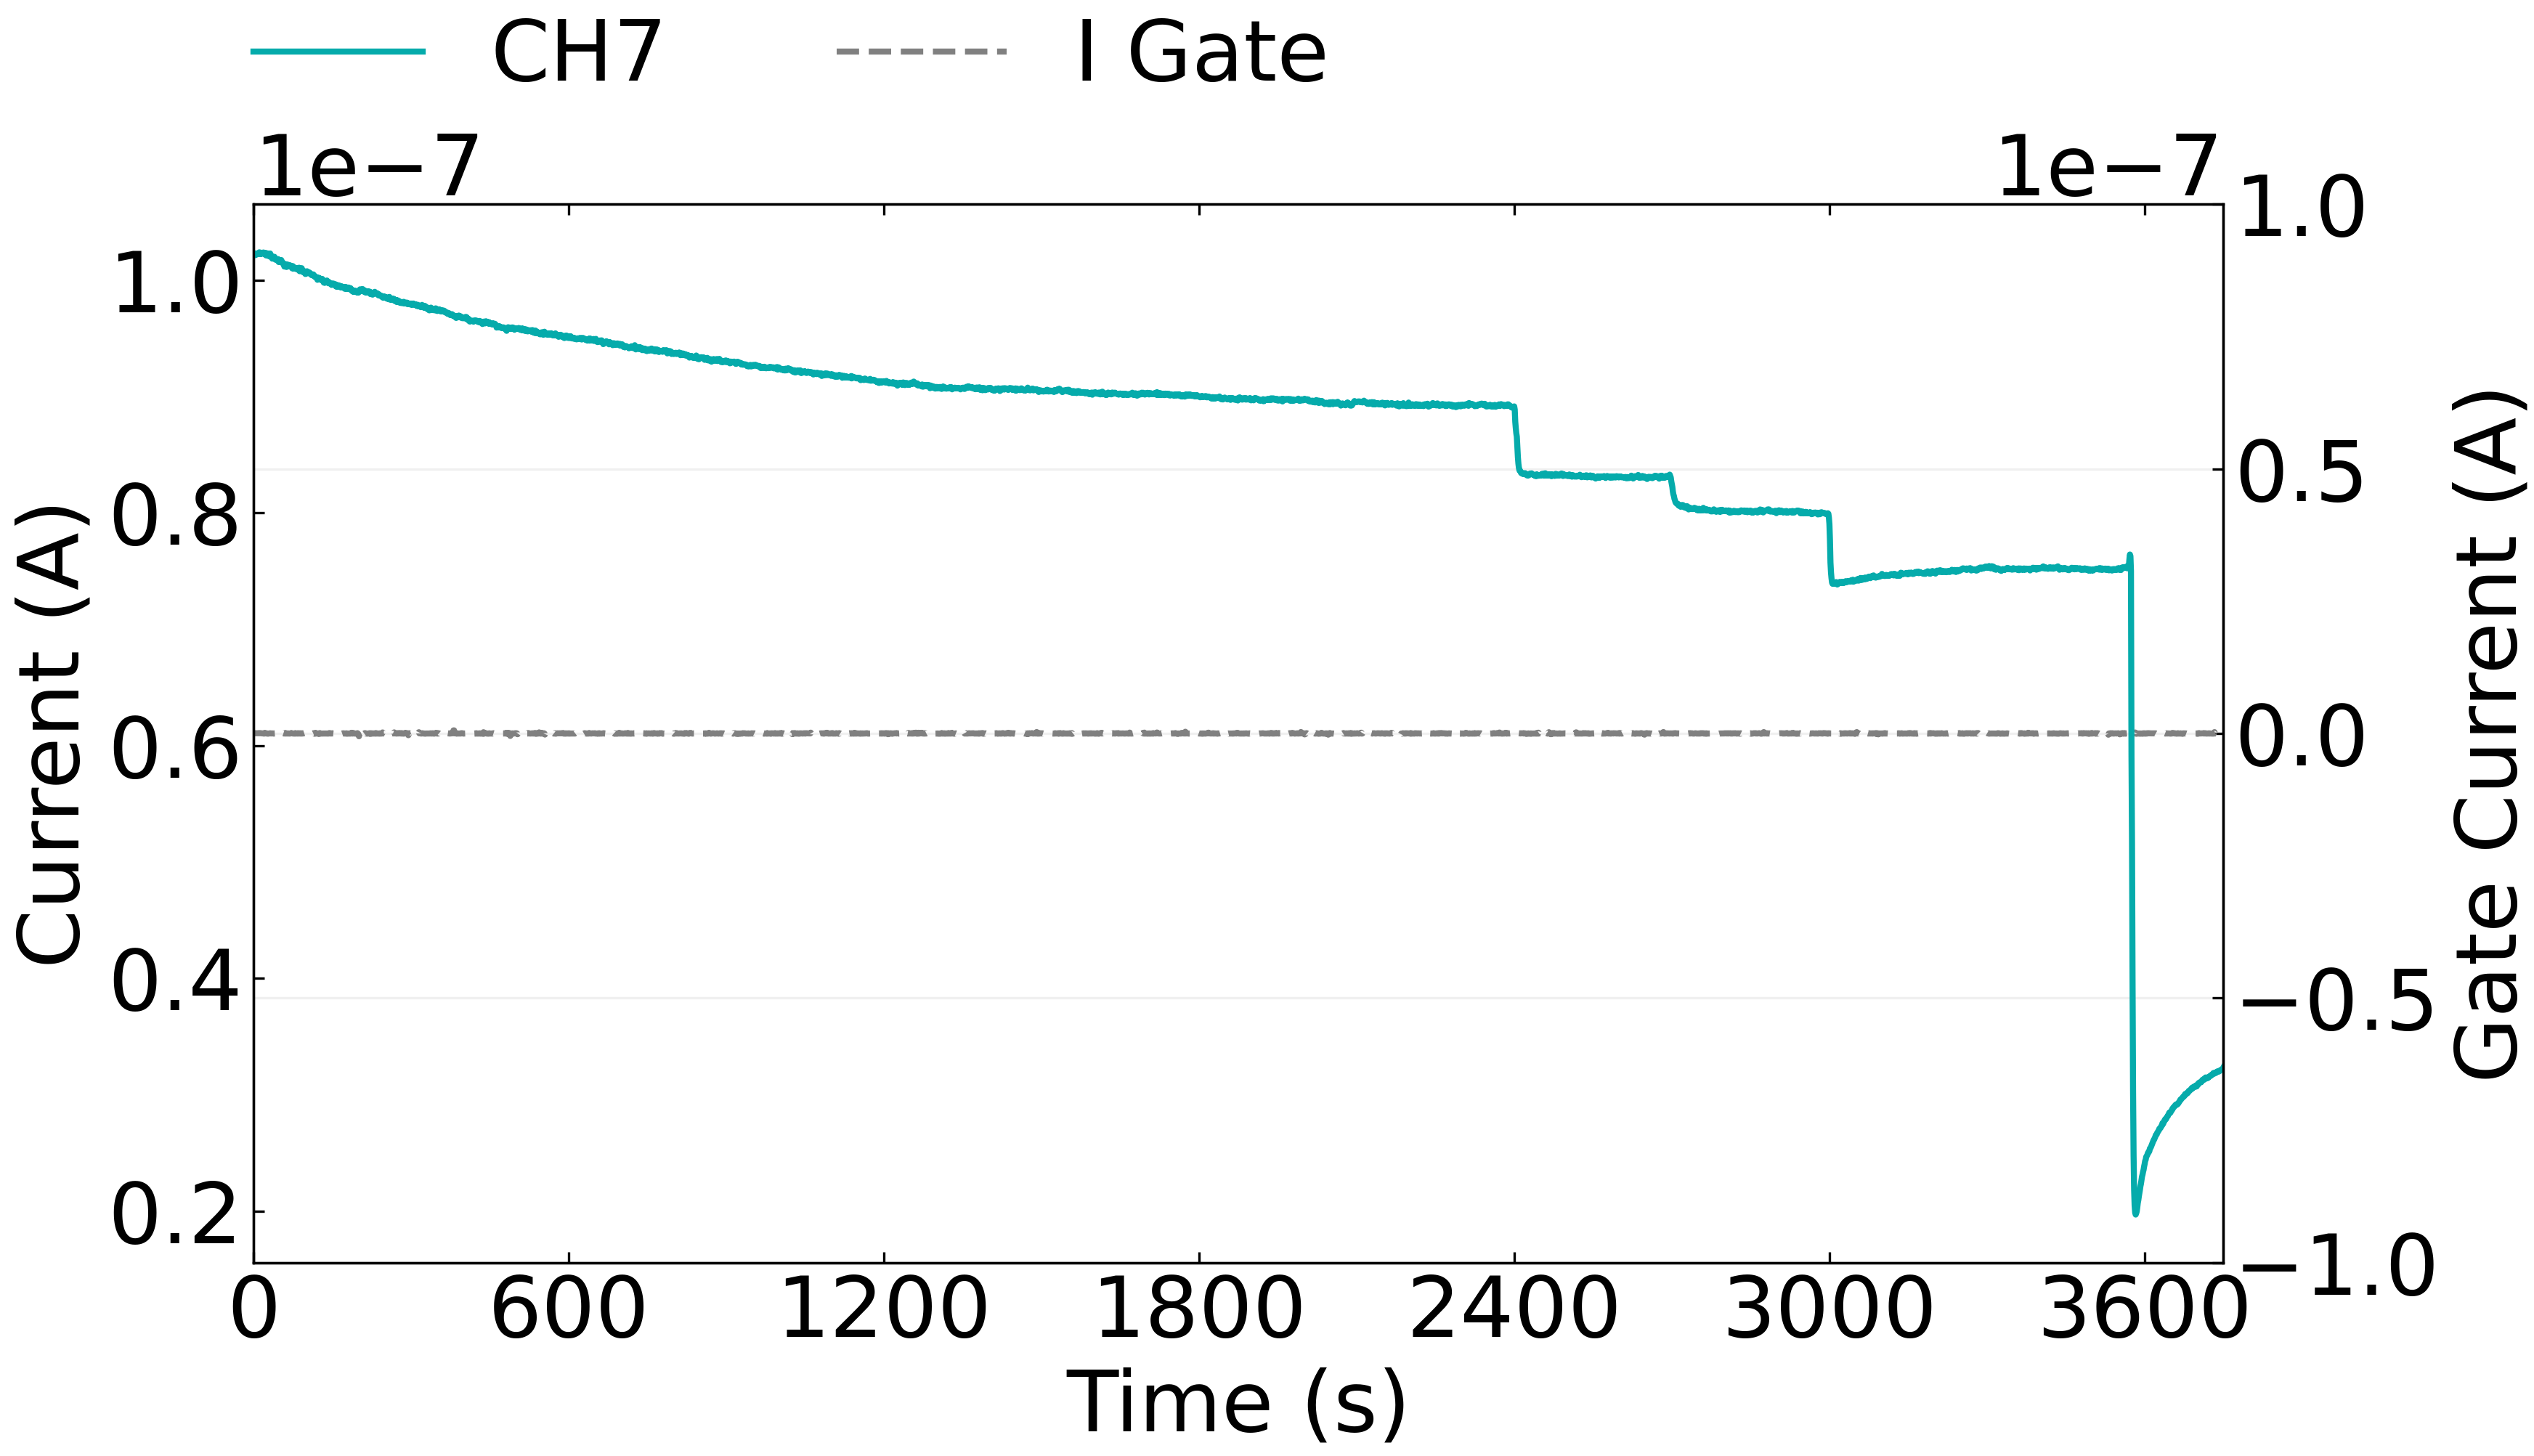
\includegraphics[width=0.7\textwidth,height=\textheight]{figures/ch8/Q1C6.png}

}

\caption{\label{fig-EtHex-aqueous-sensing}The control series (before
1800 s) and ethyl hexanoate sensing series (after 1800 s) of the
OR22a-functionalised device channel. No responses to 0.5\% DMSO 1XPBS
were seen during the control series, while significant responses to
additions of ethyl hexanoate diluted in 0.5\% DMSO 1XPBS were seen at
2400 s, 2700 s, 3000 s and 3600 s.}

\end{figure}

The control series for the sensing series is shown in
Figure~\ref{fig-OR22a-control-series} (a). No clear stepwise response is
seen to buffer additions or subtractions. The functionalised device
shows similar baseline drift behaviour to that of a pristine device,
with a period of short-term decay quickly yielding to a more long-lived
decay behaviour. A linear fit \(I = c_1t + c_2\) to the region
\(1200-1800\) had a gradient of \(c_1 = -1.76\pm0.02\) pA/s. This
gradient is smaller than the range of values found for the linear fit
approximating the longer-term drift of a pristine device
(\textbf{?@sec-baseline-drift}), but of the same order of magnitude. The
linear fit was then subtracted from the control series and an
exponential fit \(I = I_0\exp(-t/\tau)\) was performed on the remaining
dataset, as shown in Figure~\ref{fig-OR22a-control-series} (b). A value
of \(590 \pm 3\) s was found for the exponential time constant, similar
to those found for the channels of the pristine device. This confirms
that the 1800 s control series is sufficient to avoid the presence of
short-term decay during sensing.

\begin{figure}

\begin{minipage}[t]{0.11\linewidth}

{\centering 

~

}

\end{minipage}%
%
\begin{minipage}[t]{0.03\linewidth}

{\centering 

\raisebox{-\height}{


\includegraphics{figures/(a).png}

}

}

\end{minipage}%
%
\begin{minipage}[t]{0.01\linewidth}

{\centering 

~

}

\end{minipage}%
%
\begin{minipage}[t]{0.70\linewidth}

{\centering 

\raisebox{-\height}{

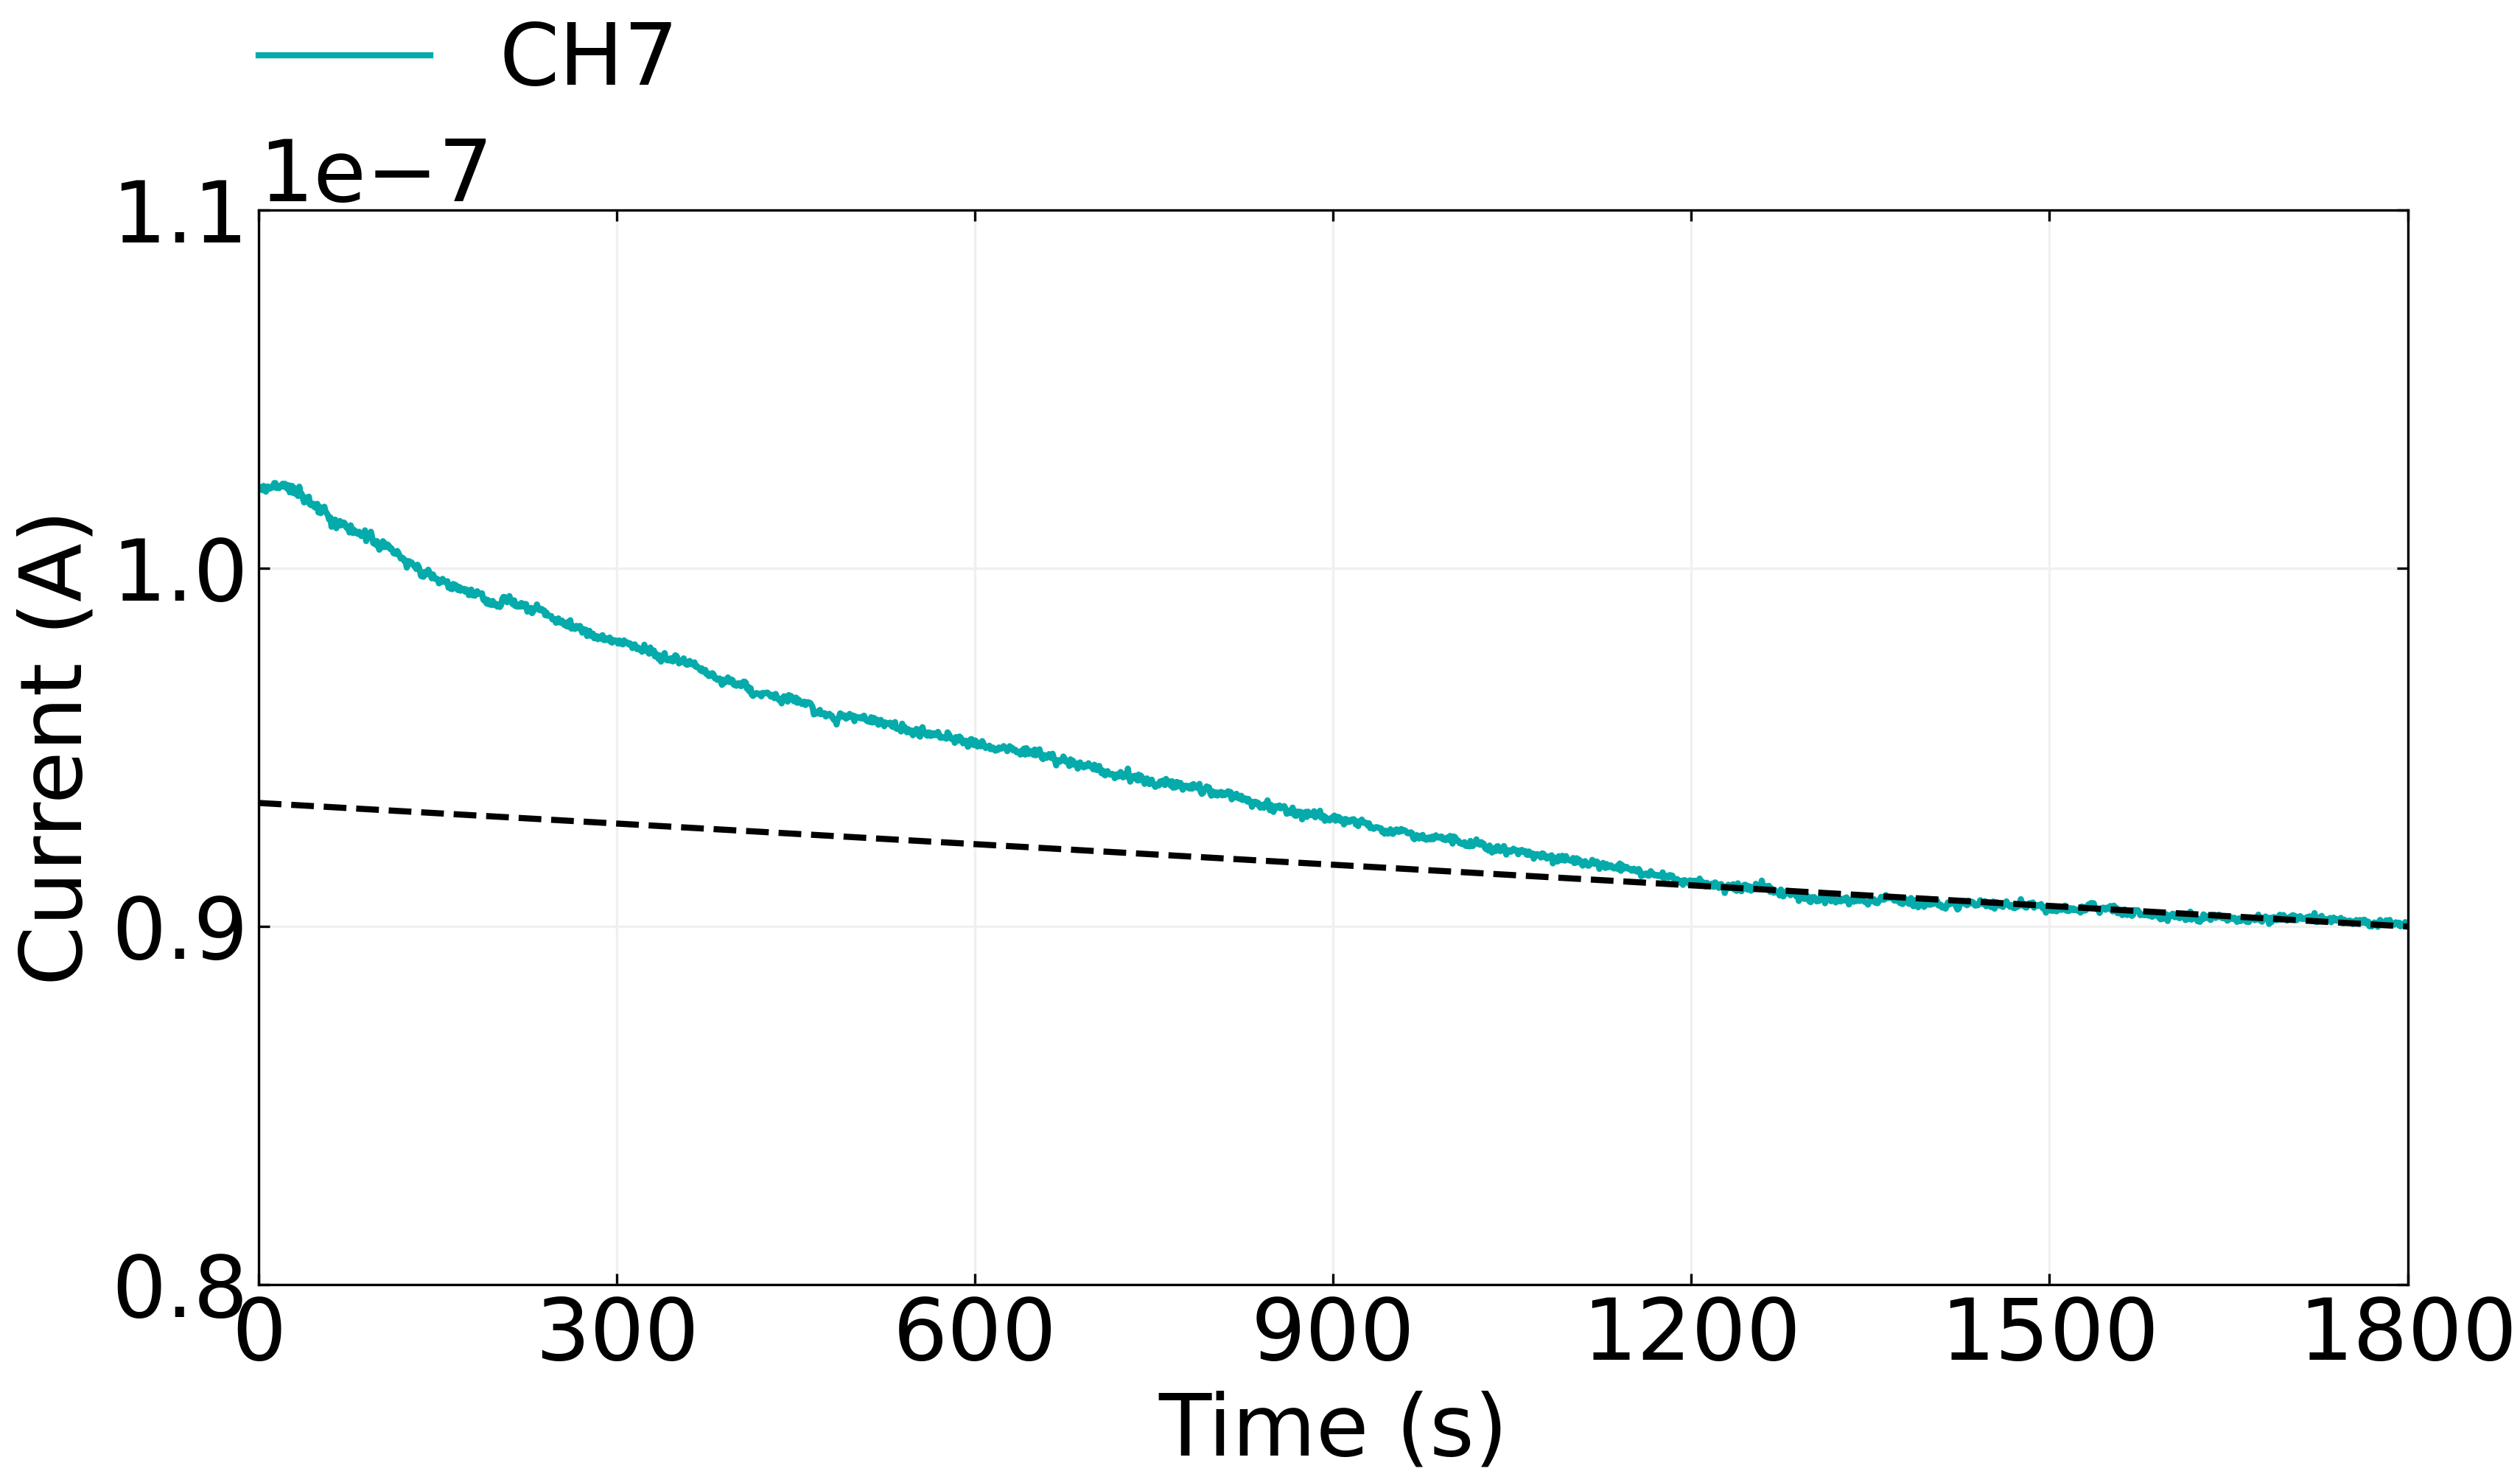
\includegraphics{figures/ch8/Q1C6_with_fitted_curves.png}

}

}

\end{minipage}%
%
\begin{minipage}[t]{0.15\linewidth}

{\centering 

~

}

\end{minipage}%
\newline
\begin{minipage}[t]{0.11\linewidth}

{\centering 

~

}

\end{minipage}%
%
\begin{minipage}[t]{0.03\linewidth}

{\centering 

\raisebox{-\height}{

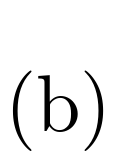
\includegraphics{figures/(b).png}

}

}

\end{minipage}%
%
\begin{minipage}[t]{0.01\linewidth}

{\centering 

~

}

\end{minipage}%
%
\begin{minipage}[t]{0.70\linewidth}

{\centering 

\raisebox{-\height}{

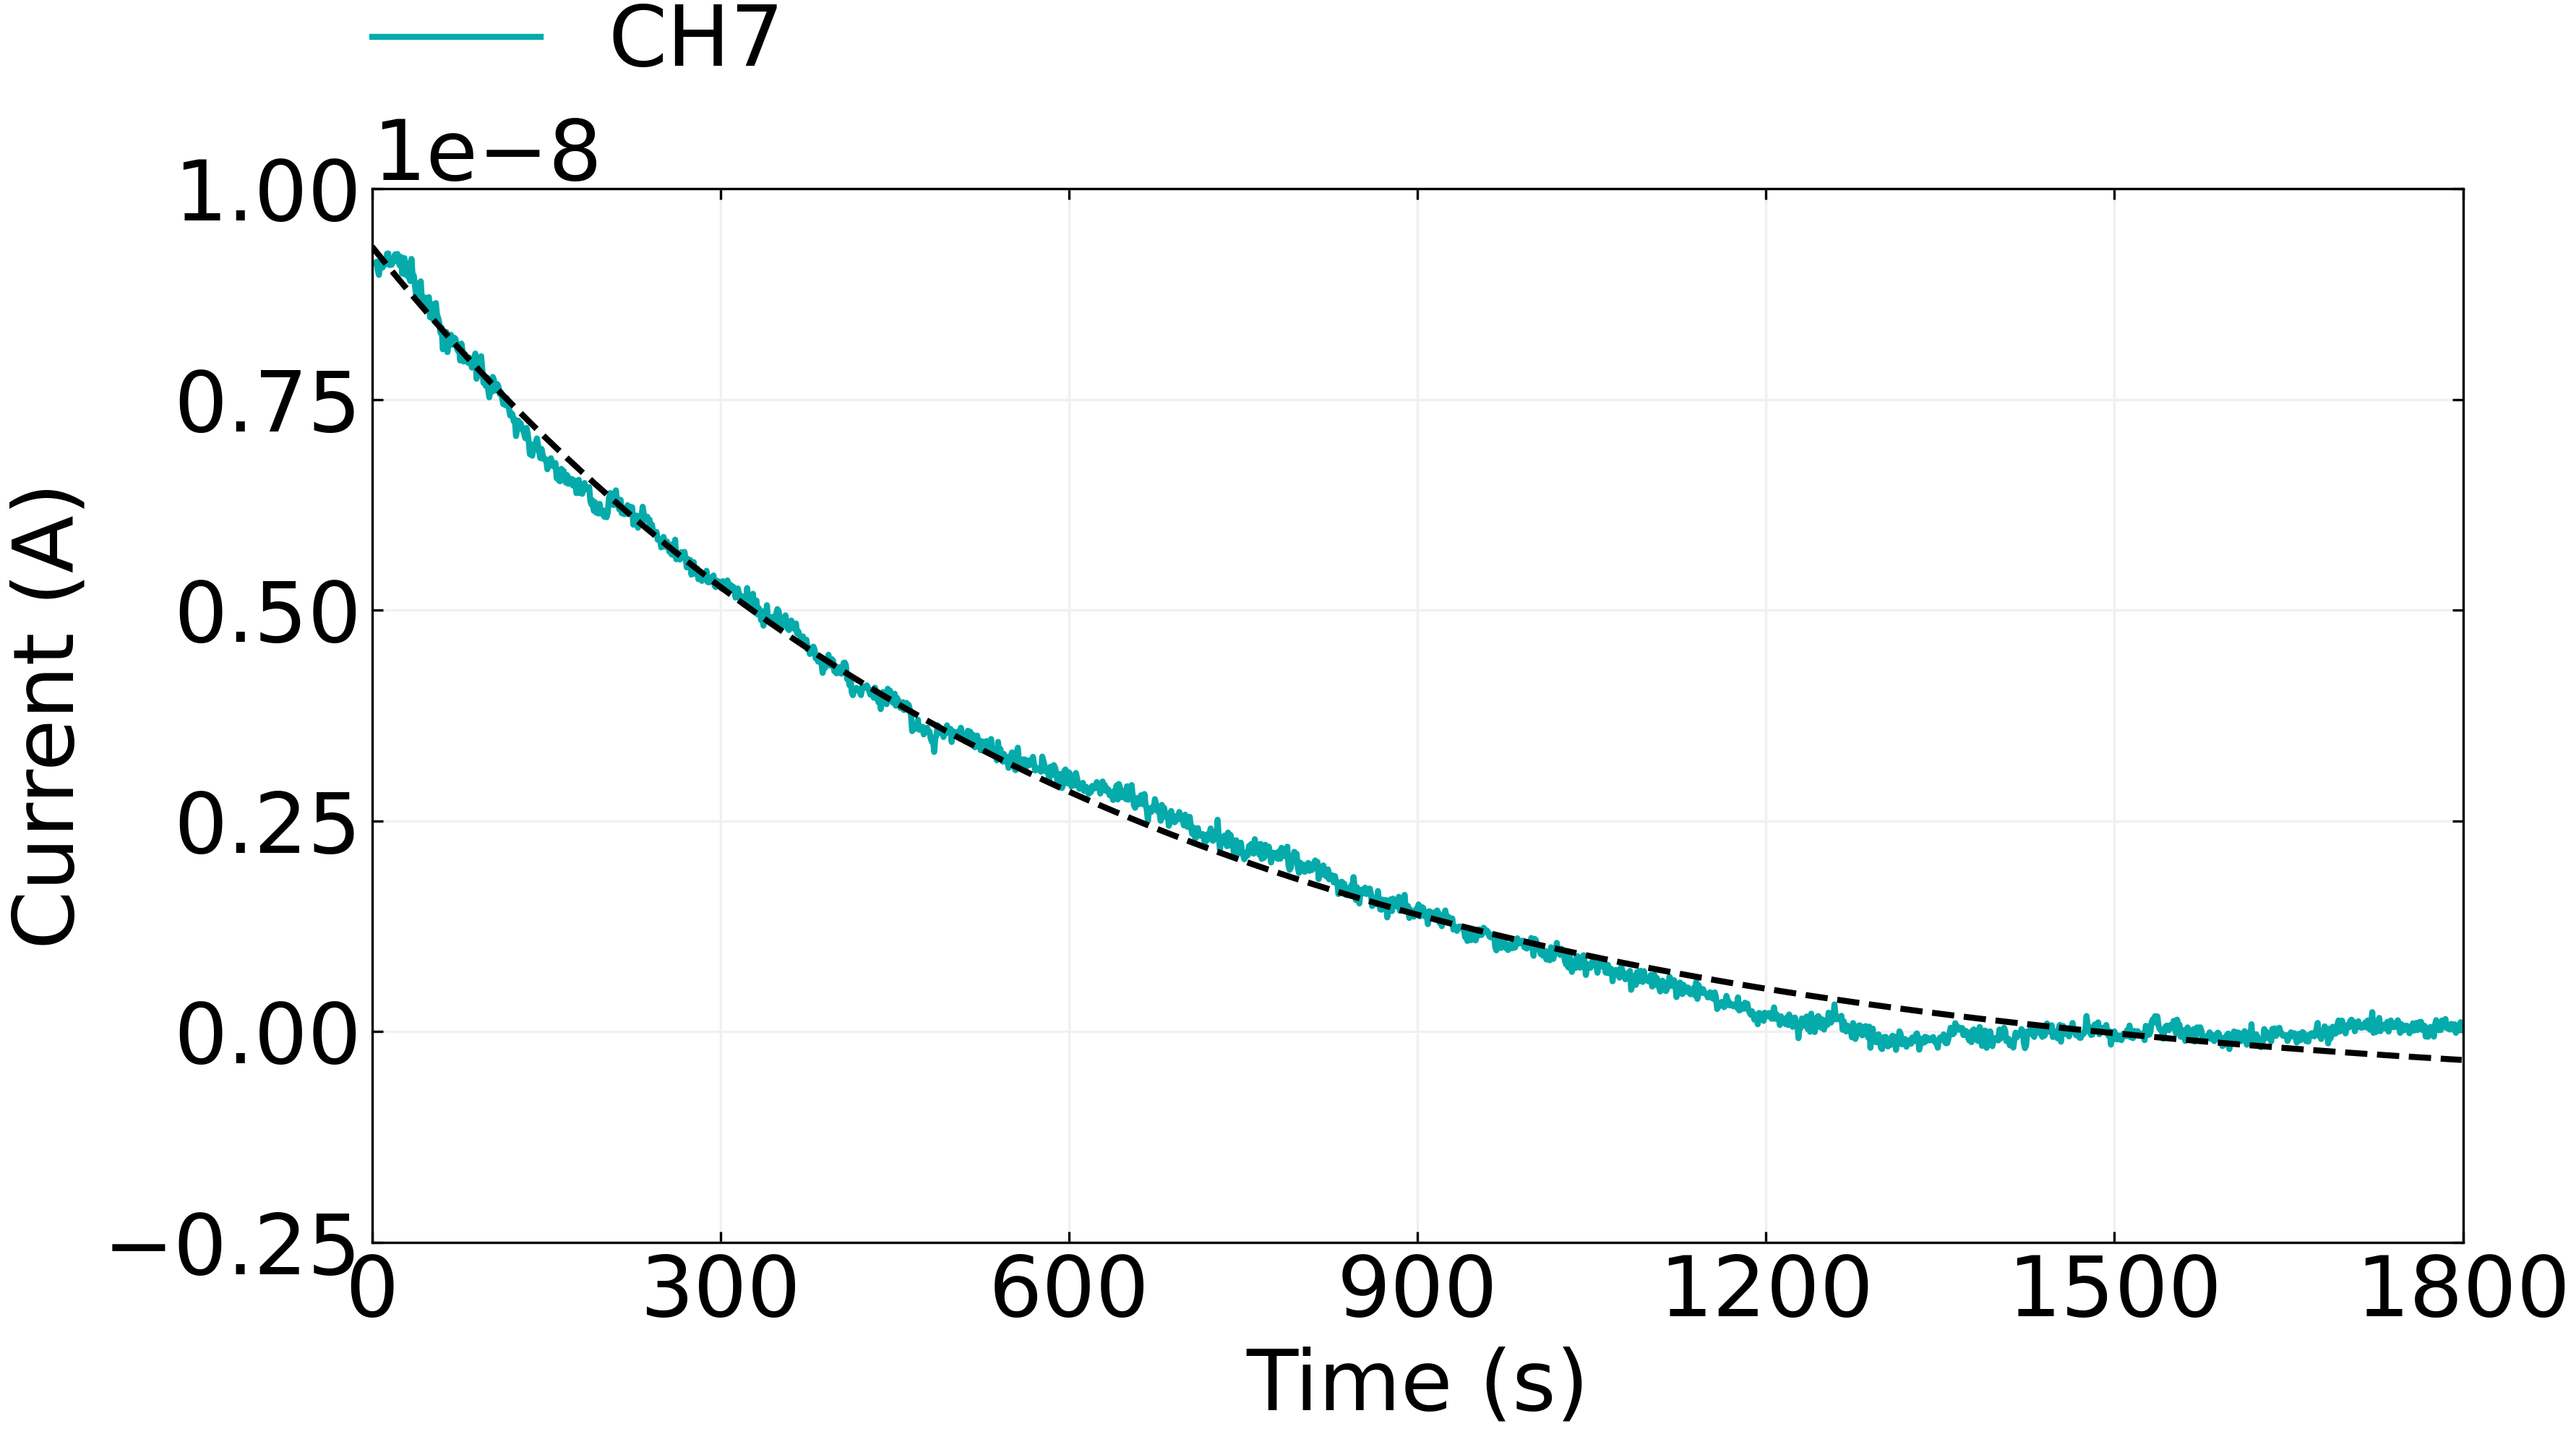
\includegraphics{figures/ch8/Q1C6_with_fitted_curves_exp.png}

}

}

\end{minipage}%
%
\begin{minipage}[t]{0.15\linewidth}

{\centering 

~

}

\end{minipage}%

\caption{\label{fig-OR22a-control-series}The control series for the
OR22a-functionalised device is shown in (a), alongside an extrapolated
linear fit to the control series from 1200 s onwards. The control series
with the linear approximation subtracted fitted to an exponential curve
is shown in (b).}

\end{figure}

It appears that the exponential fit overestimates current measurements
between 1100 s and 1500 s and underestimates between 1500 s and 1800 s.
This deviation from the fit may result from the linear approximation
used to represent long-term baseline drift being weaker for this channel
than for those discussed previously in \textbf{?@sec-dummy-sensing} and
\textbf{?@sec-pristine-EtHex}. This could result from the exponential
terms for long-term baseline drift having relatively short time
constants, so \(t\ll\tau_i\) no longer holds and higher order terms in
the linear approximation are no longer negligible. This observation may
indicate a relationship exists between device functionalisation and the
long-lived device decay behaviour. However, it may simply result from
the natural variation between randomly-deposited device channels.
Further work may be required to confirm the existence of such a
relationship, though this work is outside the scope of this thesis.

\begin{figure}

\begin{minipage}[t]{0.11\linewidth}

{\centering 

~

}

\end{minipage}%
%
\begin{minipage}[t]{0.03\linewidth}

{\centering 

\raisebox{-\height}{


\includegraphics{figures/(a).png}

}

}

\end{minipage}%
%
\begin{minipage}[t]{0.01\linewidth}

{\centering 

~

}

\end{minipage}%
%
\begin{minipage}[t]{0.70\linewidth}

{\centering 

\raisebox{-\height}{

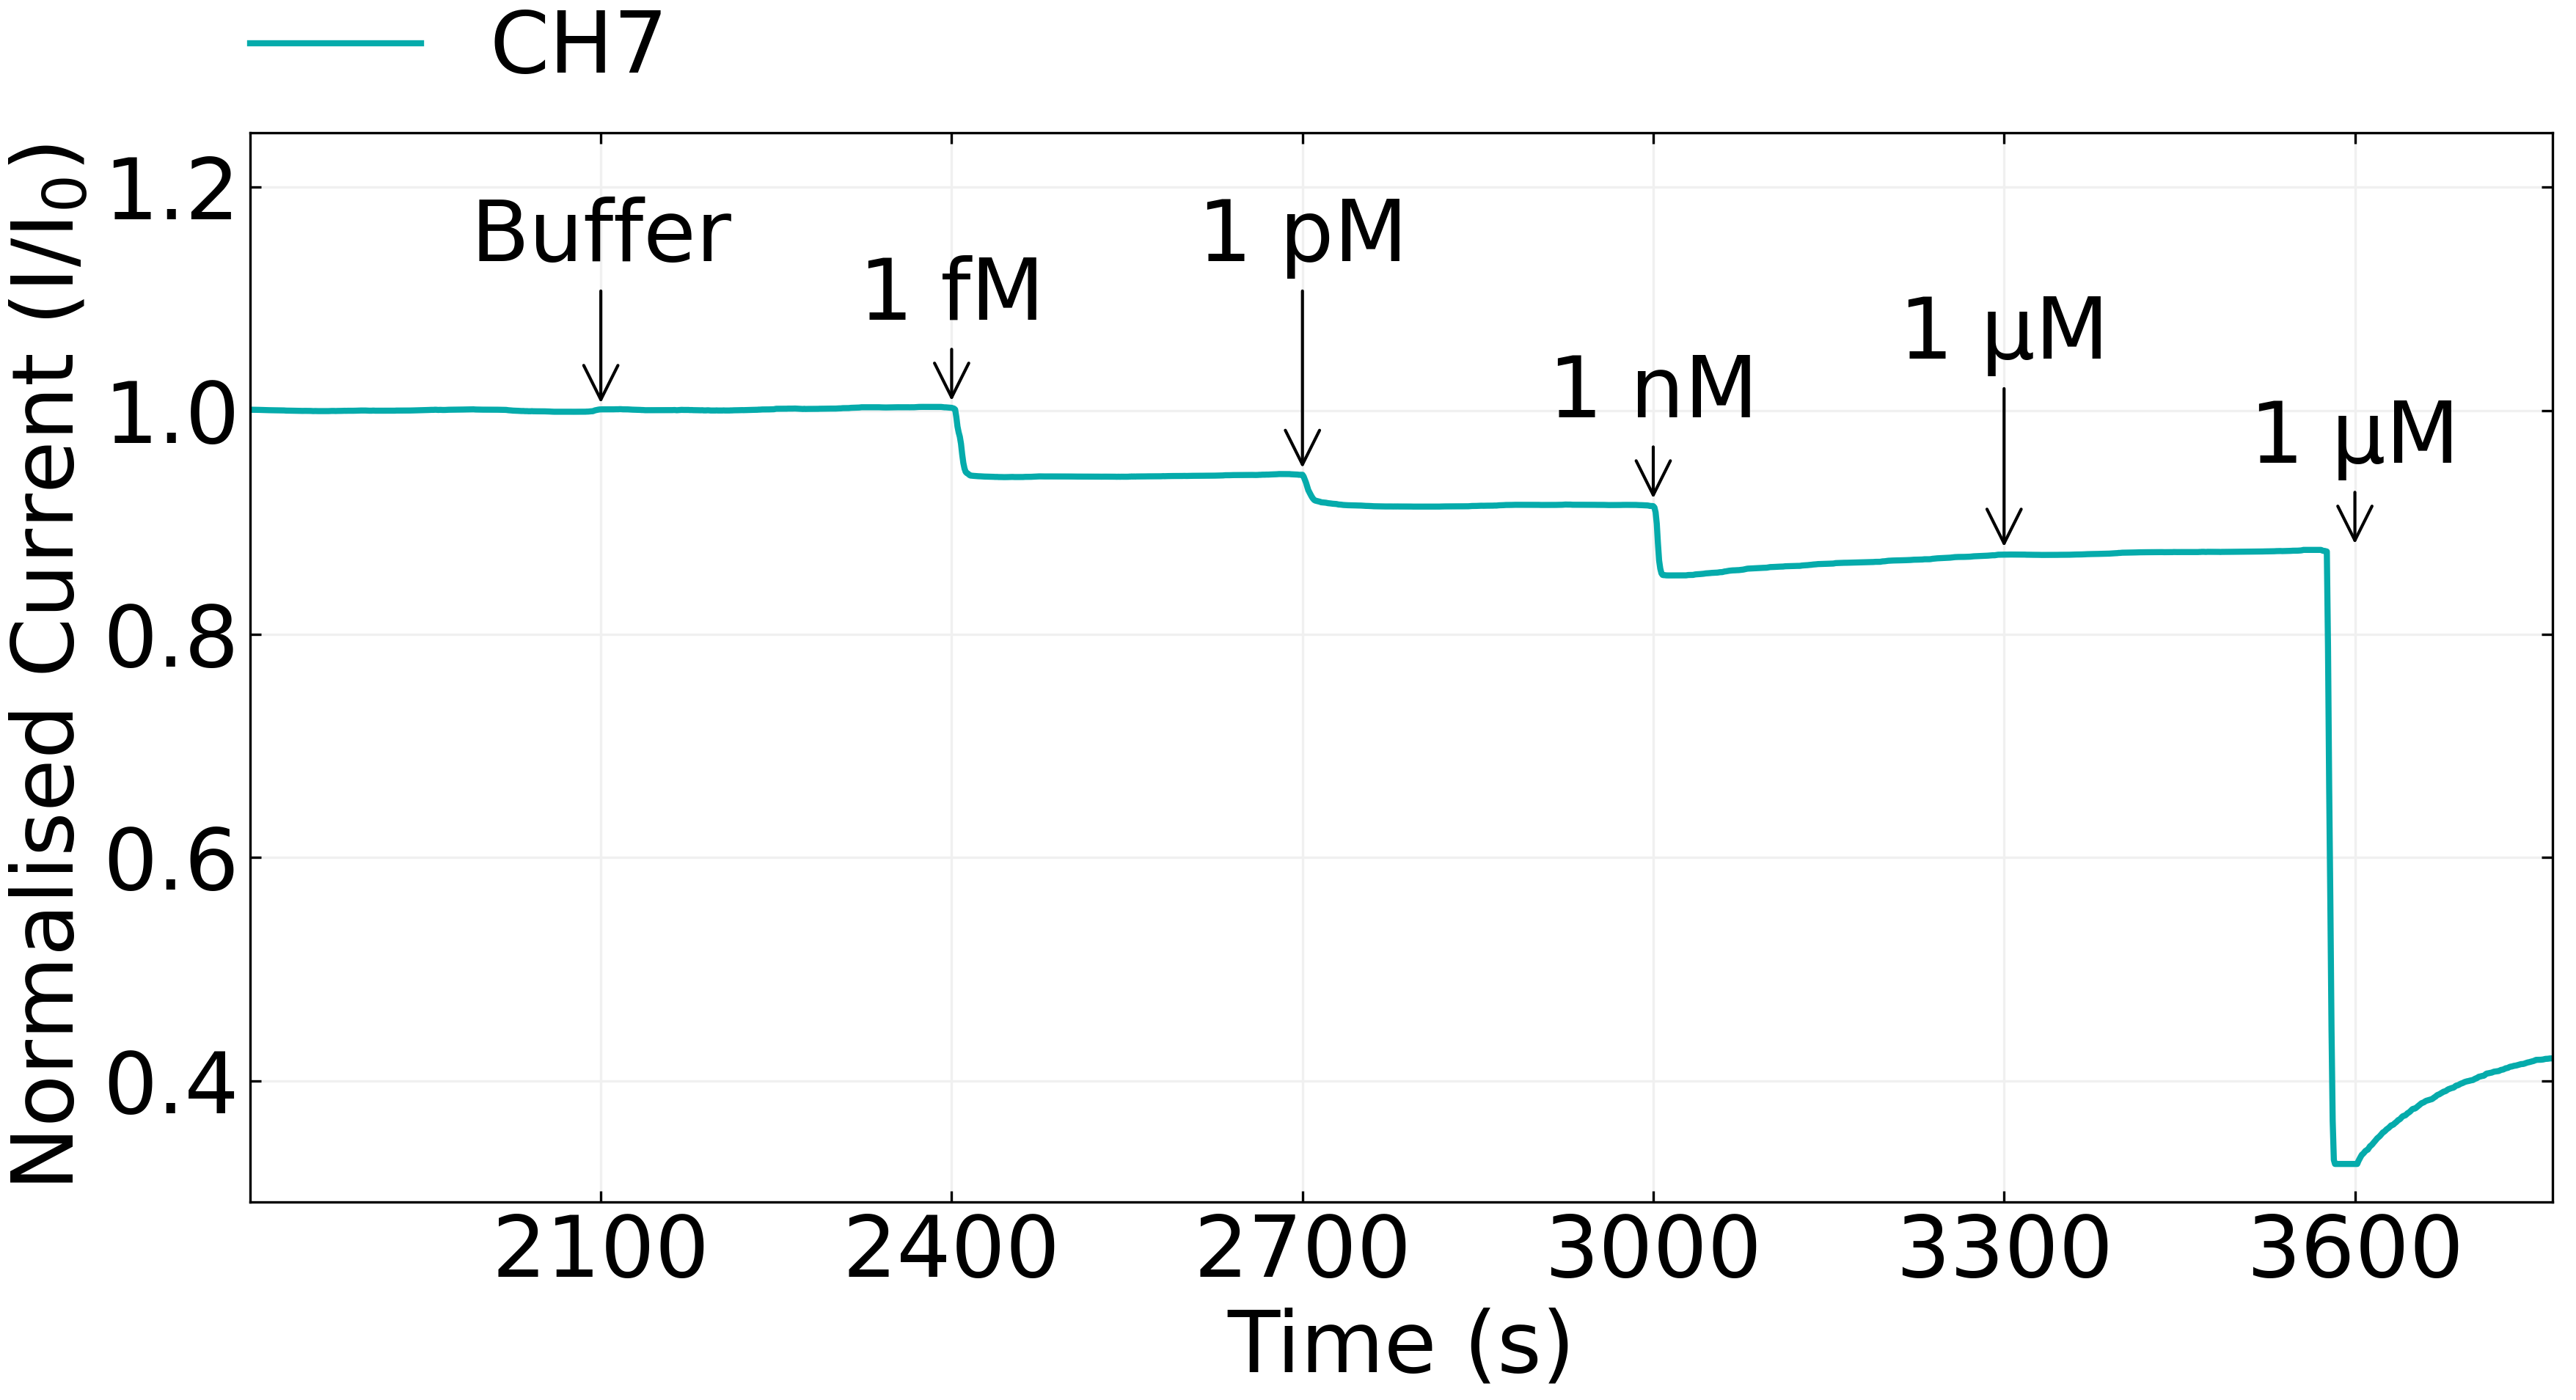
\includegraphics{figures/ch8/Q1C6_filtered_detrend_trunc_arrows_normalised.png}

}

}

\end{minipage}%
%
\begin{minipage}[t]{0.15\linewidth}

{\centering 

~

}

\end{minipage}%
\newline
\begin{minipage}[t]{0.11\linewidth}

{\centering 

~

}

\end{minipage}%
%
\begin{minipage}[t]{0.03\linewidth}

{\centering 

\raisebox{-\height}{

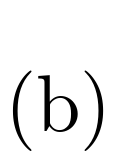
\includegraphics{figures/(b).png}

}

}

\end{minipage}%
%
\begin{minipage}[t]{0.01\linewidth}

{\centering 

~

}

\end{minipage}%
%
\begin{minipage}[t]{0.70\linewidth}

{\centering 

\raisebox{-\height}{

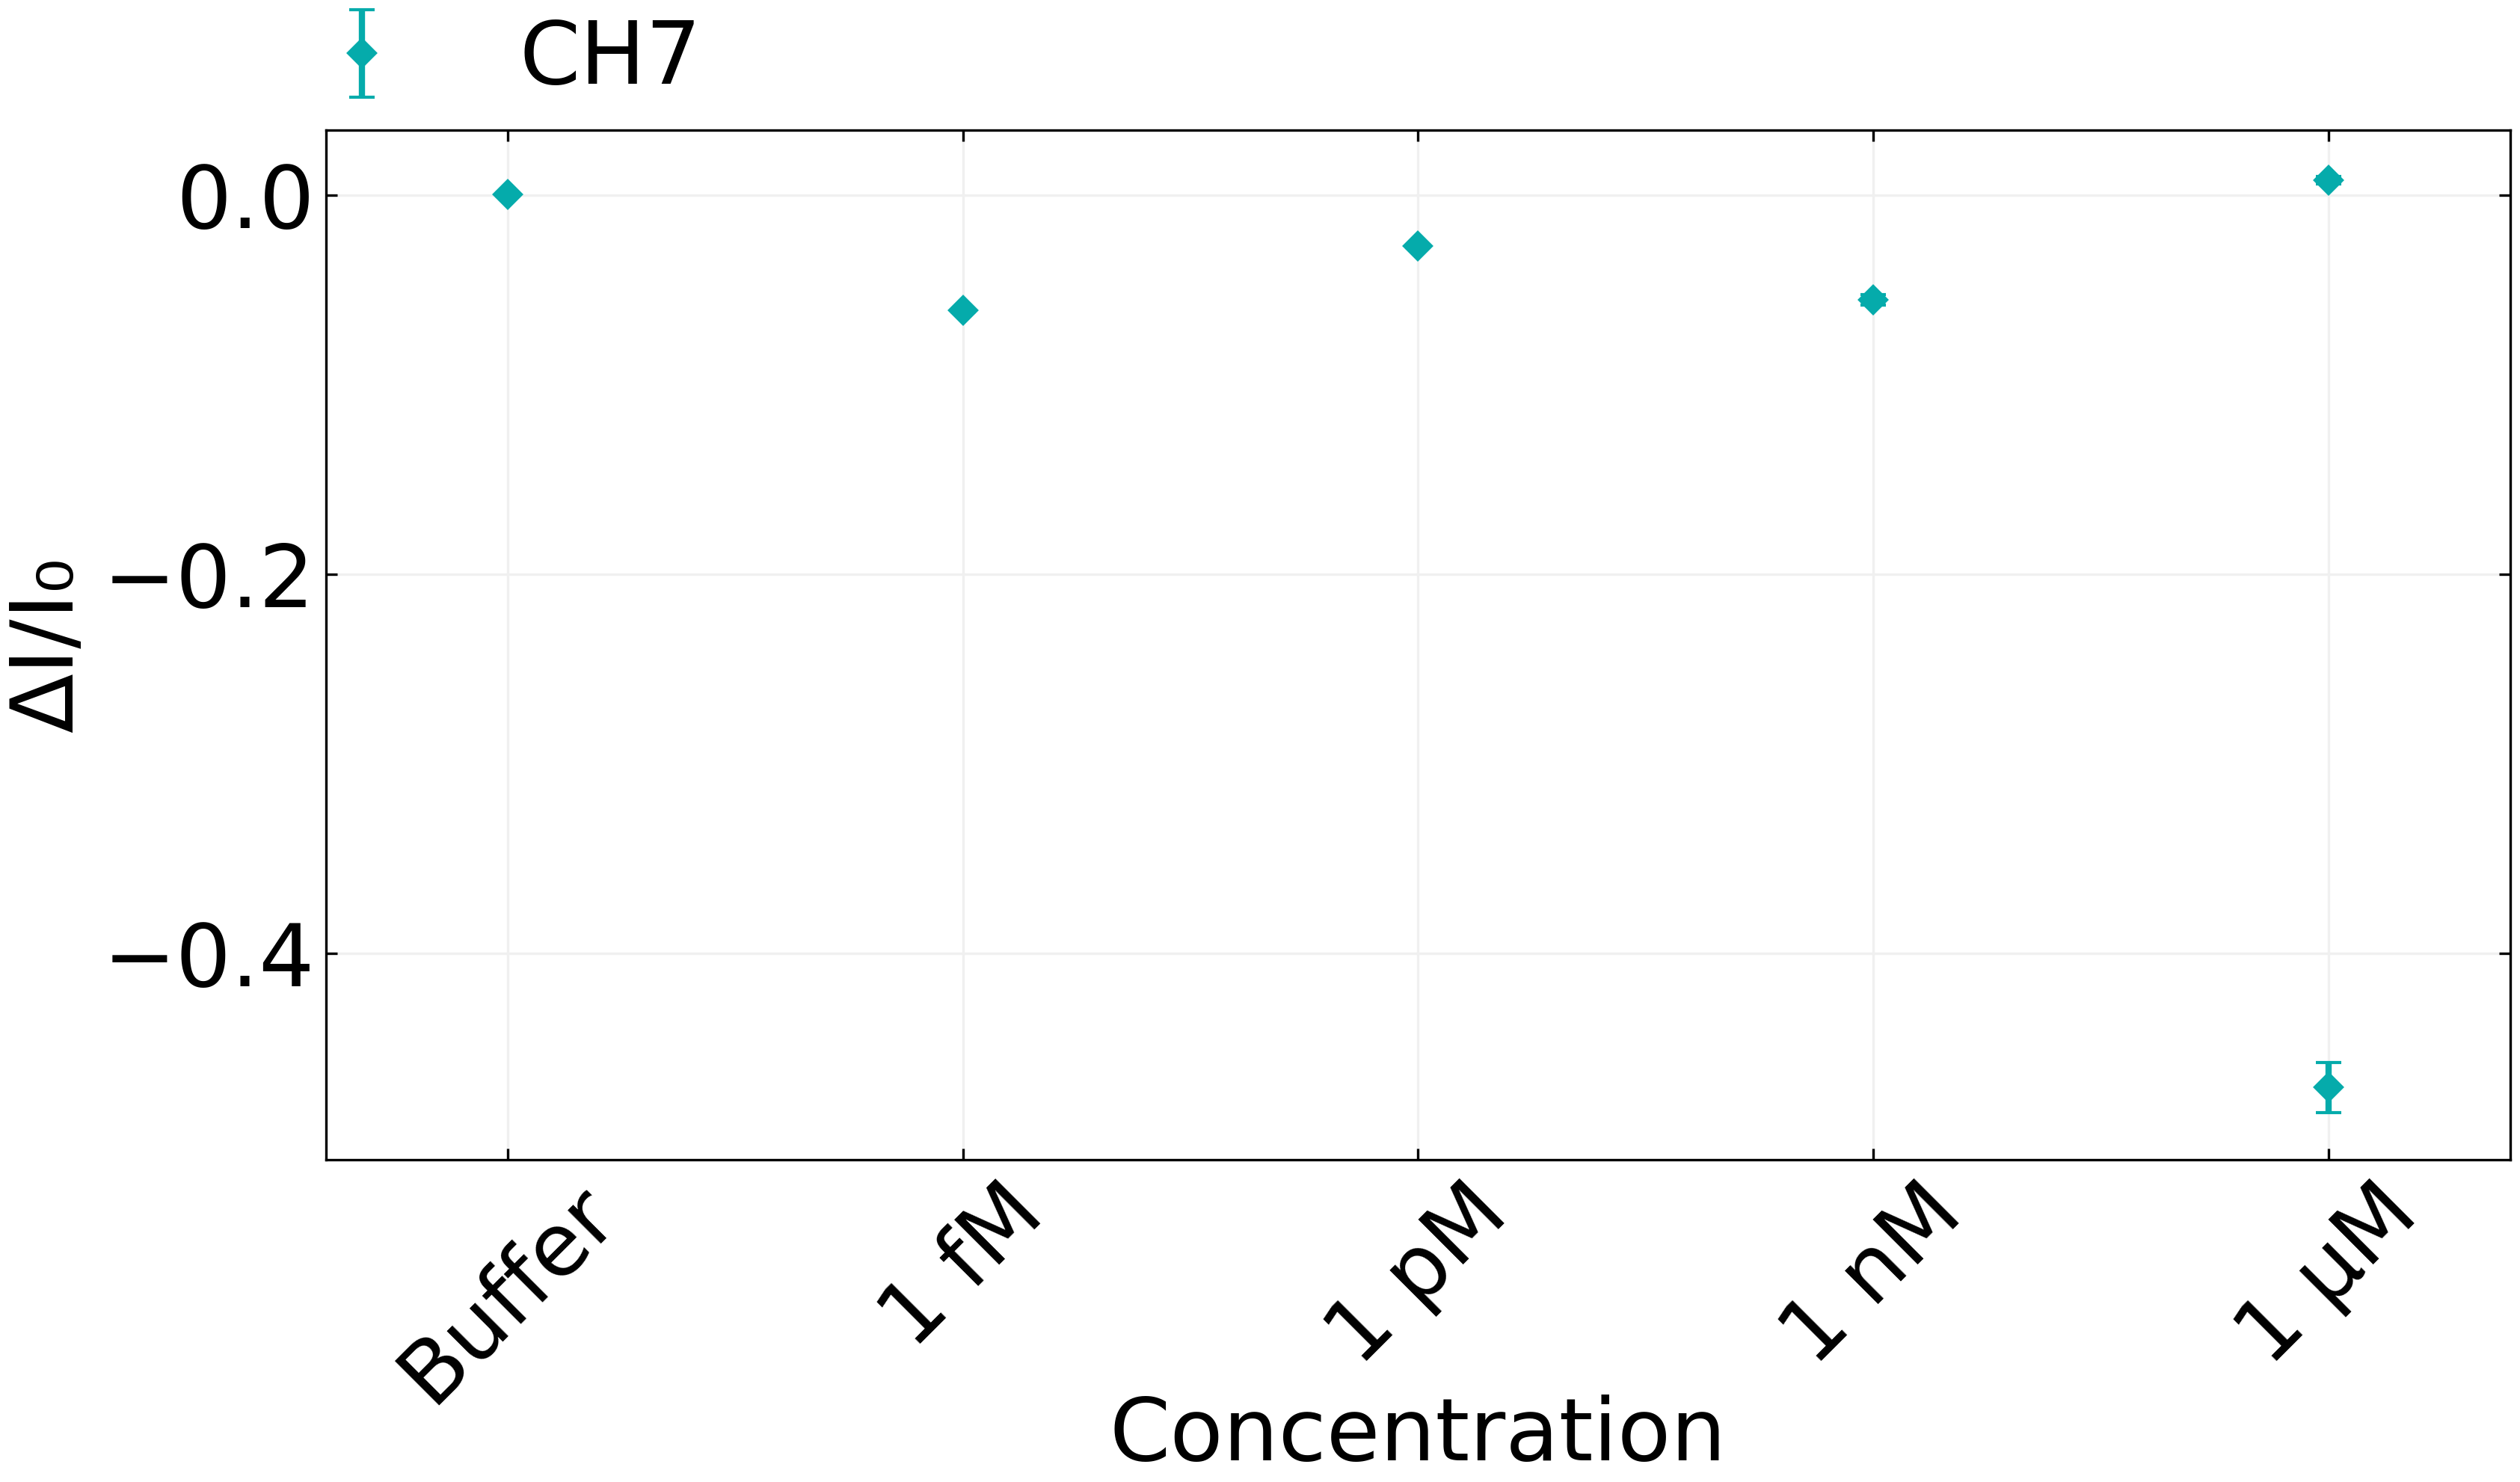
\includegraphics{figures/ch8/Q1C6_mean_simple_difference_before_and_after_step_filtered_concentrations.png}

}

}

\end{minipage}%
%
\begin{minipage}[t]{0.15\linewidth}

{\centering 

~

}

\end{minipage}%

\caption{\label{fig-OR22a-sensing-series}The normalised sensing series
for the OR22a-functionalised device is shown in (a). The current data
has been despiked, with baseline drift removed and a moving median
filter applied. The concentration of each 20 µL addition is indicated
above the time of addition. The signal data corresponding to the mean
difference in current before and after each addition is shown in (b).}

\end{figure}

Figure~\ref{fig-OR22a-sensing-series} (a) shows the cleaned and filtered
ethyl hexanoate sensing data from the OR22a-functionalised device from
1800 s onwards. The concentration of each 20 µL addition is indicated
above the corresponding addition time. The source-drain current across
the channel decreased rapidly with each addition of ethyl hexanoate in
\(0.5%
\) DMSO 1XPBS solution. This current decrease appears irreversible, as
the current stabilises after each addition at a lower current level than
prior to the addition. This behaviour appears to be a response by OR22a
to its positive ligand ethyl hexanoate, similar to the response by OR22a
to methyl hexanoate seen by Murugathas \emph{et al.}. The presence of
the ORCO coreceptor was not required for responses to be seen. The
device showed responses to ethyl hexanoate over a wide range of
concentrations, beginning with a \(\sim 6\)\% response to 1 fM EtHex in
\(0.5%
\) DMSO 1XPBS, while showing no response to 0.5\% 1XPBS buffer.
Interestingly, as seen in Figure~\ref{fig-OR22a-sensing-series} (b), no
clear dose-dependent response was observed. The behaviour seen may be
explained by a decreased sensitivity to subsequent additions seen by
seen by Murugathas \emph{et al.} \autocite{Murugathas2019b} competing
with the logarithmic increases in the concentration around the channel.

\hypertarget{sec-variability}{%
\section{Addressing Biosensor Variability}\label{sec-variability}}

\hypertarget{sec-variability-biosensor}{%
\subsection{Variability in Biosensor
Behaviour}\label{sec-variability-biosensor}}

\begin{figure}

\begin{minipage}[t]{0.11\linewidth}

{\centering 

~

}

\end{minipage}%
%
\begin{minipage}[t]{0.03\linewidth}

{\centering 

\raisebox{-\height}{


\includegraphics{figures/(a).png}

}

}

\end{minipage}%
%
\begin{minipage}[t]{0.01\linewidth}

{\centering 

~

}

\end{minipage}%
%
\begin{minipage}[t]{0.70\linewidth}

{\centering 

\raisebox{-\height}{

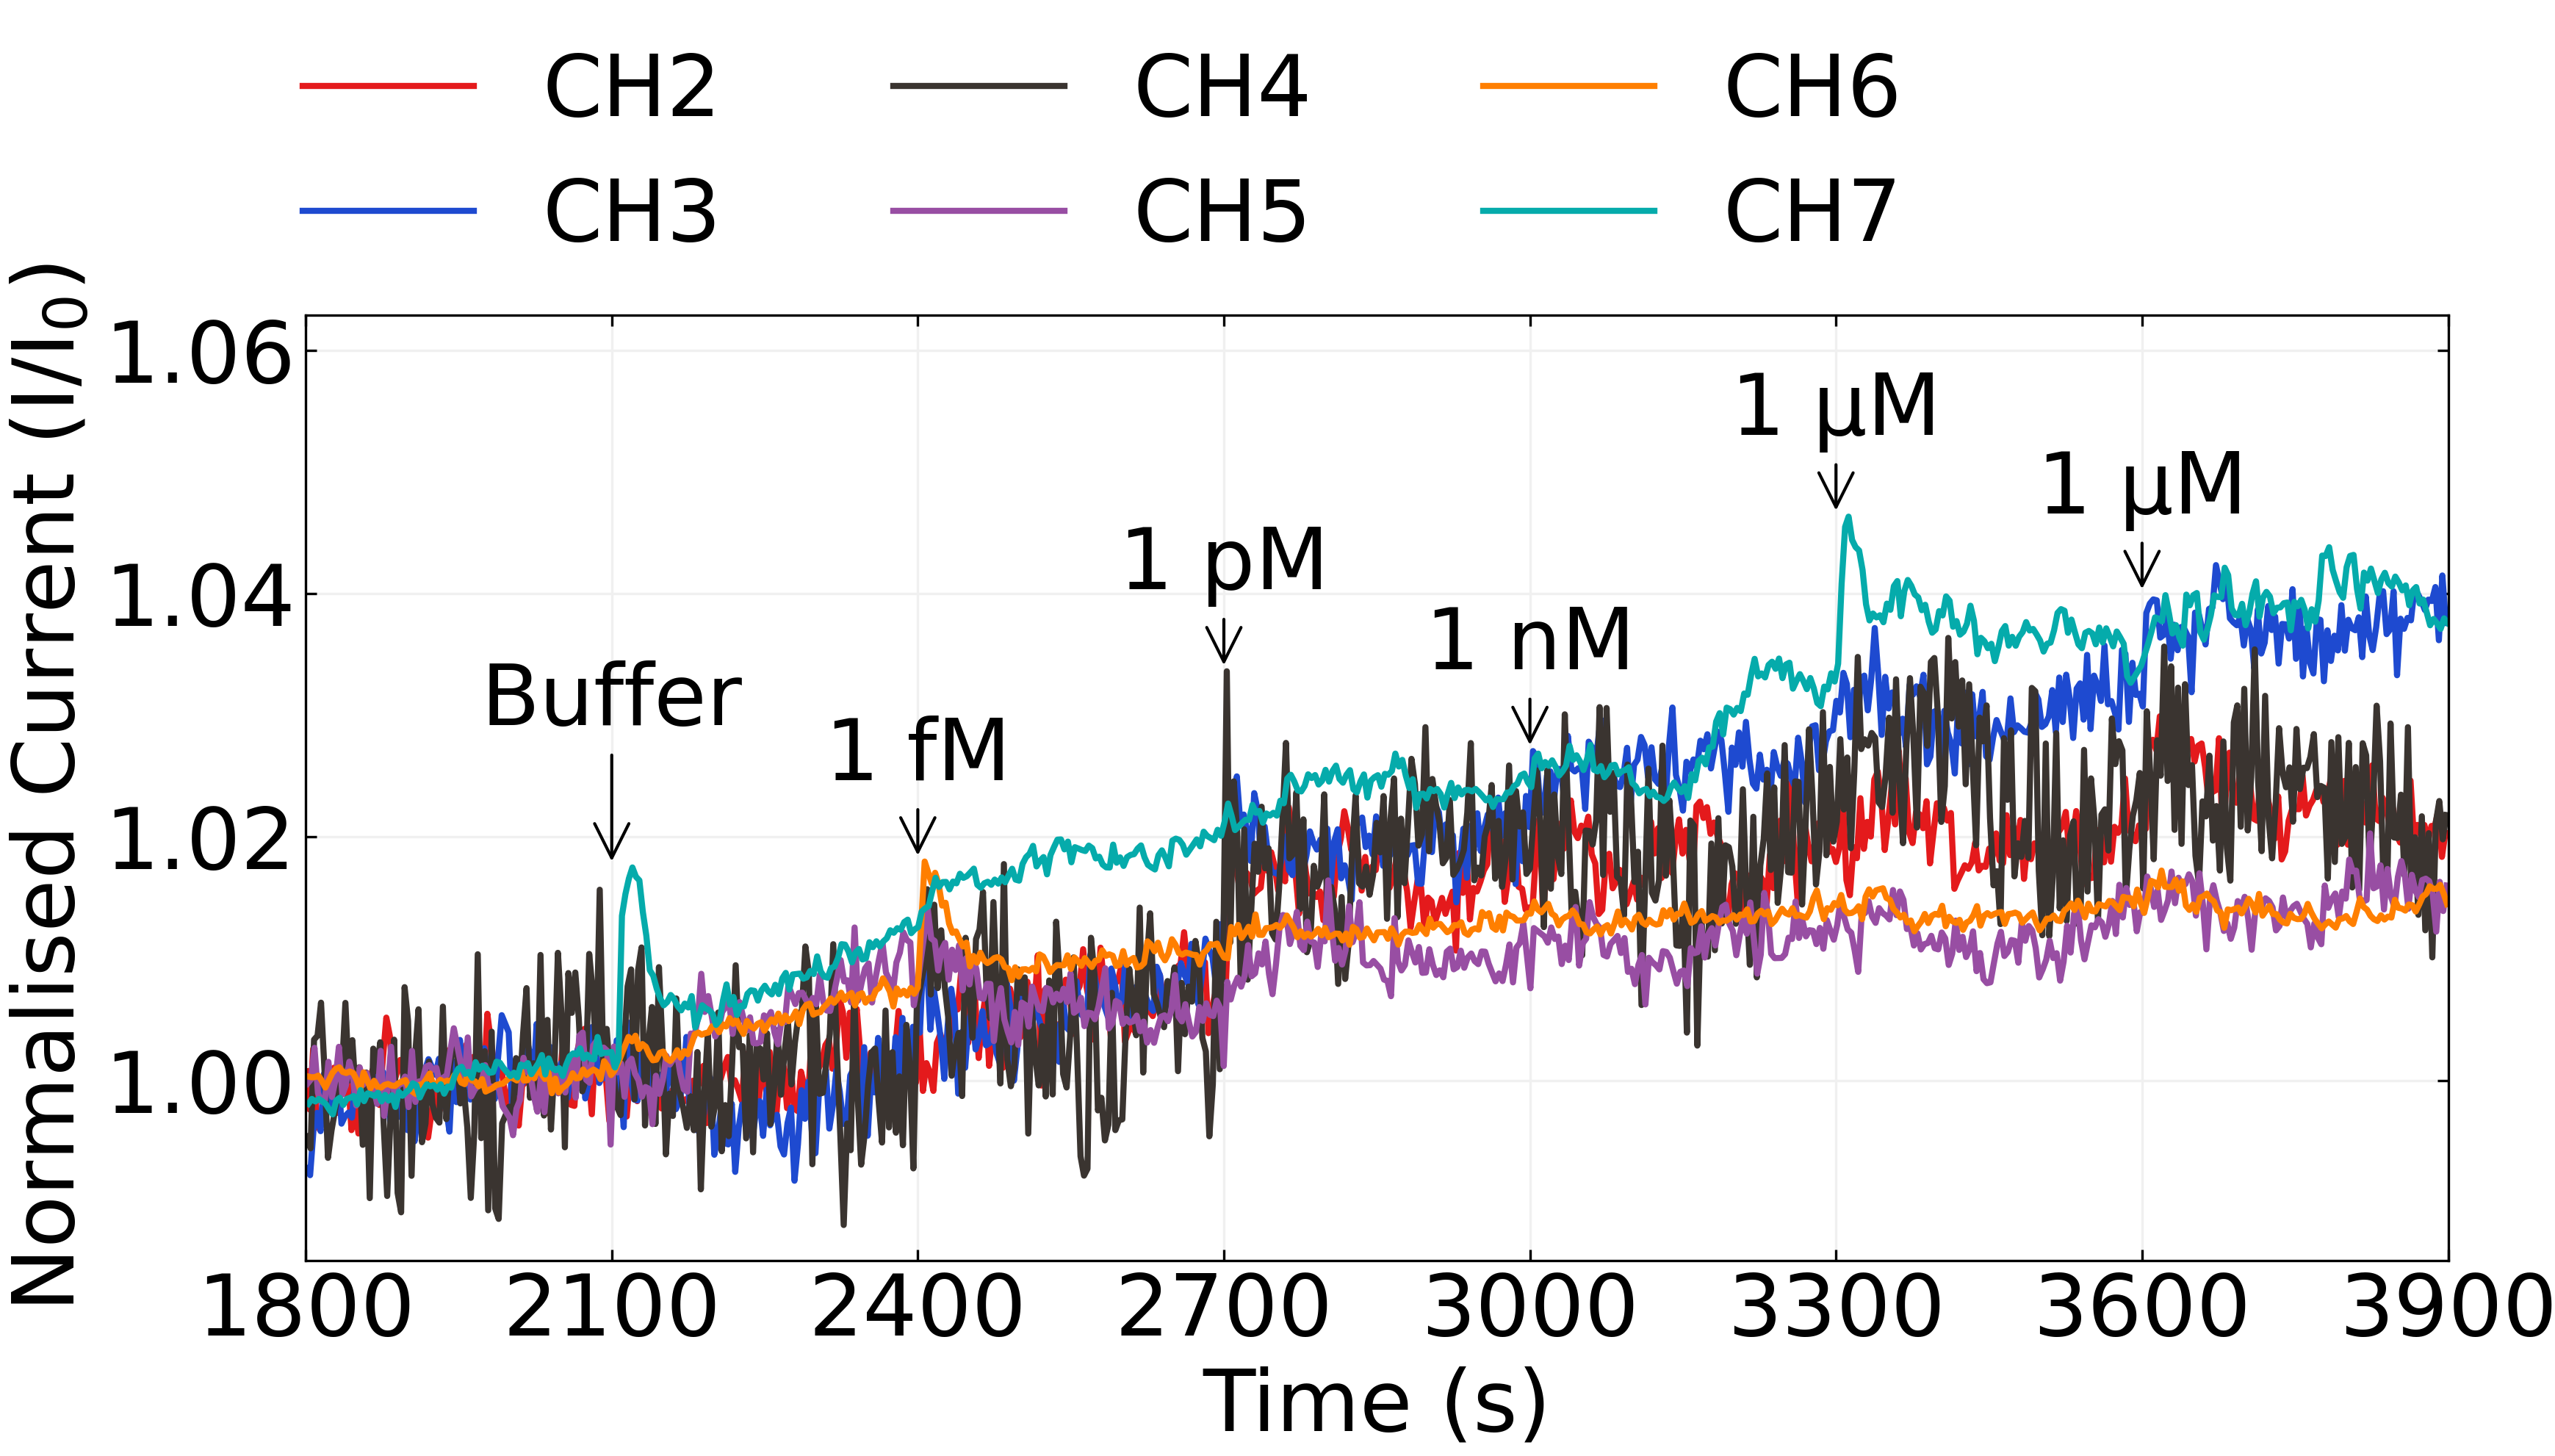
\includegraphics{figures/ch8/Q4C4_OR22a_Functionalised_2ndTimeSensingRun_48hrFridge_21_detrend_trunc_arrows_normalised.png}

}

}

\end{minipage}%
%
\begin{minipage}[t]{0.15\linewidth}

{\centering 

~

}

\end{minipage}%
\newline
\begin{minipage}[t]{0.11\linewidth}

{\centering 

~

}

\end{minipage}%
%
\begin{minipage}[t]{0.03\linewidth}

{\centering 

\raisebox{-\height}{

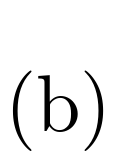
\includegraphics{figures/(b).png}

}

}

\end{minipage}%
%
\begin{minipage}[t]{0.01\linewidth}

{\centering 

~

}

\end{minipage}%
%
\begin{minipage}[t]{0.70\linewidth}

{\centering 

\raisebox{-\height}{

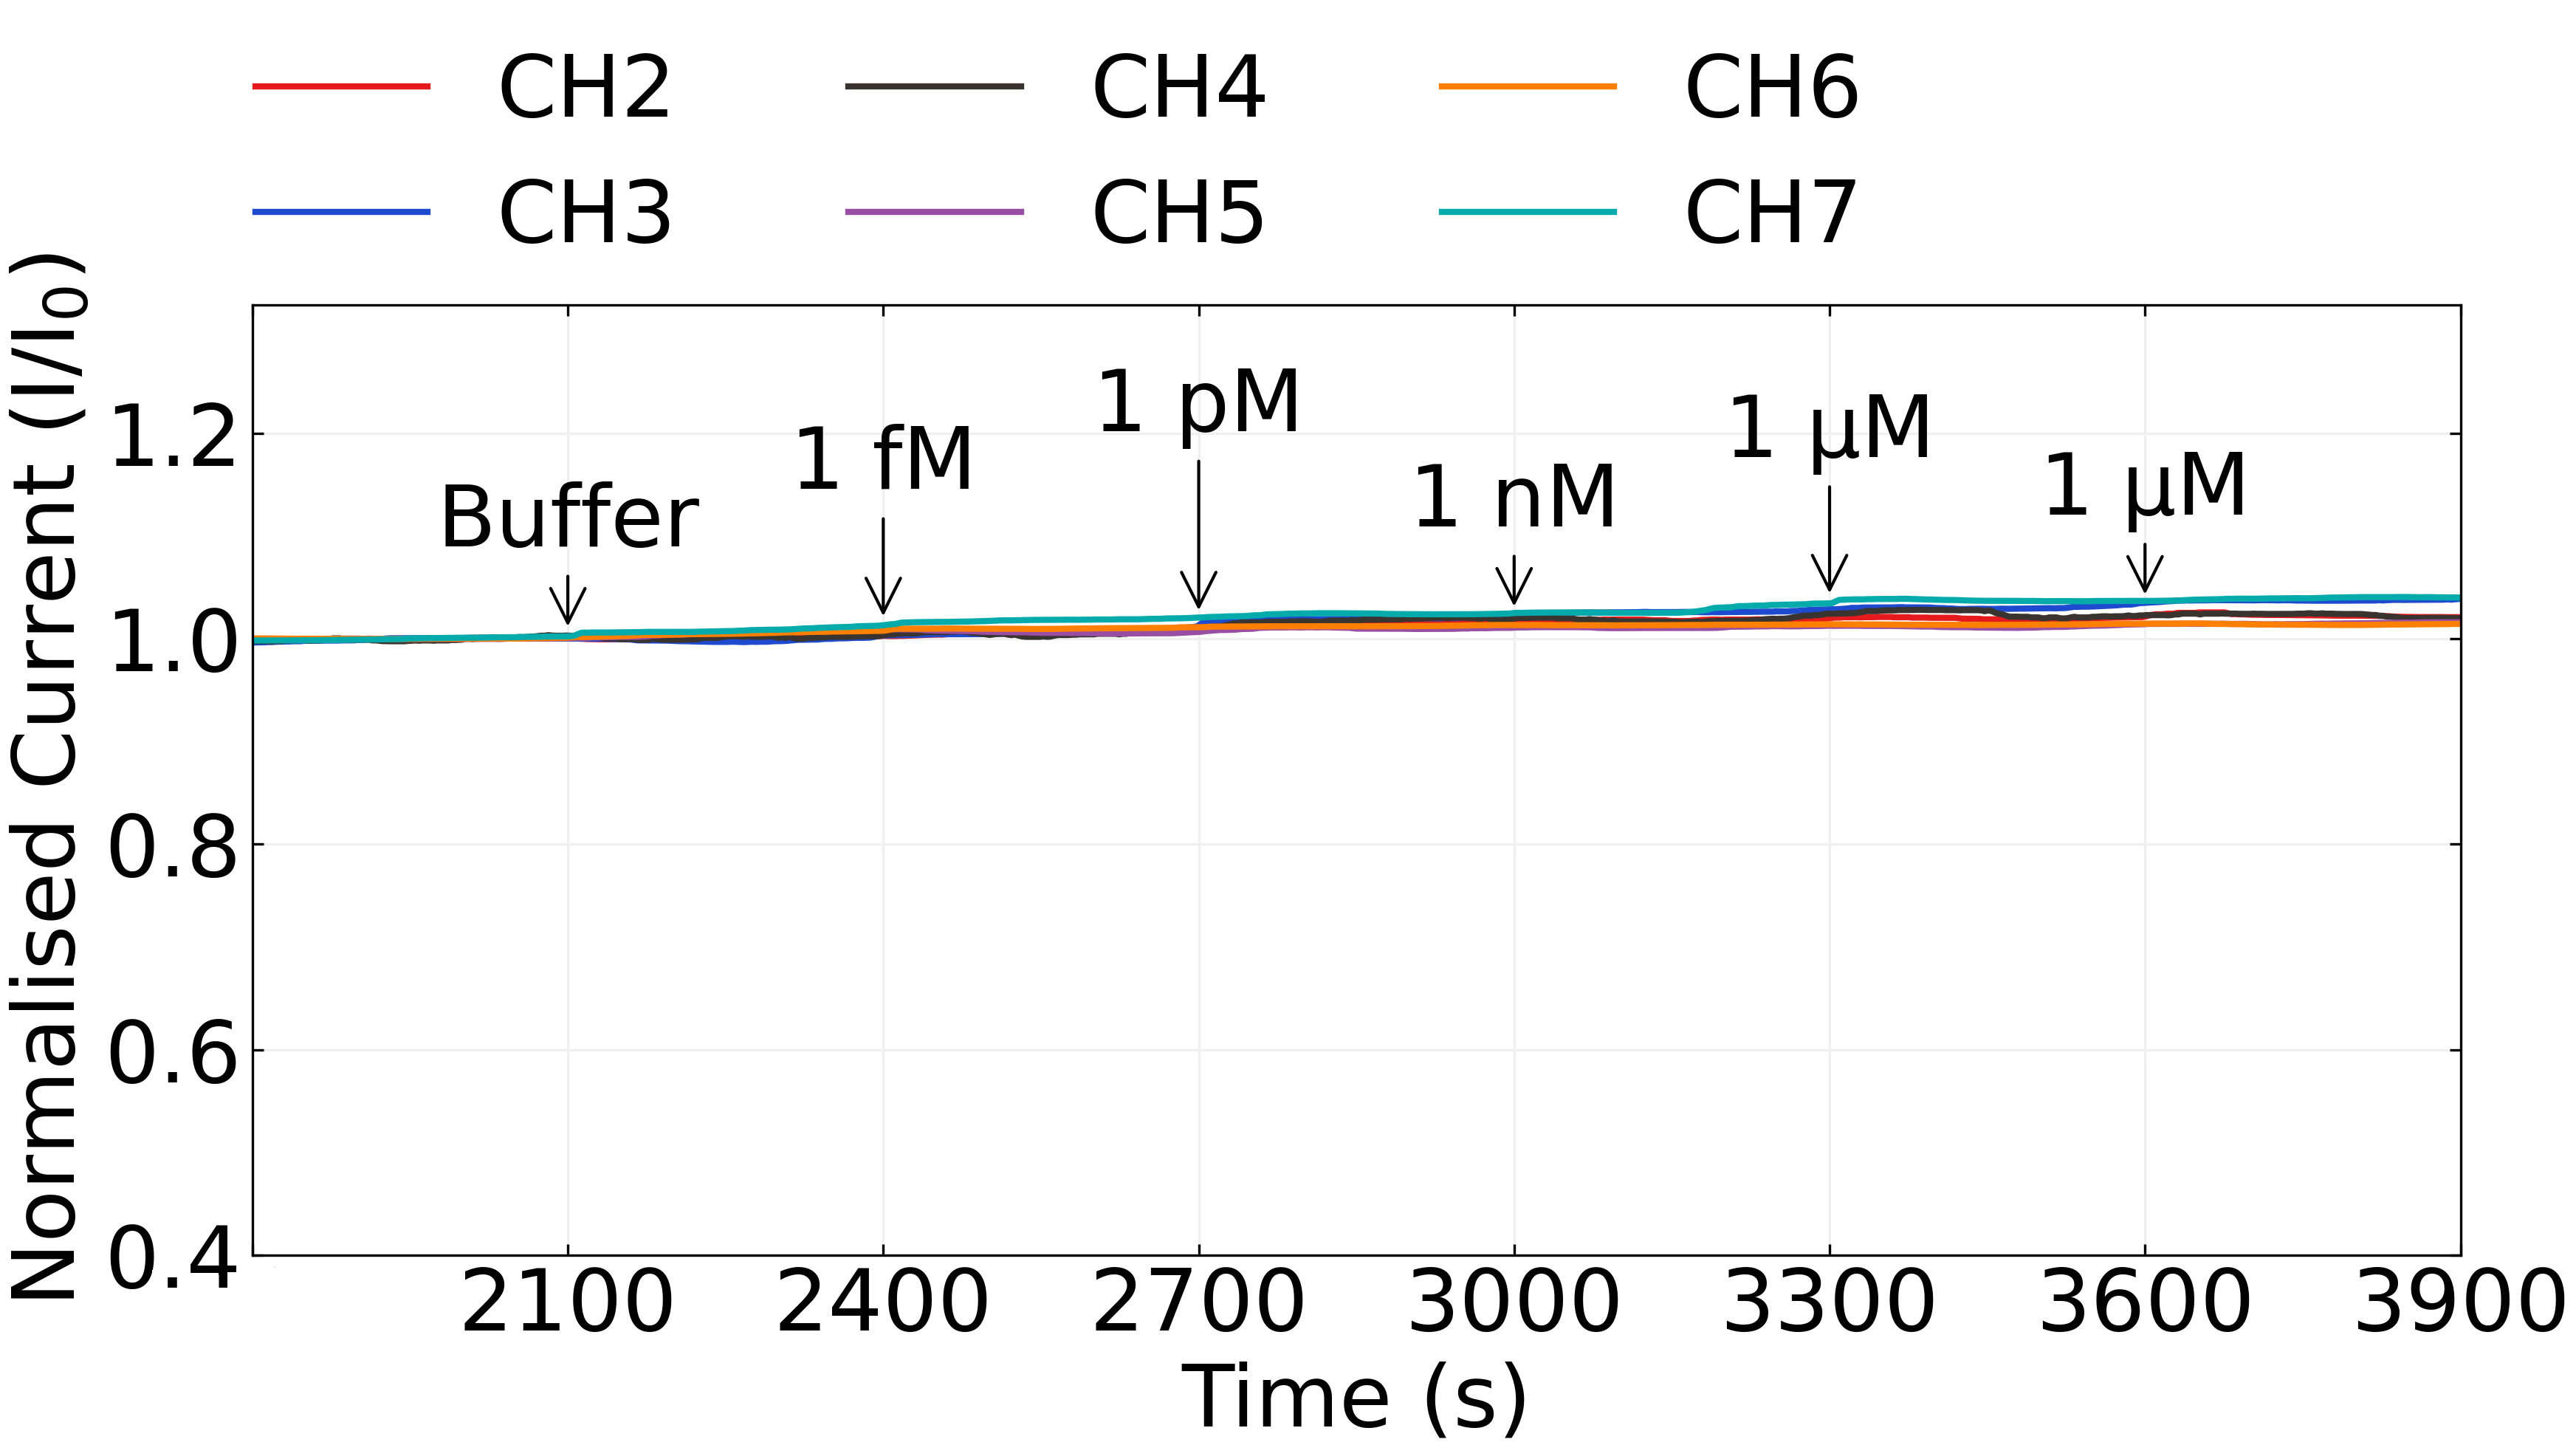
\includegraphics{figures/ch8/Q4C4_OR22a_Functionalised_2ndTimeSensingRun_48hrFridge_21_filtered_detrend_trunc_arrows_normalised.png}

}

}

\end{minipage}%
%
\begin{minipage}[t]{0.15\linewidth}

{\centering 

~

}

\end{minipage}%

\caption{\label{fig-OR22a-variability}The normalised sensing series of
another OR22a-functionalised device across six multiplexed channels,
where current data has been despiked and baseline drift removed. The
concentration of each 20 µL addition is indicated above the time of
addition. The same sensing series is shown in both (a) and (b), where a
moving median filter has been applied in (b).}

\end{figure}

Despite the successful detection of ethyl hexanoate by an OR22a
nanodisc-functionalised biosensor in
Section~\ref{sec-aqueous-sensing-EtHex}, it was found that this
behaviour was not readily reproducible. The results from the previous
section were not repeated when using the same procedure for fabrication
of devices alongside an identical functionalisation process with the
same batch of OR22a nanodiscs (ND-OR22a-SB018). The ethyl hexanoate
sensing sequence from six functionalised device channels is shown in
Figure~\ref{fig-OR22a-variability}. Figure~\ref{fig-OR22a-variability}
(a) has been left unfiltered to illustrate the variation in behaviour
between channels, while Figure~\ref{fig-OR22a-variability} (b) has been
prepared in the same manner as Figure~\ref{fig-OR22a-sensing-series}
(a). The current response to each analyte addition is similar to that
seen after the initial addition without ethyl hexanoate present. The
largest contributing factor to current change appears to be drift.
Unlike the clear decreases in current subsequent to ethyl hexanoate
additions seen in Figure~\ref{fig-OR22a-sensing-series} (a), no
decreases are seen in Figure~\ref{fig-OR22a-variability} (b) to any
ethyl hexanoate solution addition.

\begin{figure}

\begin{minipage}[t]{0.03\linewidth}

{\centering 

\raisebox{-\height}{


\includegraphics{figures/(a).png}

}

}

\end{minipage}%
%
\begin{minipage}[t]{0.01\linewidth}

{\centering 

~

}

\end{minipage}%
%
\begin{minipage}[t]{0.45\linewidth}

{\centering 

\raisebox{-\height}{

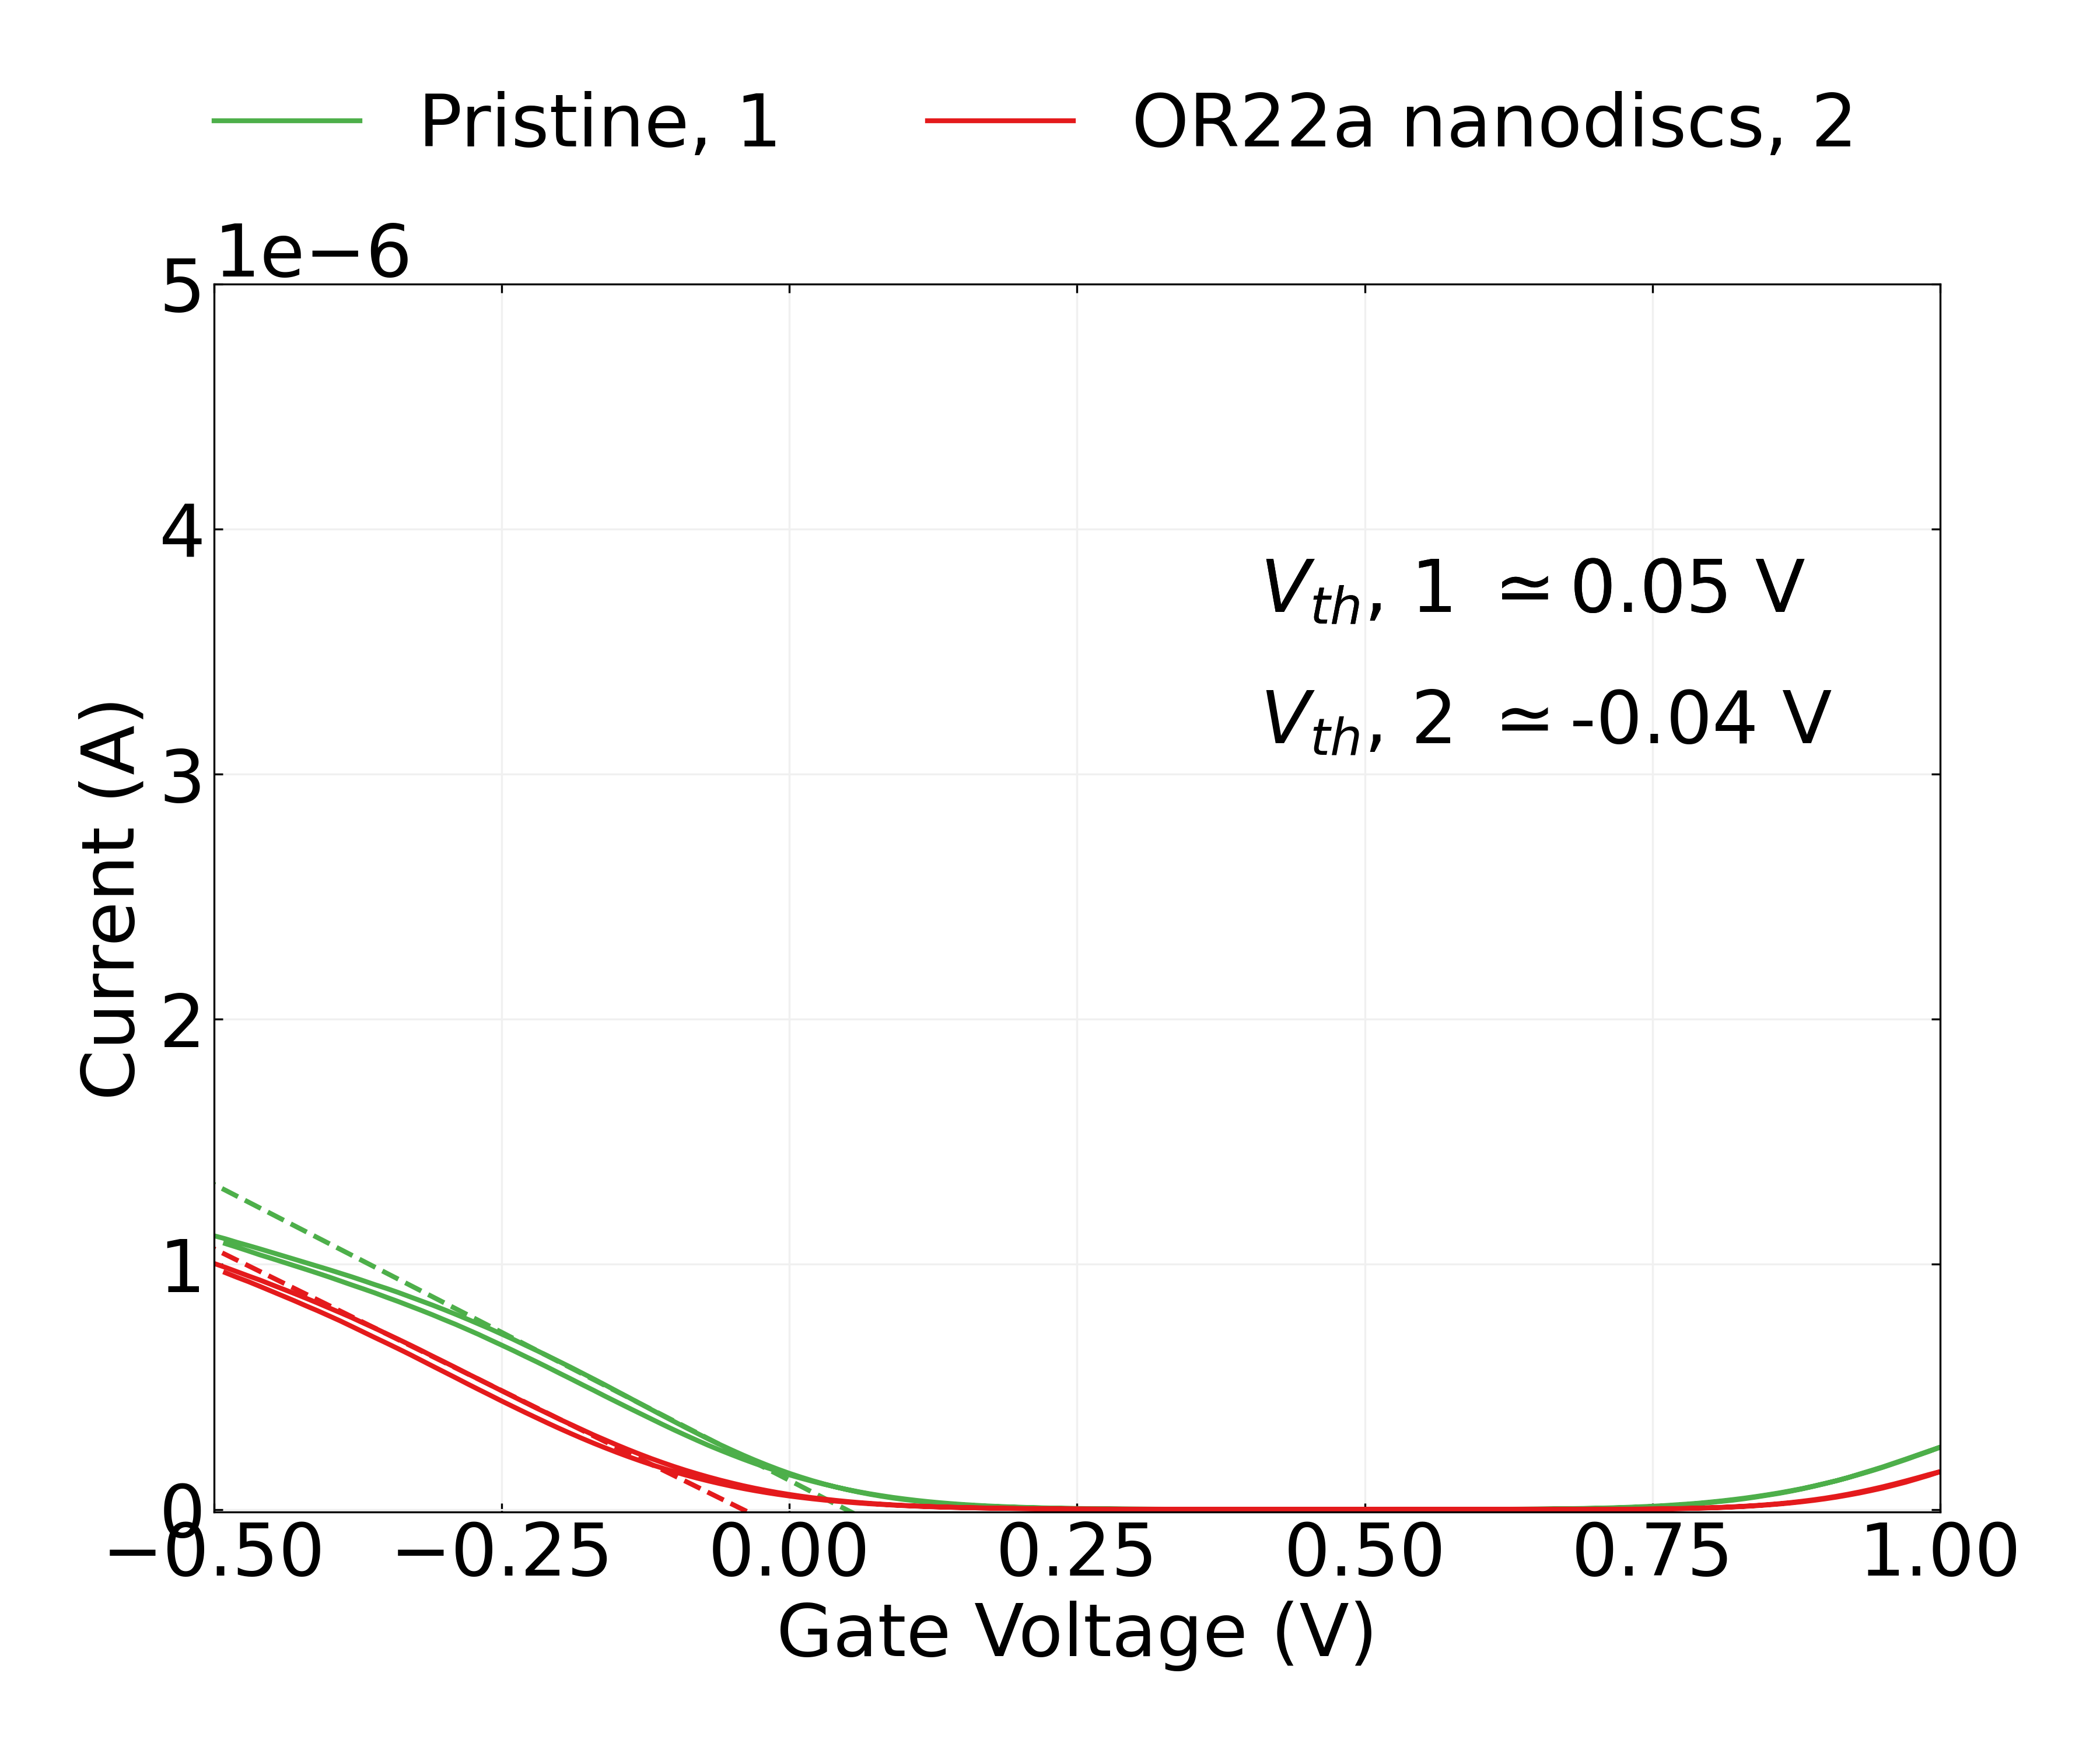
\includegraphics{figures/ch8/Q4C4_ch2.png}

}

}

\end{minipage}%
%
\begin{minipage}[t]{0.01\linewidth}

{\centering 

~

}

\end{minipage}%
%
\begin{minipage}[t]{0.03\linewidth}

{\centering 

\raisebox{-\height}{

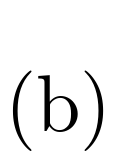
\includegraphics{figures/(b).png}

}

}

\end{minipage}%
%
\begin{minipage}[t]{0.01\linewidth}

{\centering 

~

}

\end{minipage}%
%
\begin{minipage}[t]{0.45\linewidth}

{\centering 

\raisebox{-\height}{

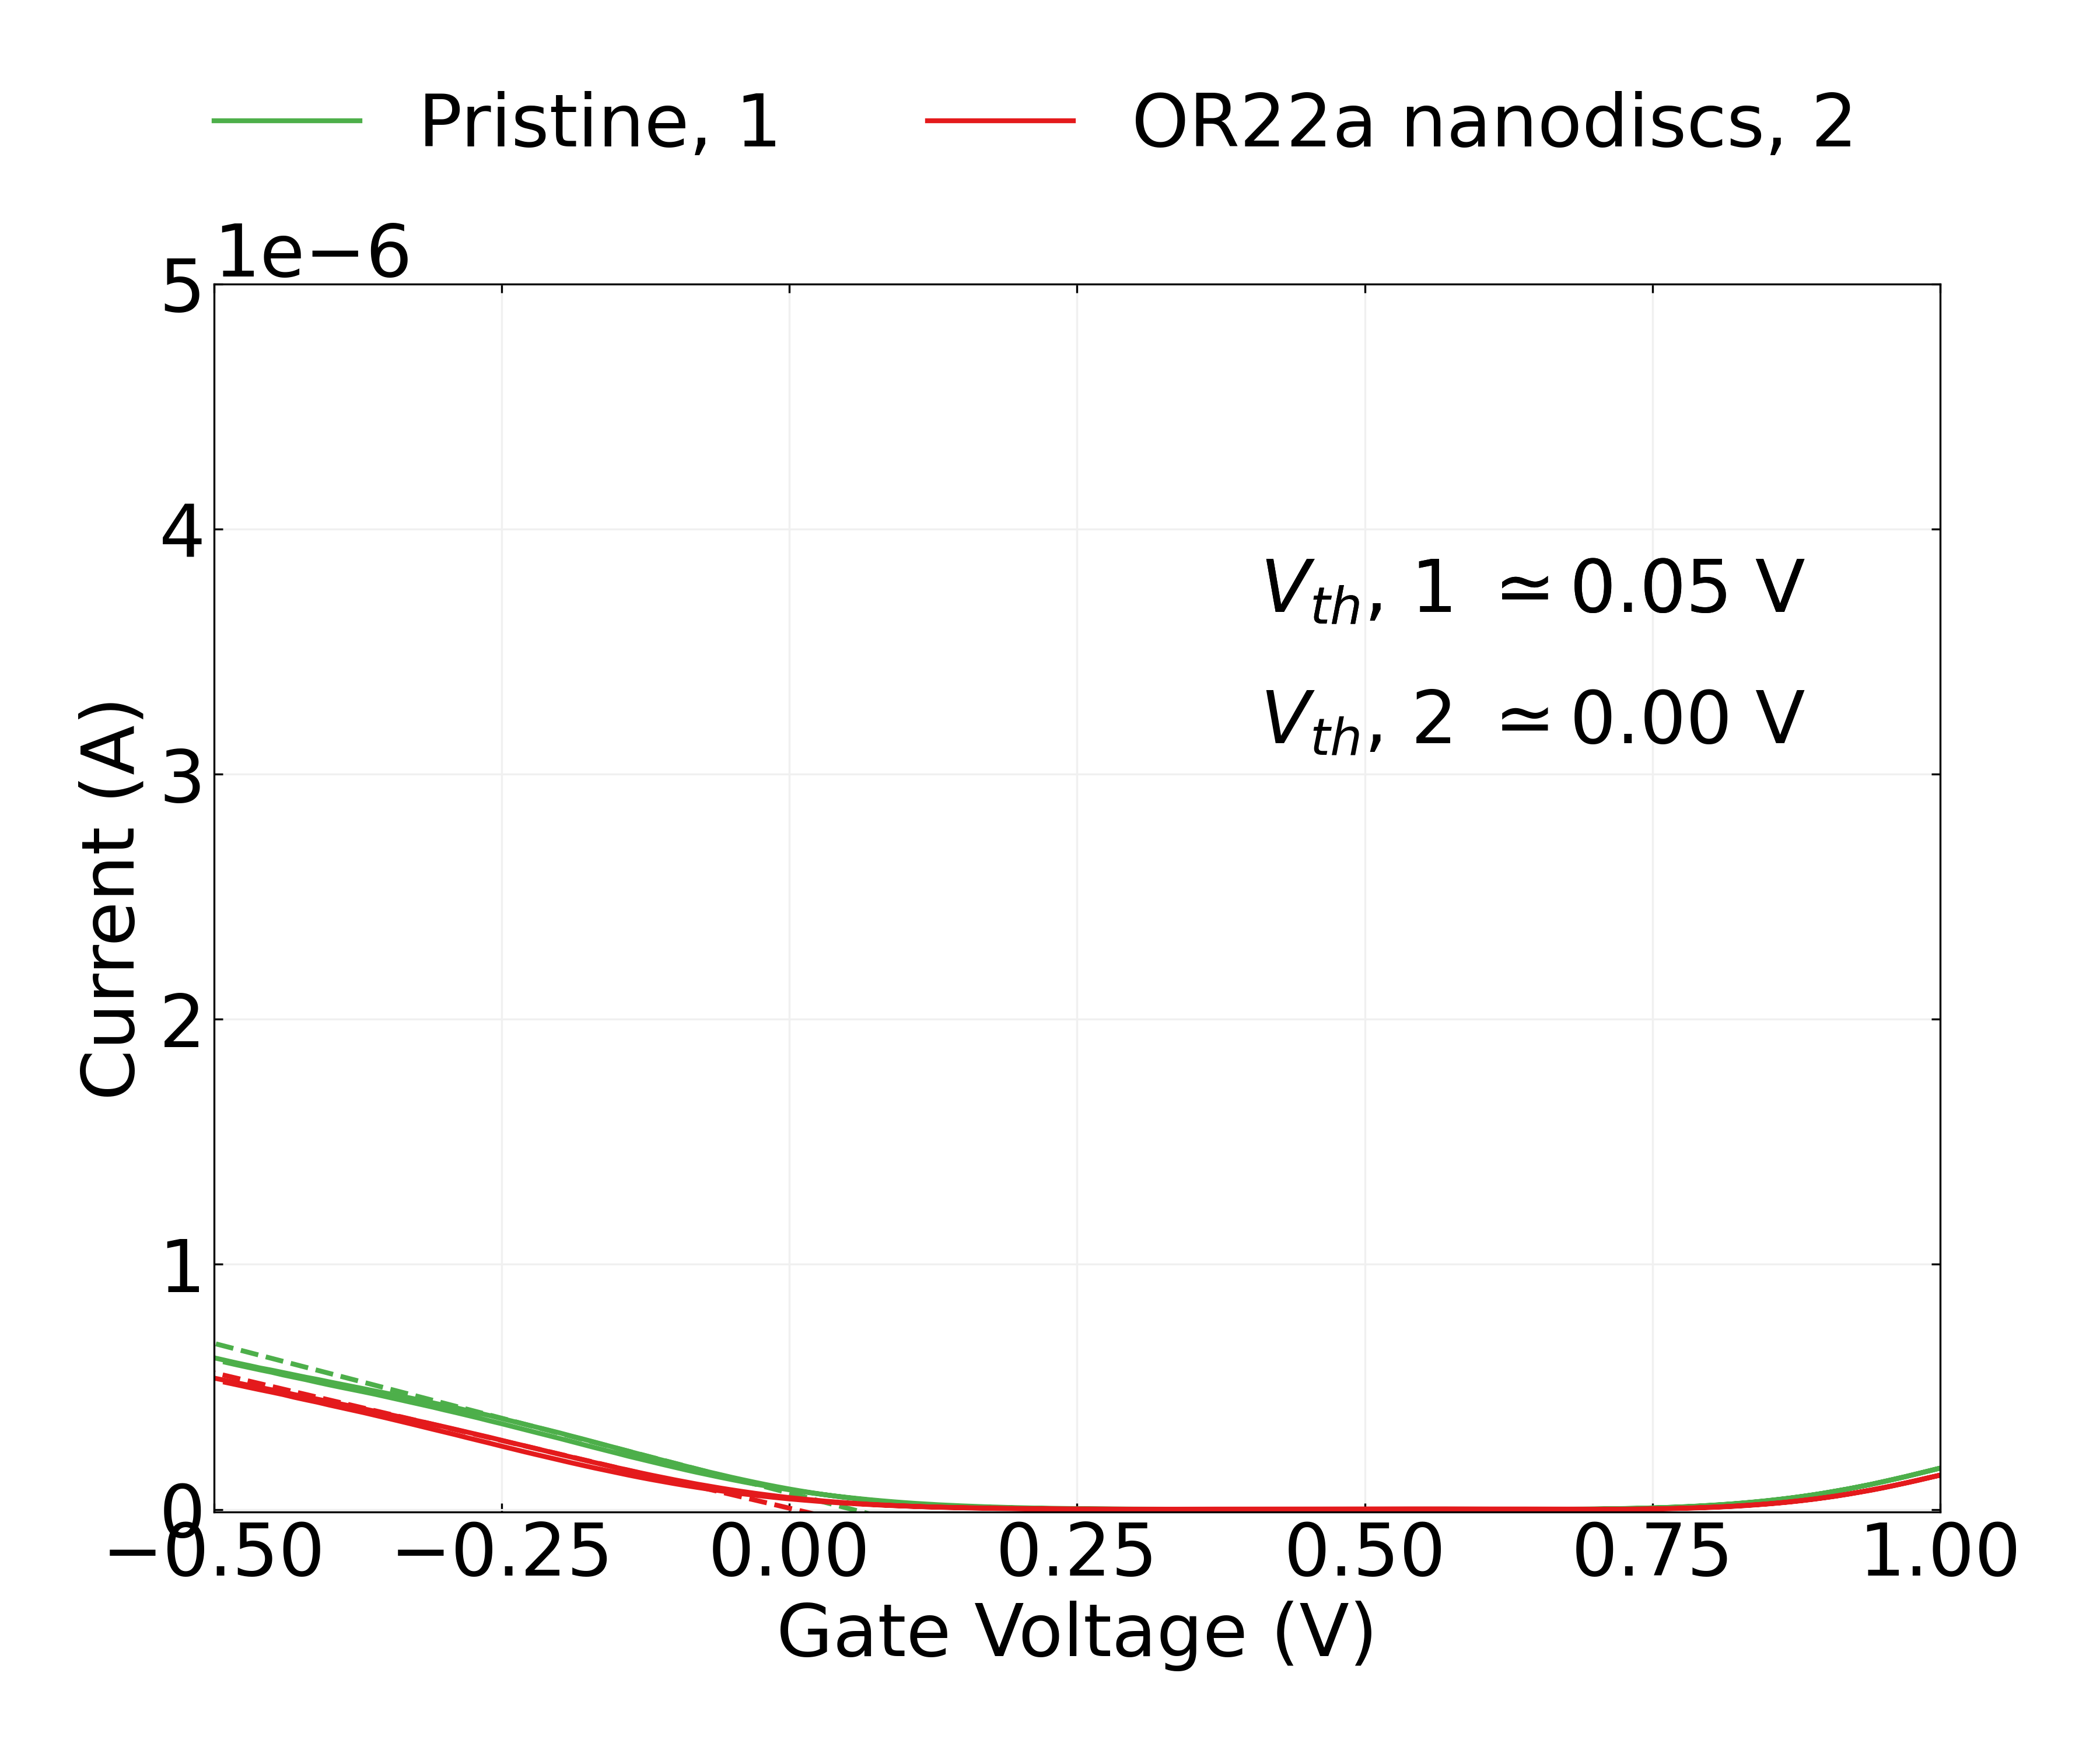
\includegraphics{figures/ch8/Q4C4_ch3.png}

}

}

\end{minipage}%
%
\begin{minipage}[t]{0.01\linewidth}

{\centering 

~

}

\end{minipage}%
\newline
\begin{minipage}[t]{0.03\linewidth}

{\centering 

\raisebox{-\height}{


\includegraphics{figures/(c).png}

}

}

\end{minipage}%
%
\begin{minipage}[t]{0.01\linewidth}

{\centering 

~

}

\end{minipage}%
%
\begin{minipage}[t]{0.45\linewidth}

{\centering 

\raisebox{-\height}{

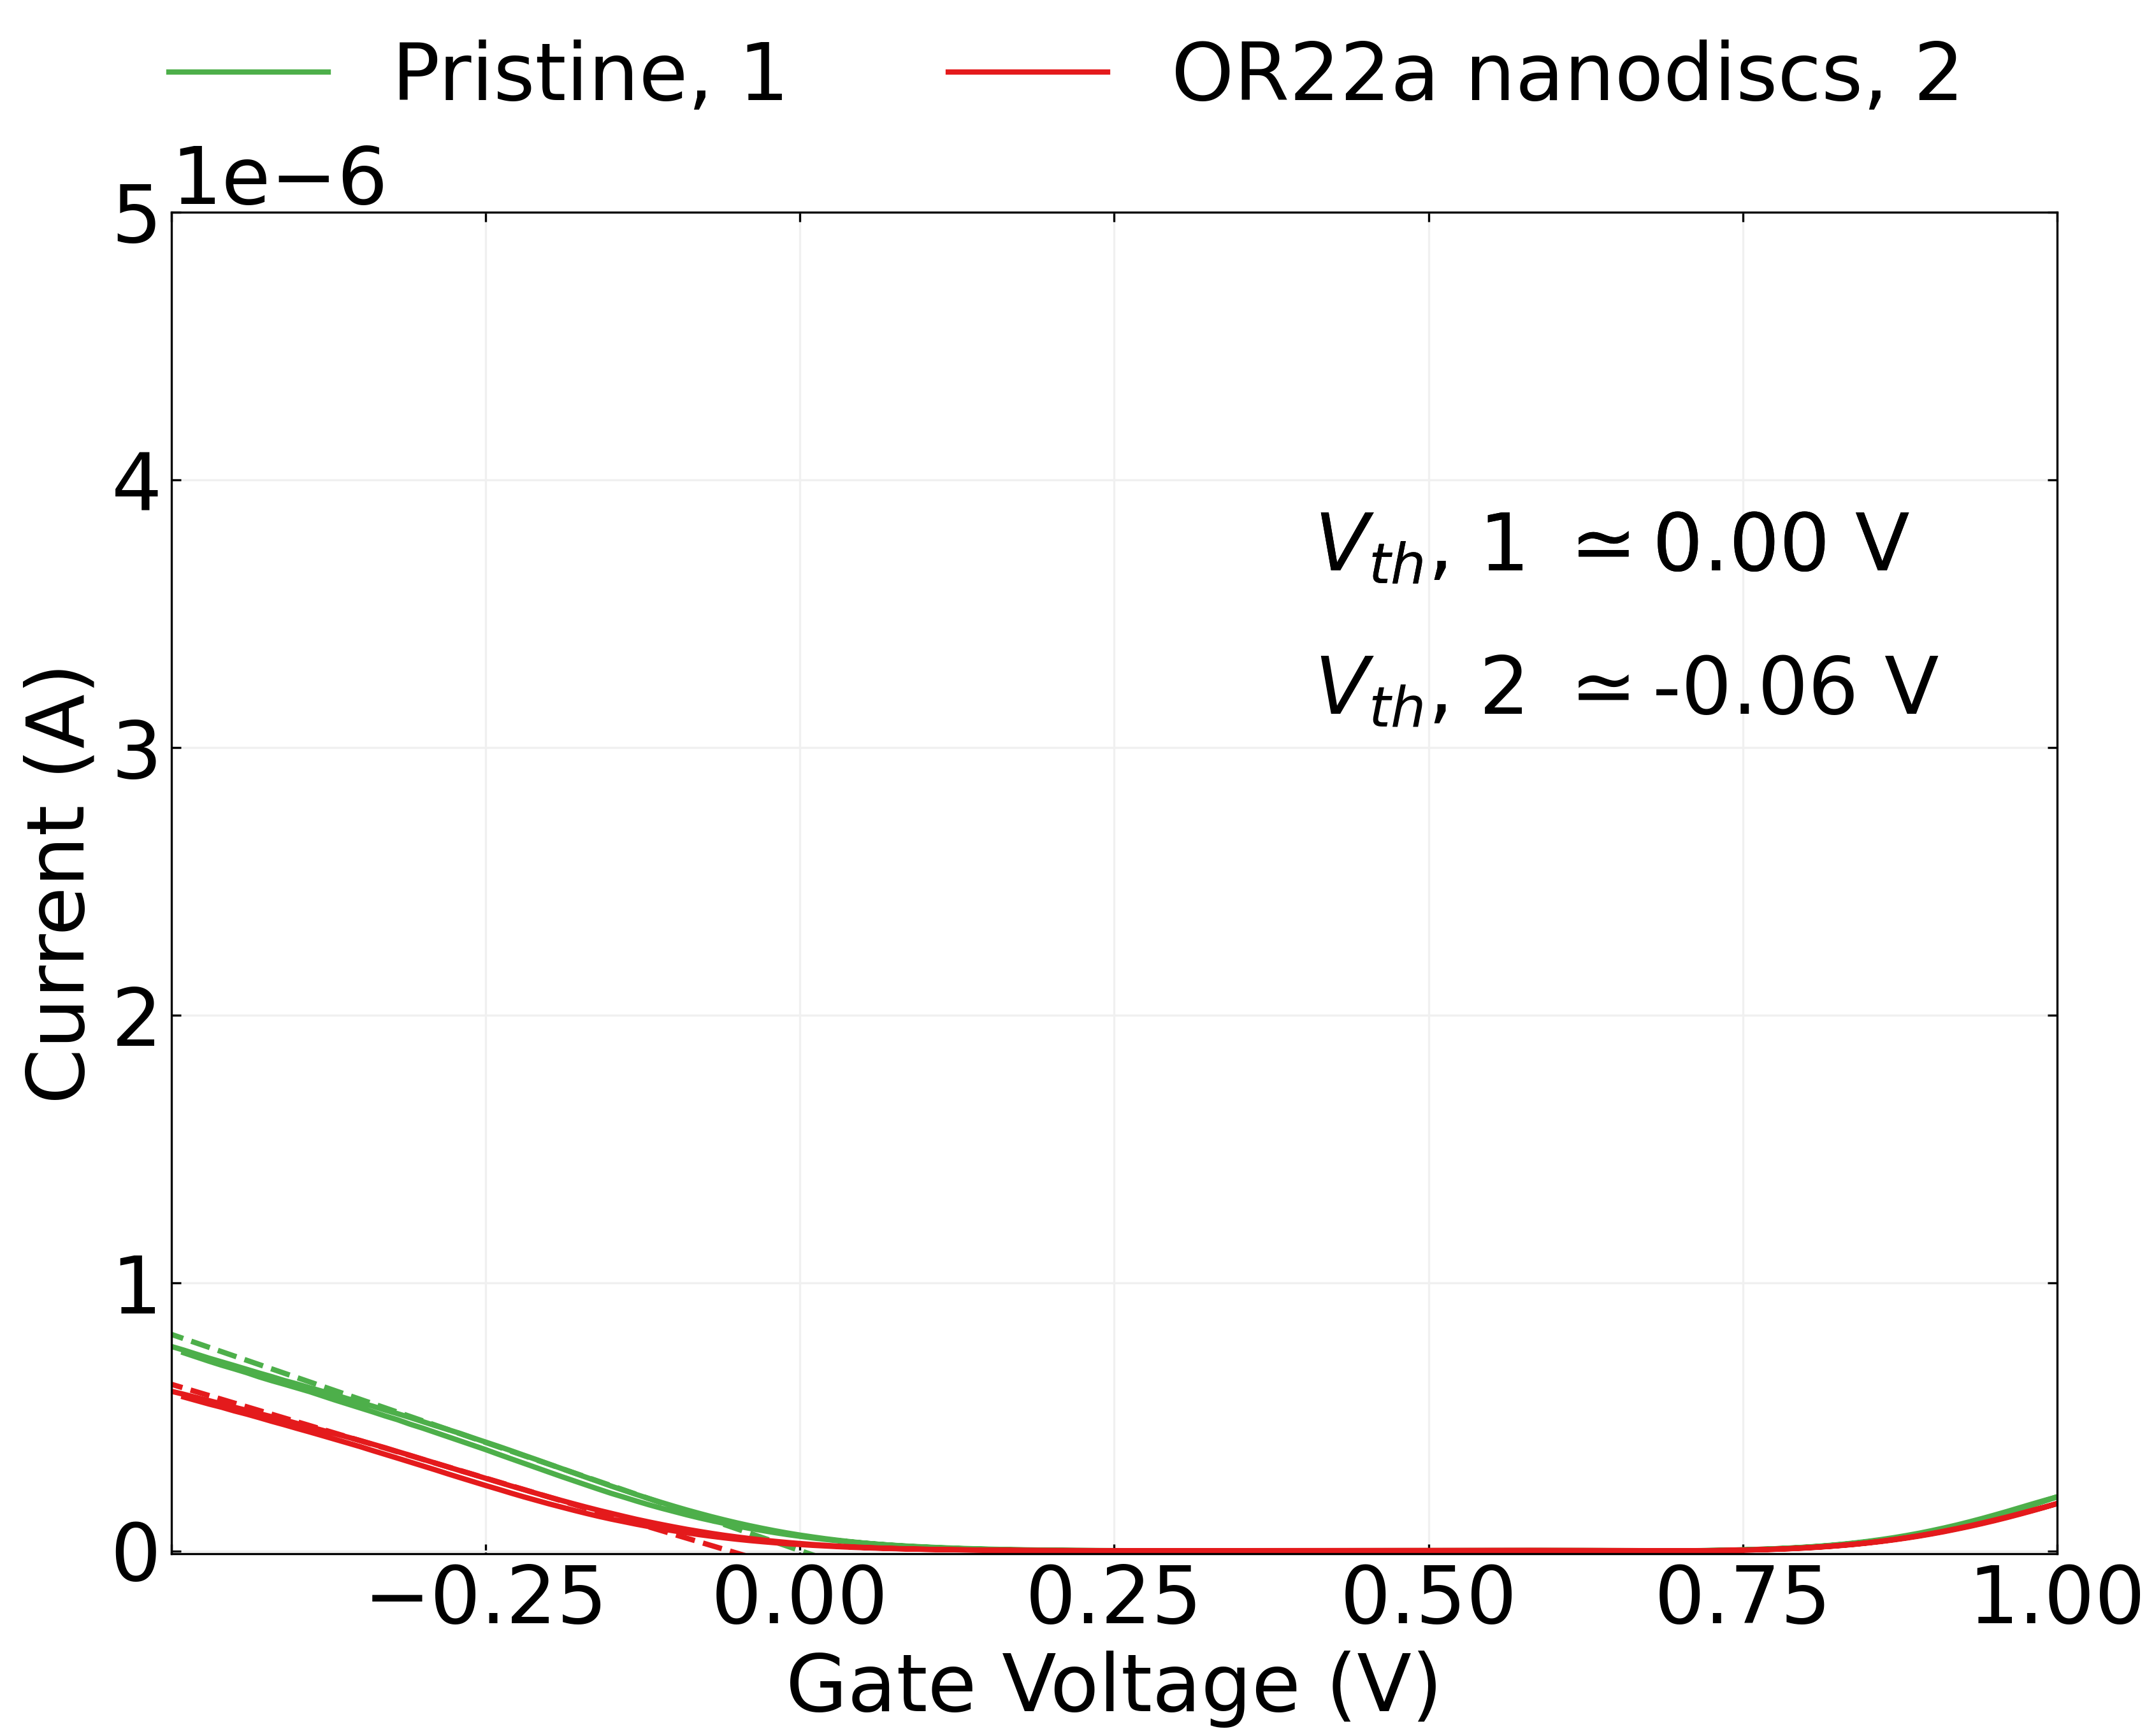
\includegraphics{figures/ch8/Q4C4_ch4.png}

}

}

\end{minipage}%
%
\begin{minipage}[t]{0.01\linewidth}

{\centering 

~

}

\end{minipage}%
%
\begin{minipage}[t]{0.03\linewidth}

{\centering 

\raisebox{-\height}{

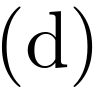
\includegraphics{figures/(d).png}

}

}

\end{minipage}%
%
\begin{minipage}[t]{0.01\linewidth}

{\centering 

~

}

\end{minipage}%
%
\begin{minipage}[t]{0.45\linewidth}

{\centering 

\raisebox{-\height}{

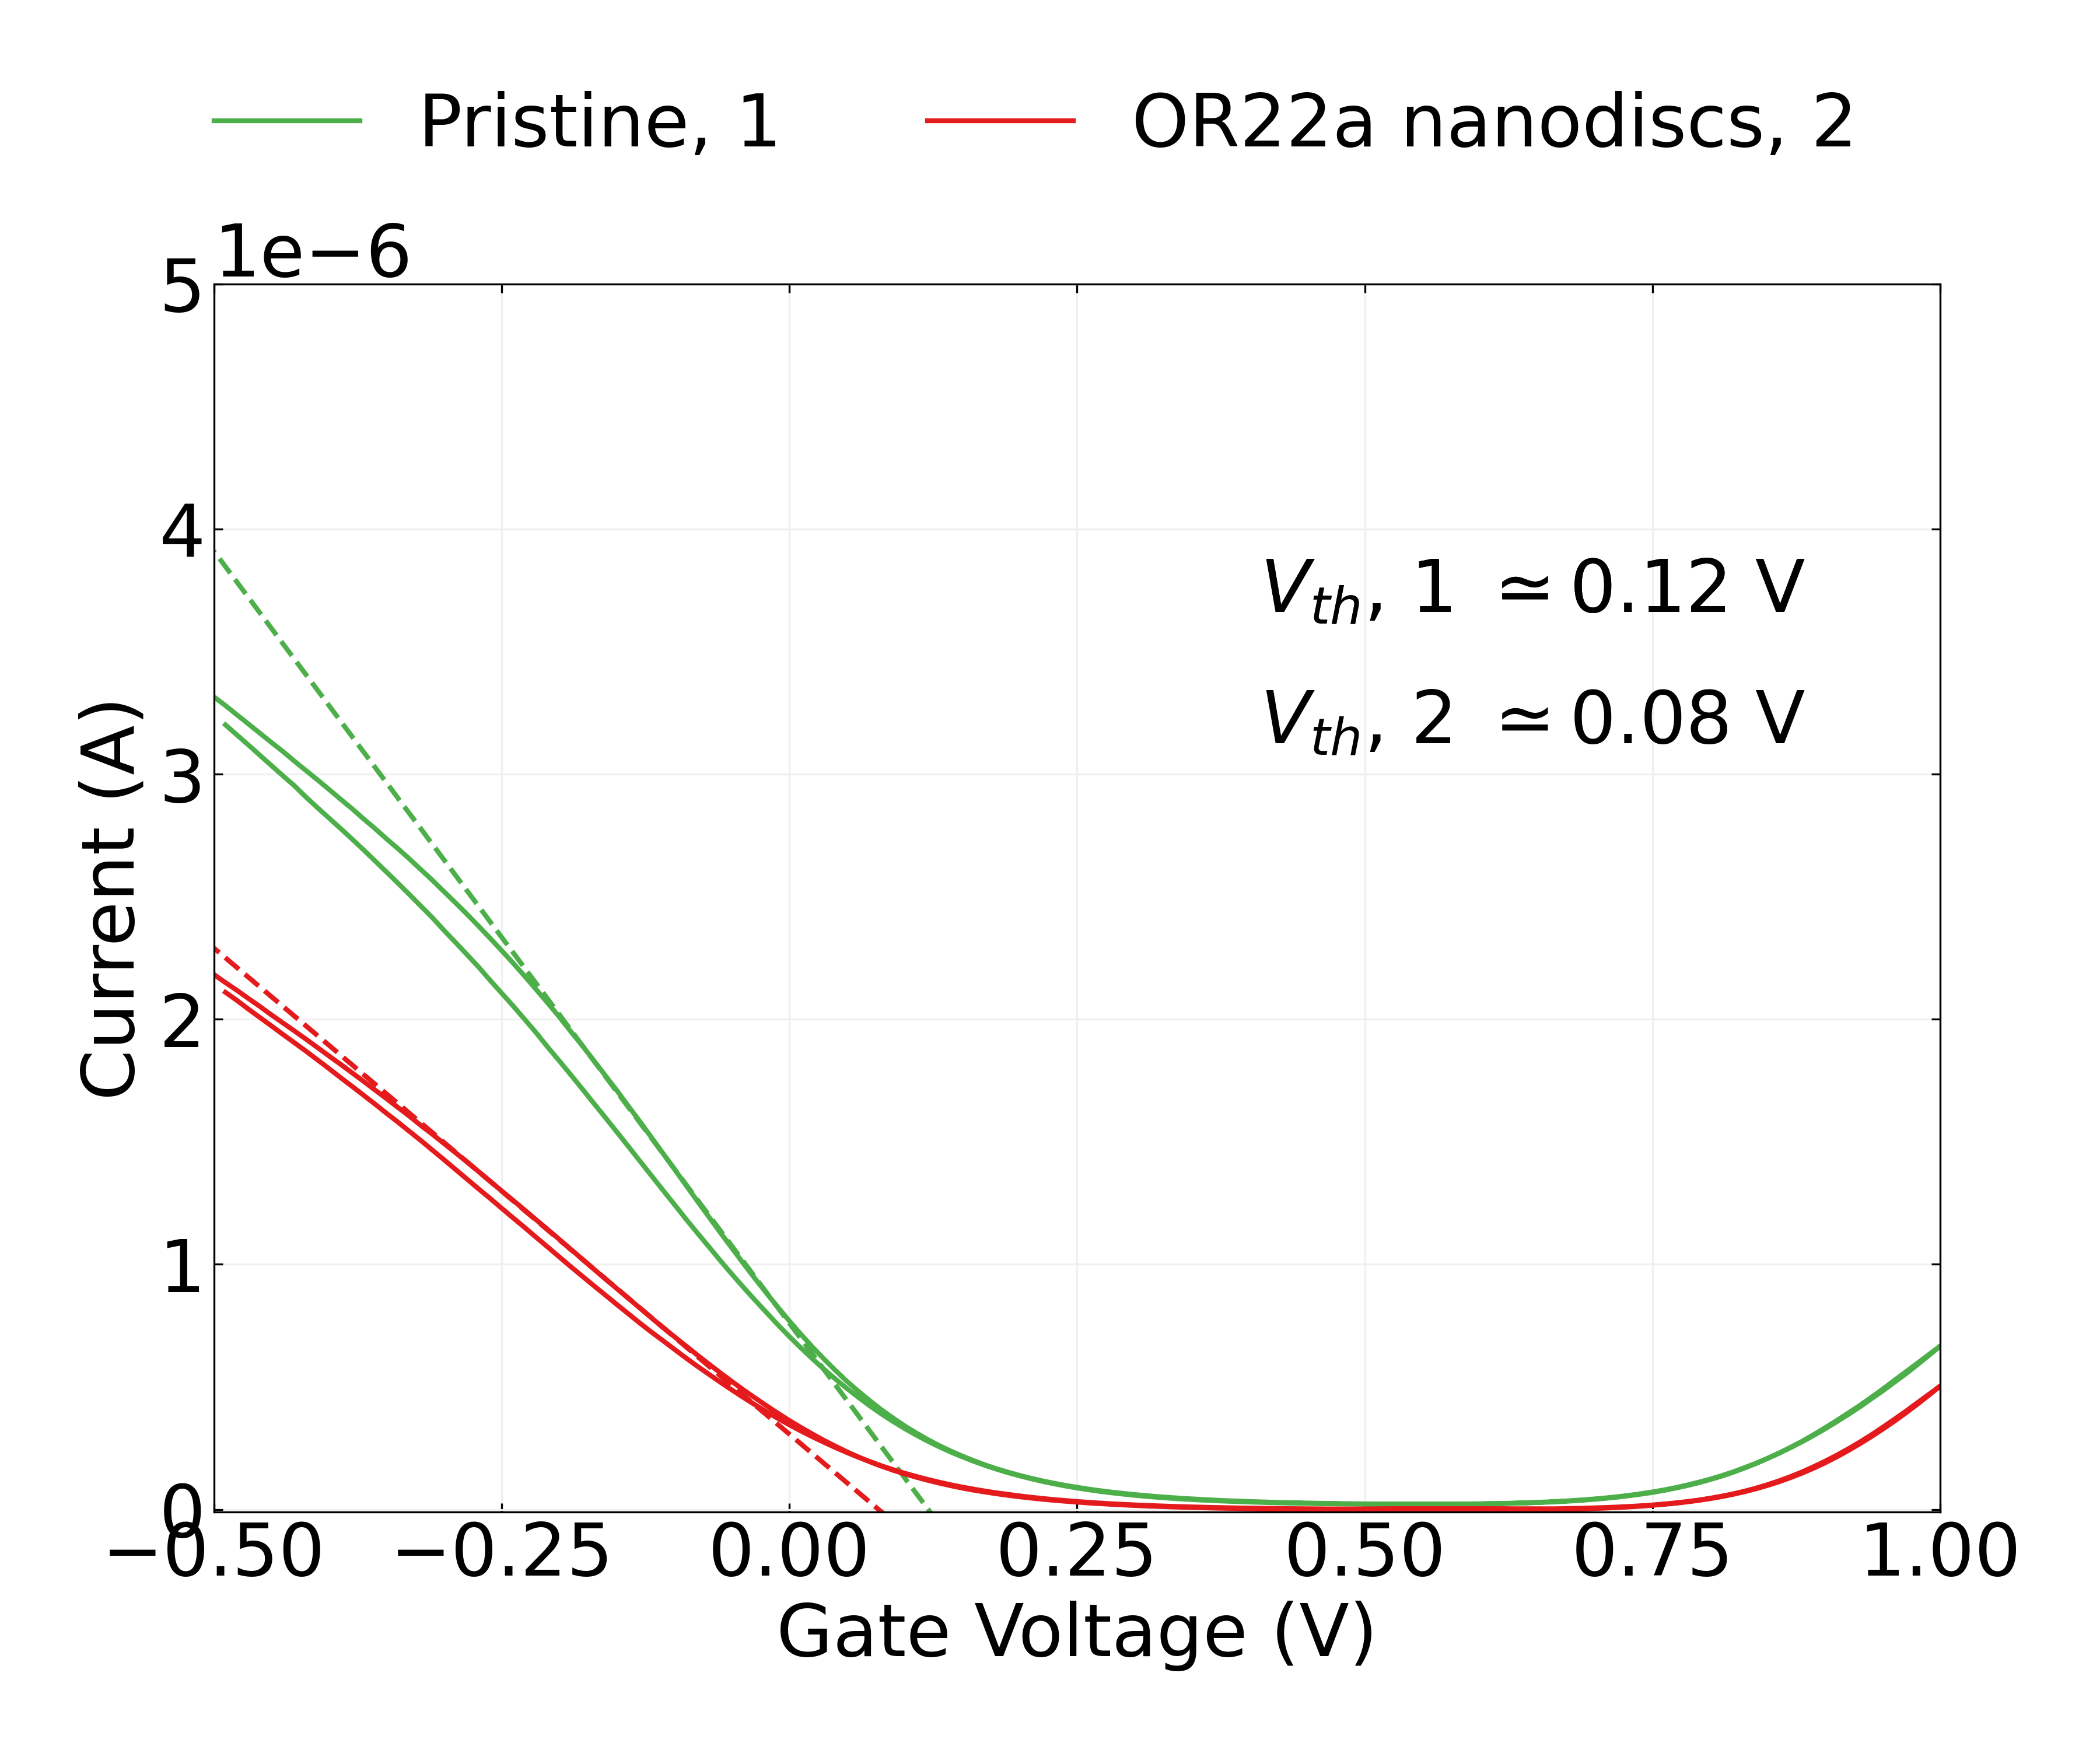
\includegraphics{figures/ch8/Q4C4_ch5.png}

}

}

\end{minipage}%
%
\begin{minipage}[t]{0.01\linewidth}

{\centering 

~

}

\end{minipage}%
\newline
\begin{minipage}[t]{0.03\linewidth}

{\centering 

\raisebox{-\height}{


\includegraphics{figures/(e).png}

}

}

\end{minipage}%
%
\begin{minipage}[t]{0.01\linewidth}

{\centering 

~

}

\end{minipage}%
%
\begin{minipage}[t]{0.45\linewidth}

{\centering 

\raisebox{-\height}{

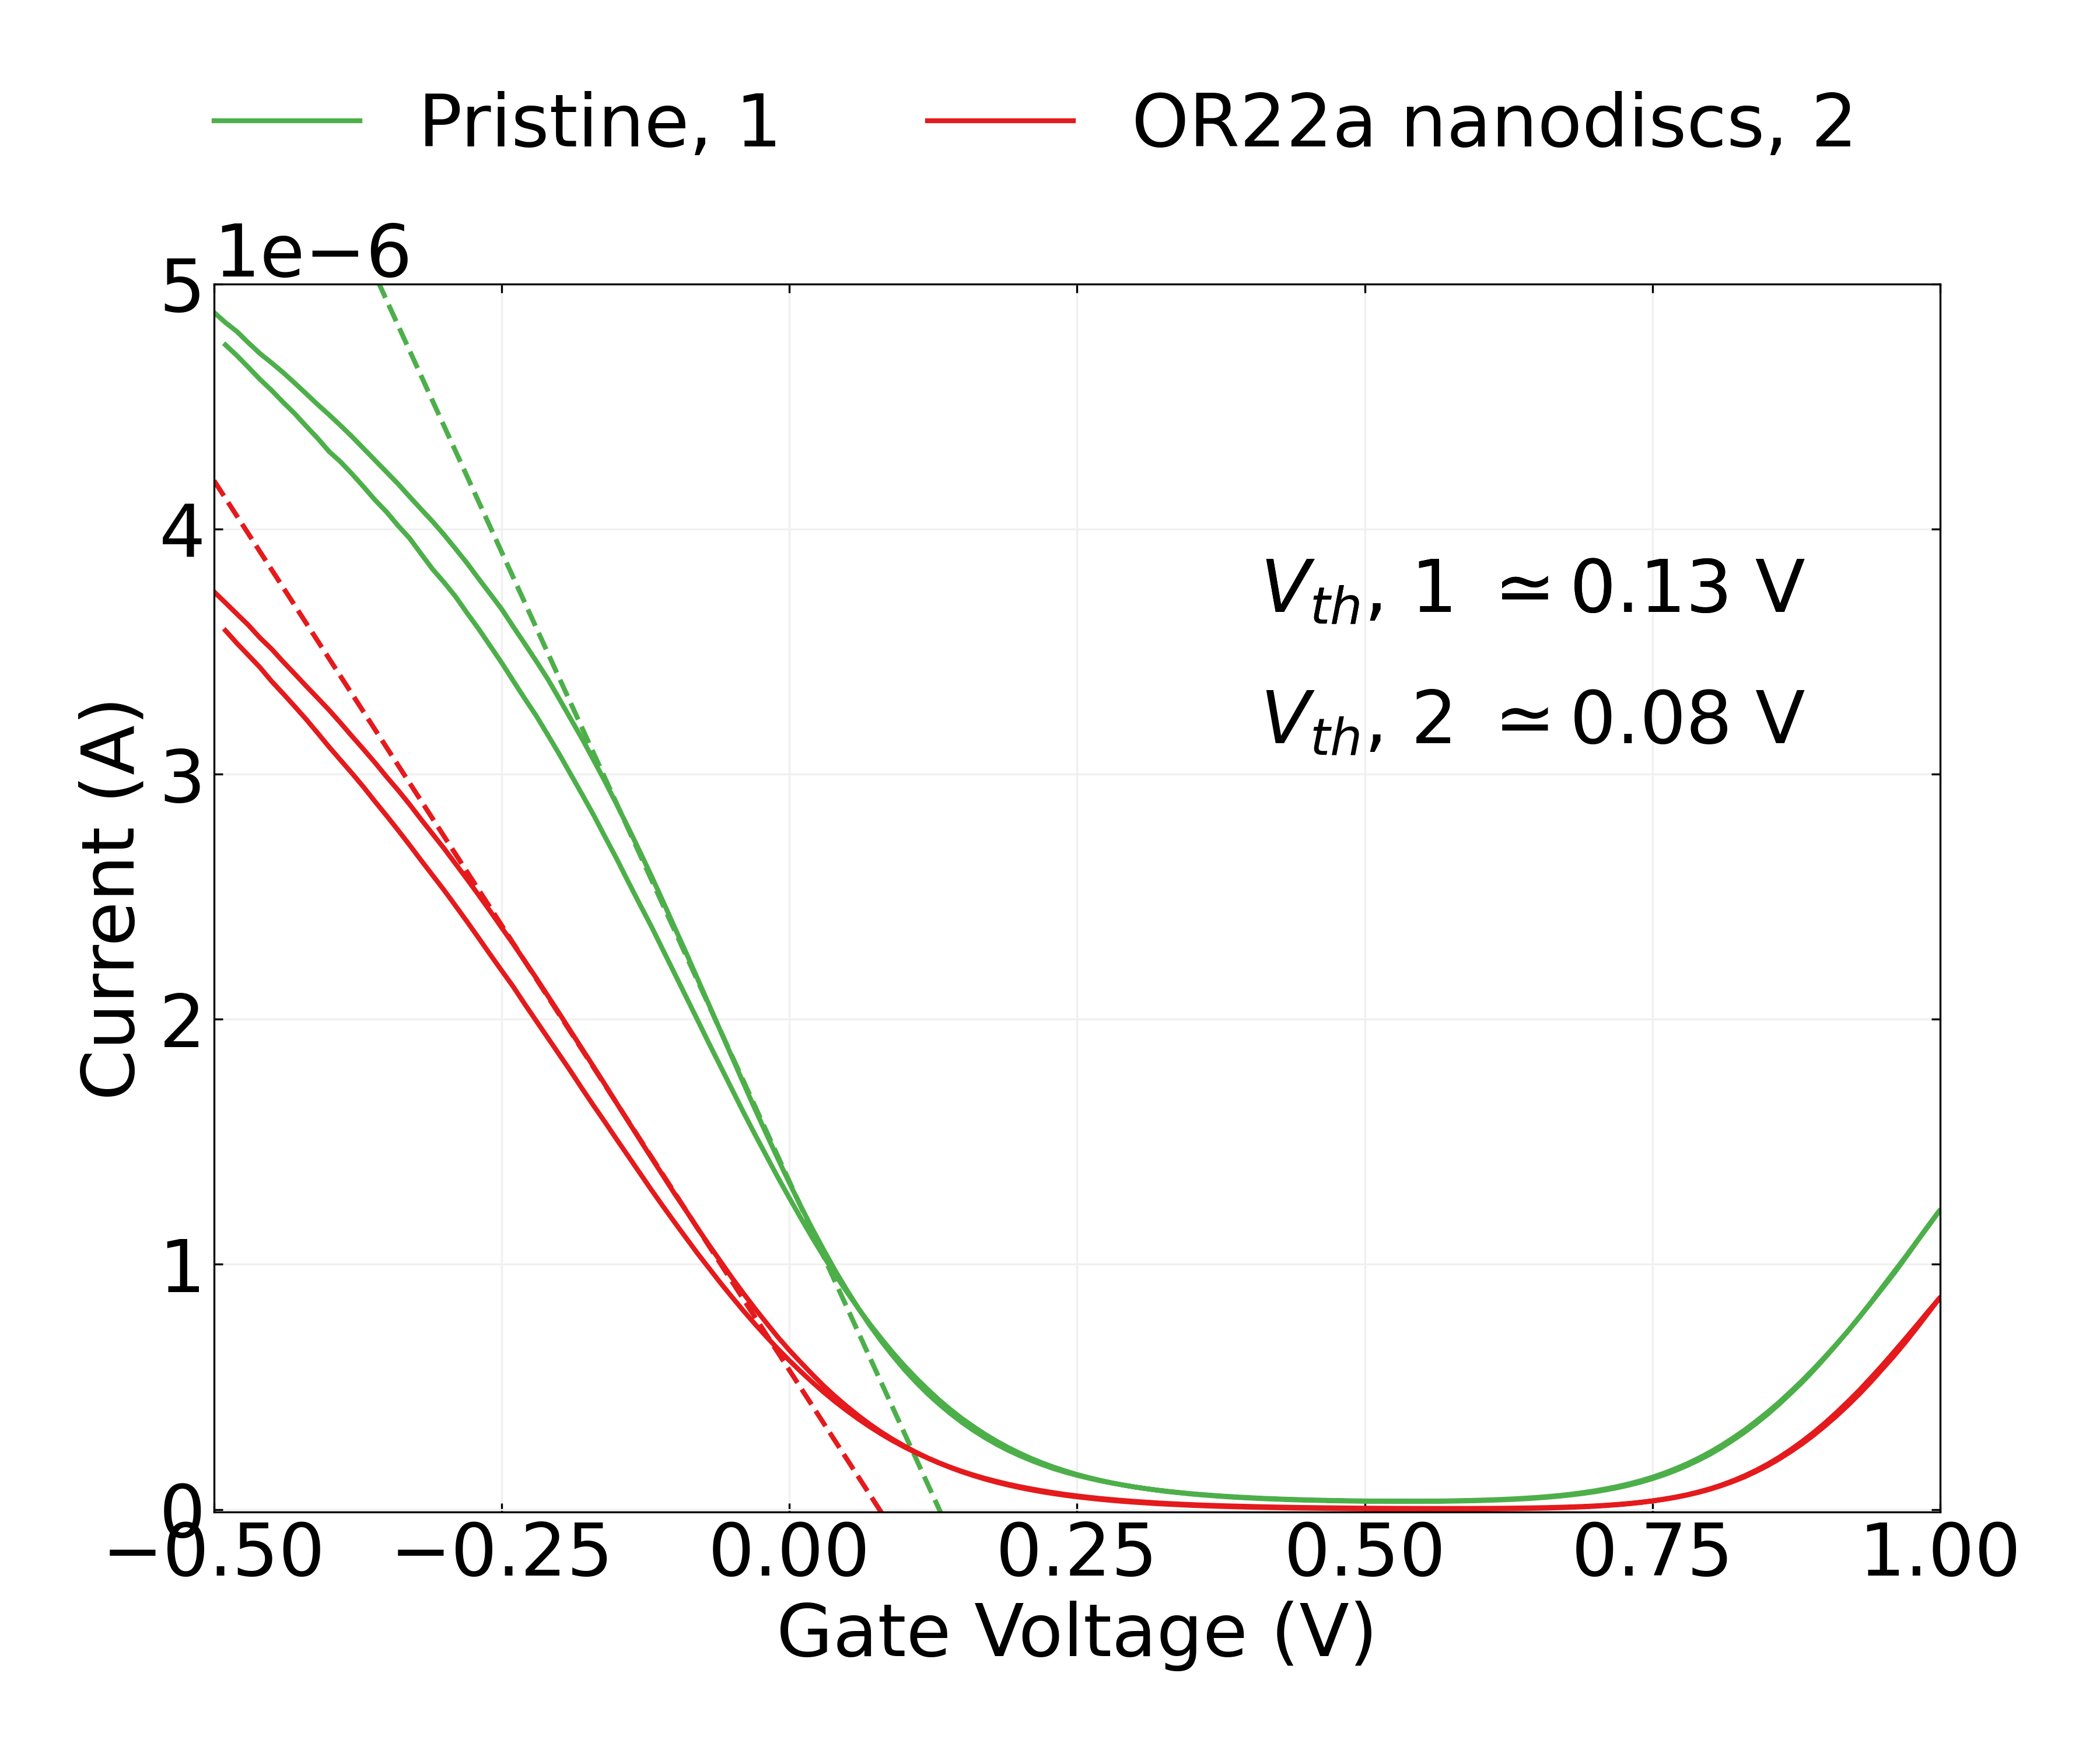
\includegraphics{figures/ch8/Q4C4_ch6.png}

}

}

\end{minipage}%
%
\begin{minipage}[t]{0.01\linewidth}

{\centering 

~

}

\end{minipage}%
%
\begin{minipage}[t]{0.03\linewidth}

{\centering 

\raisebox{-\height}{


\includegraphics{figures/(f).png}

}

}

\end{minipage}%
%
\begin{minipage}[t]{0.01\linewidth}

{\centering 

~

}

\end{minipage}%
%
\begin{minipage}[t]{0.45\linewidth}

{\centering 

\raisebox{-\height}{

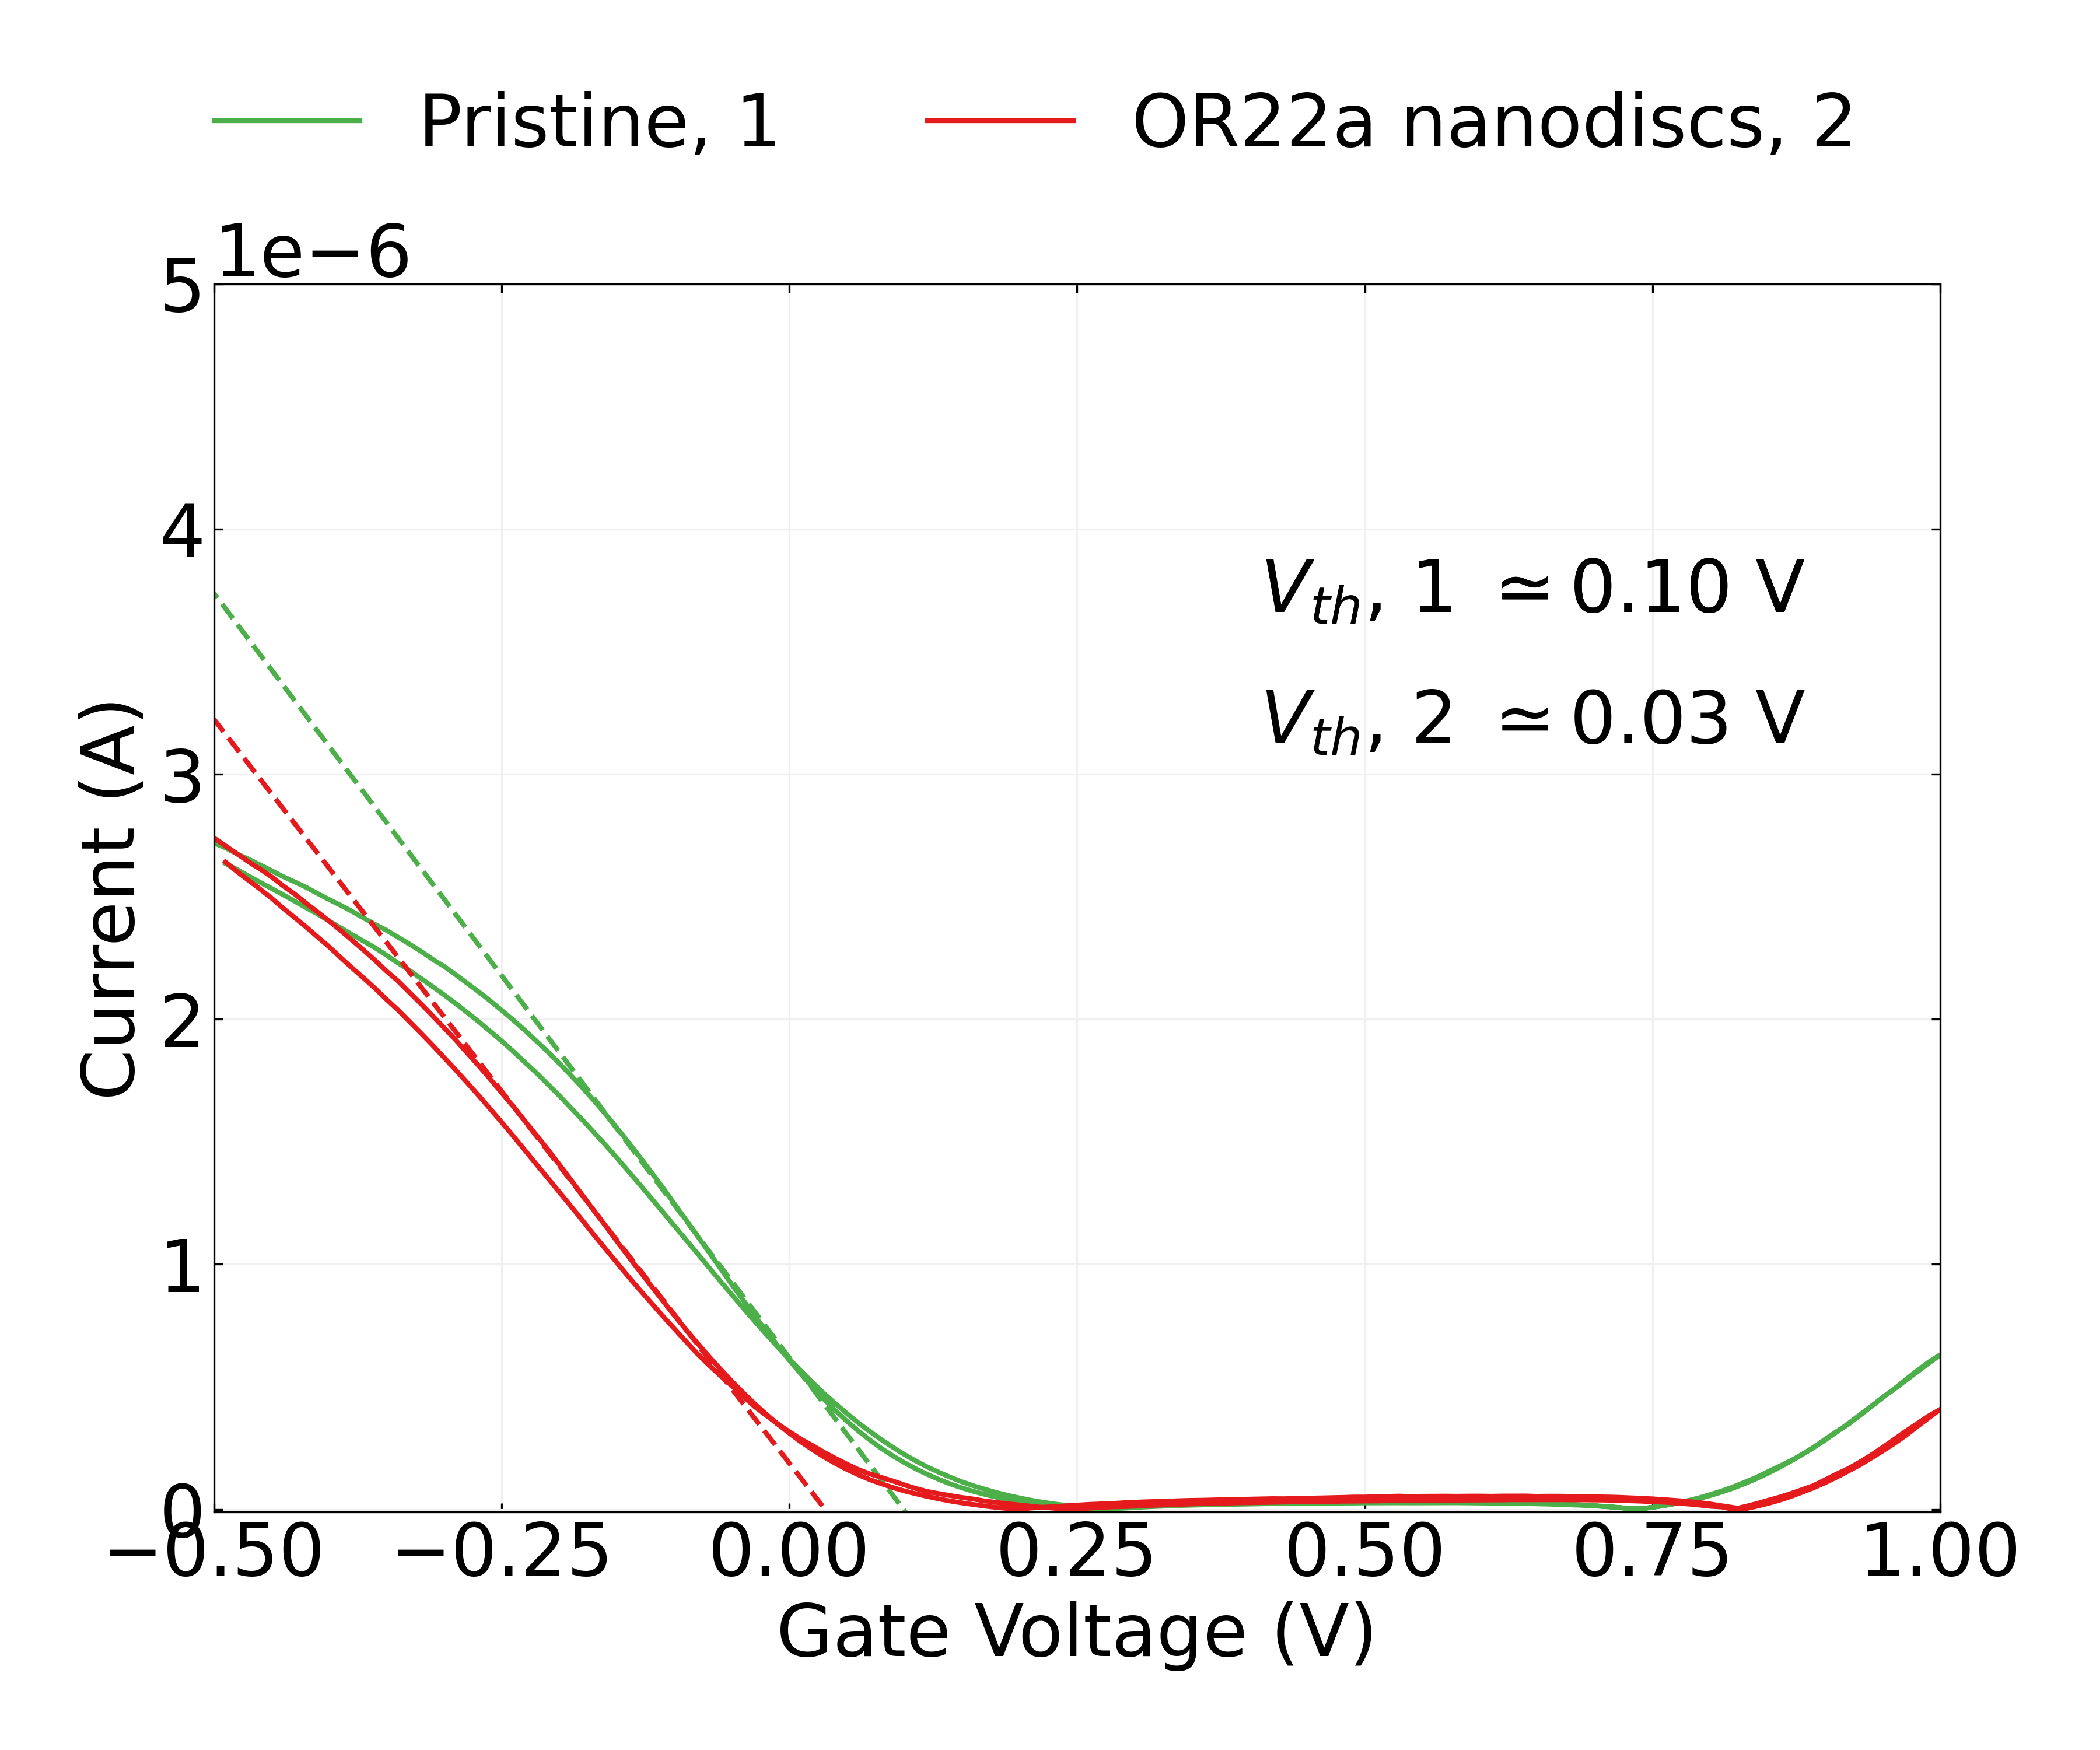
\includegraphics{figures/ch8/Q4C4_ch7.png}

}

}

\end{minipage}%
%
\begin{minipage}[t]{0.01\linewidth}

{\centering 

~

}

\end{minipage}%

\caption{\label{fig-OR22a-variability-TX}Liquid-gated carbon nanotube
network device transfer characteristics before and after OR22a nanodisc
functionalisation. Each subfigure (a)-(f) corresponds to a different
channel of the functionalised device; (a) corresponds to channel 2, (b)
corresponds to channel 3, (c) corresponds to channel 4, (d) corresponds
to channel 5, (e) corresponds to channel 6 and (f) corresponds to
channel 7. The dashed line shown is tangent to the subthreshold slope of
the characteristic curve. The threshold voltage corresponding to the
intercept of this slope with the x-axis is shown for each transfer
characteristic curve.}

\end{figure}

\begin{figure}

{\centering 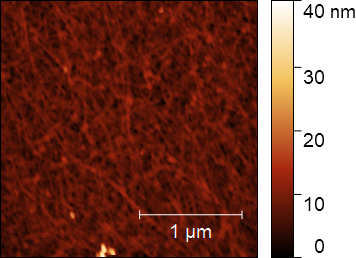
\includegraphics[width=0.5\textwidth,height=\textheight]{figures/ch8/Q4C4_CH6_PostSensing_OR22a_Func_AFM100670_00693.png}

}

\caption{\label{fig-OR22a-variability-AFM}An atomic force microscope
image of channel 6 from the OR22a nanodisc functionalised device which
showed no response to ethyl hexanoate.}

\end{figure}

\begin{figure}

\begin{minipage}[t]{0.03\linewidth}

{\centering 

\raisebox{-\height}{


\includegraphics{figures/(a).png}

}

}

\end{minipage}%
%
\begin{minipage}[t]{0.01\linewidth}

{\centering 

~

}

\end{minipage}%
%
\begin{minipage}[t]{0.45\linewidth}

{\centering 

\raisebox{-\height}{

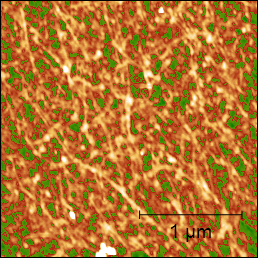
\includegraphics{figures/ch8/Q4C4_CH6_PostSensing_OR22a_Func_AFM100670_00693_mask.png}

}

}

\end{minipage}%
%
\begin{minipage}[t]{0.01\linewidth}

{\centering 

~

}

\end{minipage}%
%
\begin{minipage}[t]{0.03\linewidth}

{\centering 

\raisebox{-\height}{

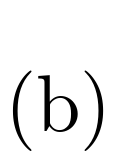
\includegraphics{figures/(b).png}

}

}

\end{minipage}%
%
\begin{minipage}[t]{0.01\linewidth}

{\centering 

~

}

\end{minipage}%
%
\begin{minipage}[t]{0.45\linewidth}

{\centering 

\raisebox{-\height}{

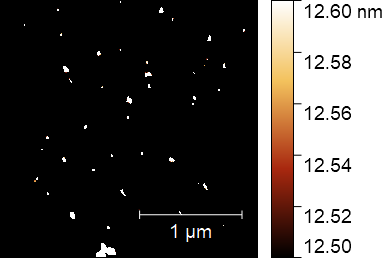
\includegraphics{figures/ch8/Q4C4_CH6_PostSensing_OR22a_Func_AFM100670_00693_12.5nm_crosssection.png}

}

}

\end{minipage}%
%
\begin{minipage}[t]{0.01\linewidth}

{\centering 

~

}

\end{minipage}%

\caption{\label{fig-OR22a-variability-AFM-comparison}The mask used to
find the average substrate height of the functionalised channel 6 is
shown in (a), with the substrate highlighted green. The bounds of the
colour map have been lowered in (a), as colour mapping over the full
height range makes it difficult to clearly distinguish between sub-20 nm
features and the substrate. A binary representation of the atomic force
microscope image with a threshold height of 12.5 nm is shown in (b).}

\end{figure}

Liquid-gated electrical characteristics were taken of each sensing
channel from this device before and after functionalisation with OR22a,
in the same manner as Section~\ref{sec-aqueous-sensing-EtHex}. These
characteristics are shown in Figure~\ref{fig-OR22a-variability-TX}. The
average threshold shift was \(-0.06\pm0.02\), the same as that of a
device functionalised with PBASE in methanol without subsequent
functionalisation with OR22a nanodiscs. To test whether protein was
present on the channel, an atomic force microscope image was taken of
channel 6, as shown in Figure~\ref{fig-OR22a-variability-AFM}. The same
image analysis as in Section~\ref{sec-aqueous-sensing-EtHex} was
performed, with the substrate mask shown in
Figure~\ref{fig-OR22a-variability-AFM-comparison} (a) giving an average
substrate height of \(3.8\pm0.4\). A binary representation of the image
with a 12.5 nm threshold, 8.7 nm above the average substrate height, is
shown in Figure~\ref{fig-OR22a-variability-AFM-comparison} (b). As with
the functionalised device in Figure~\ref{fig-crosssection} (b),
Figure~\ref{fig-OR22a-variability-AFM-comparison} (b) shows clustering
of features, many of which are larger than 50 nm across. It seems,
therefore, that nanodisc aggregates up to 27.5 nm high are present on
channel 6, despite the lack of a significant threshold shift as a result
of functionalisation.

\begin{figure}

{\centering 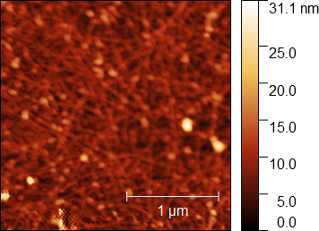
\includegraphics[width=0.5\textwidth,height=\textheight]{figures/ch8/00161_noPBASE.png}

}

\caption{\label{fig-OR22a-noPBASE-AFM}An atomic force microscope image
of a carbon nanotube film submerged in OR22a nanodiscs for 1 hour
without prior exposure to PBASE or methanol.}

\end{figure}

\begin{figure}

\begin{minipage}[t]{0.03\linewidth}

{\centering 

\raisebox{-\height}{


\includegraphics{figures/(a).png}

}

}

\end{minipage}%
%
\begin{minipage}[t]{0.01\linewidth}

{\centering 

~

}

\end{minipage}%
%
\begin{minipage}[t]{0.45\linewidth}

{\centering 

\raisebox{-\height}{

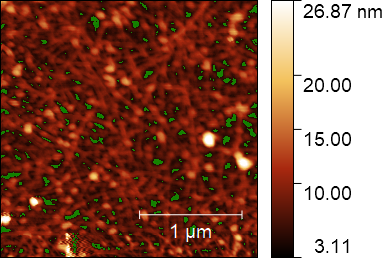
\includegraphics{figures/ch8/Ned_Q16D2_W4_OR22a1_noPBASE_sensing_2.5micron_256px_00462_20210921_mask.png}

}

}

\end{minipage}%
%
\begin{minipage}[t]{0.01\linewidth}

{\centering 

~

}

\end{minipage}%
%
\begin{minipage}[t]{0.03\linewidth}

{\centering 

\raisebox{-\height}{

\includegraphics{figures/(b).png}

}

}

\end{minipage}%
%
\begin{minipage}[t]{0.01\linewidth}

{\centering 

~

}

\end{minipage}%
%
\begin{minipage}[t]{0.45\linewidth}

{\centering 

\raisebox{-\height}{

\includegraphics{figures/ch8/Ned_Q16D2_W4_OR22a1_noPBASE_sensing_2.5micron_256px_00462_20210921_12.8nm_threshold.png}

}

}

\end{minipage}%
%
\begin{minipage}[t]{0.01\linewidth}

{\centering 

~

}

\end{minipage}%

\caption{\label{fig-OR22a-noPBASE-AFM-comparison}The binary
representation of the network, with a height threshold of 12.8 nm
(average substrate height = 4.1 nm), is shown in (b).}

\end{figure}

\begin{figure}

\begin{minipage}[t]{0.03\linewidth}

{\centering 

\raisebox{-\height}{

\includegraphics{figures/(a).png}

}

}

\end{minipage}%
%
\begin{minipage}[t]{0.01\linewidth}

{\centering 

~

}

\end{minipage}%
%
\begin{minipage}[t]{0.45\linewidth}

{\centering 

\raisebox{-\height}{

\includegraphics{figures/ch8/Q4C8_ch4_without_gate_current.png}

}

}

\end{minipage}%
%
\begin{minipage}[t]{0.03\linewidth}

{\centering 

~

}

\end{minipage}%
%
\begin{minipage}[t]{0.03\linewidth}

{\centering 

\raisebox{-\height}{

\includegraphics{figures/(b).png}

}

}

\end{minipage}%
%
\begin{minipage}[t]{0.45\linewidth}

{\centering 

\raisebox{-\height}{

\includegraphics{figures/ch8/Q4C8_filtered_detrend_trunc_arrows_normalised.png}

}

}

\end{minipage}%

\caption{\label{fig-OR22a-variability-TX-comparison}The device
characteristics in (a) are from channel 4 of the device placed in OR22a
nanodisc solution for 1 hour without prior exposure to PBASE or methanol
before and after functionalisation. Real-time sampling using this
channel is shown in (b). A 20 µL addition of 1\% DMSO 1XPBS was made at
200 s. Subsequently, 20 µL additions of ethyl hexanoate diluted in 1\%
DMSO 1XPBS were made at 400 s, 600 s, 800 s and 1000 s and 1200 s, with
the concentration of each addition indicated above the time of
addition.}

\end{figure}

Both OR nanodisc and empty nanodisc attachment via PBASE have been shown
to cause significant gating of the network
(Section~\ref{sec-aqueous-sensing-EtHex}). Therefore, it might be
reasoned that the lack of a gating effect, but with nanodiscs present,
results from a direct attachment mechanism circumventing the PBASE
linker. The amine group on proteins can be attached directly onto carbon
nanotubes by adsorption, although this attachment is relatively weak
\autocite{Bradley2004}. Figure~\ref{fig-OR22a-noPBASE-AFM} shows an AFM
image of a carbon nanotube network film after submersion in a 10 μL/mL
OR22a nanodisc in PBS solution for 1 hour (batch NDOR22a-0016-1),
without prior exposure to PBASE in methanol.
Figure~\ref{fig-OR22a-noPBASE-AFM-comparison} shows the substrate mask
in (a) and a binary representation of this AFM with nanodisc aggregates
clearly visible in (b). In
Figure~\ref{fig-OR22a-variability-TX-comparison} (a), the negative
threshold shift of a channel modified in this way was -0.27 V, similar
in size to the shift due to functionalisation seen for the working
biosensor. However, this device channel did not work as a sensor when
tested with ethyl hexanoate.
Figure~\ref{fig-OR22a-variability-TX-comparison} (b) shows a small,
positive current response to additions of ethyl hexanoate diluted in 1\%
DMSO 1XPBS, which may result from the weakly attached OR22a nanodiscs
being mechanically removed by the pressure of each addition on the
device channels.

An explanation is required for the seemingly contradictory situation
where nanodiscs can be present on a device channel without significant
gating effects. The most straightforward explanation is that no reliable
correlation exist between the two phenomena. Given the consistent
threshold shift results for various linker functionalisations seen in
\textbf{?@sec-noncovalent-functionalisation}, this scenario implies a
significant variation in protein structure and charge behaviour within a
single nanodisc batch, which seems unlikely. Another possibility is that
some type of surface coating is causing nanodiscs to not attach to
either PBASE or the carbon nanotubes. This surface coating might be
attractive, attaching to both nanodiscs and carbon nanotubes, but
forming a barrier layer between the two. Alternatively, this coating
might be repulsive, causing nanodiscs to attach weakly to the substrate
around the carbon nanotubes. Variations in the degree to which a network
is coated may then explain why the same functionalisation method might
work for one device but not another. The following section investigates
ways of eliminating possible sources of surface coating for more
reliable functionalisation results.

\hypertarget{sec-contamination}{%
\subsection{Potential Sources of Variability}\label{sec-contamination}}

Throughout the course of this thesis, multiple potential candidates for
the unwanted surface coating discussed in the previous section have been
identified. These include the surfactant used in carbon nanotube
deposition (\textbf{?@sec-pristine-morphology},
\textbf{?@sec-pristine-electrical-characterisation}) and the solvent
used in functionalisation
(\textbf{?@sec-PBASE-electrical-characterisation}). Another possibility
is that PBASE itself is acting as a surface coating, which could result
from multilayer coverage restricting access to directly attached PBASE
(\textbf{?@sec-PBASE-attachment}). Alternatively, PBASE may have
hydrolysed into PBA prior to attachment, forming an inert surface layer
upon \(\pi\)-stacking around the carbon nanotubes. However, no threshold
shift directly attributable to PBA attachment should occur
(\textbf{?@sec-PBA-characterisation}), and this is not what was observed
when characterising the non-working device in
Section~\ref{sec-variability}. To understand which of these candidates
is responsible for the significant variability in biosensor
functionality, the sensing procedure was performed with slight
variations on the biosensor fabrication and functionalisation
procedures. In each test, an individual element of one of these
procedures was altered to prevent the introduction of a specific surface
coating. The biosensor was then characterised and tested to see if it
would respond to its target odorant.

\hypertarget{surfactant-contamination}{%
\subsubsection*{Surfactant
Contamination}\label{surfactant-contamination}}
\addcontentsline{toc}{subsubsection}{Surfactant Contamination}

Two different approaches were trialled to eliminate possible surfactant
contamination, both of which drew heavily on previous methods used for
iOR biosensor fabrication \autocite{Murugathas2019b,Murugathas2020}.
Solvent-deposited carbon nanotube network and graphene devices were
fabricated as described in \textbf{?@sec-qw-processing}. The same
functionalisation process for each device was used as described in
Section~\ref{sec-working-PBASE-functionalisation} with OR22a nanodiscs.

\begin{figure}

\begin{minipage}[t]{0.11\linewidth}

{\centering 

~

}

\end{minipage}%
%
\begin{minipage}[t]{0.03\linewidth}

{\centering 

\raisebox{-\height}{

\includegraphics{figures/(a).png}

}

}

\end{minipage}%
%
\begin{minipage}[t]{0.01\linewidth}

{\centering 

~

}

\end{minipage}%
%
\begin{minipage}[t]{0.70\linewidth}

{\centering 

\raisebox{-\height}{

\includegraphics{figures/ch8/NTQ25C5_OR22a_sample_220126_detrend_trunc_arrows_normalised.png}

}

}

\end{minipage}%
%
\begin{minipage}[t]{0.15\linewidth}

{\centering 

~

}

\end{minipage}%
\newline
\begin{minipage}[t]{0.11\linewidth}

{\centering 

~

}

\end{minipage}%
%
\begin{minipage}[t]{0.03\linewidth}

{\centering 

\raisebox{-\height}{

\includegraphics{figures/(b).png}

}

}

\end{minipage}%
%
\begin{minipage}[t]{0.01\linewidth}

{\centering 

~

}

\end{minipage}%
%
\begin{minipage}[t]{0.70\linewidth}

{\centering 

\raisebox{-\height}{

\includegraphics{figures/ch8/NTQ25C5_OR22a_sample_220126_filtered_detrend_trunc_arrows_normalised.png}

}

}

\end{minipage}%
%
\begin{minipage}[t]{0.15\linewidth}

{\centering 

~

}

\end{minipage}%

\caption{\label{fig-solvent-deposited-sensing}The normalised sensing
series of the solvent-deposited, OR22a-functionalised device across six
multiplexed channels, where current data has been despiked and baseline
drift removed. The concentration of each 20 µL addition is indicated
above the time of addition. The same sensing series is shown in both (a)
and (b), where a moving median filter has been applied in (b).}

\end{figure}

\begin{figure}

\begin{minipage}[t]{0.03\linewidth}

{\centering 

\raisebox{-\height}{

\includegraphics{figures/(a).png}

}

}

\end{minipage}%
%
\begin{minipage}[t]{0.01\linewidth}

{\centering 

~

}

\end{minipage}%
%
\begin{minipage}[t]{0.45\linewidth}

{\centering 

\raisebox{-\height}{

\includegraphics{figures/ch8/NTQ25C5_ch1.png}

}

}

\end{minipage}%
%
\begin{minipage}[t]{0.01\linewidth}

{\centering 

~

}

\end{minipage}%
%
\begin{minipage}[t]{0.03\linewidth}

{\centering 

\raisebox{-\height}{

\includegraphics{figures/(b).png}

}

}

\end{minipage}%
%
\begin{minipage}[t]{0.01\linewidth}

{\centering 

~

}

\end{minipage}%
%
\begin{minipage}[t]{0.45\linewidth}

{\centering 

\raisebox{-\height}{

\includegraphics{figures/ch8/NTQ25C5_ch2.png}

}

}

\end{minipage}%
%
\begin{minipage}[t]{0.01\linewidth}

{\centering 

~

}

\end{minipage}%
\newline
\begin{minipage}[t]{0.03\linewidth}

{\centering 

\raisebox{-\height}{

\includegraphics{figures/(c).png}

}

}

\end{minipage}%
%
\begin{minipage}[t]{0.01\linewidth}

{\centering 

~

}

\end{minipage}%
%
\begin{minipage}[t]{0.45\linewidth}

{\centering 

\raisebox{-\height}{

\includegraphics{figures/ch8/NTQ25C5_ch3.png}

}

}

\end{minipage}%
%
\begin{minipage}[t]{0.01\linewidth}

{\centering 

~

}

\end{minipage}%
%
\begin{minipage}[t]{0.03\linewidth}

{\centering 

\raisebox{-\height}{

\includegraphics{figures/(d).png}

}

}

\end{minipage}%
%
\begin{minipage}[t]{0.01\linewidth}

{\centering 

~

}

\end{minipage}%
%
\begin{minipage}[t]{0.45\linewidth}

{\centering 

\raisebox{-\height}{

\includegraphics{figures/ch8/NTQ25C5_ch4.png}

}

}

\end{minipage}%
%
\begin{minipage}[t]{0.01\linewidth}

{\centering 

~

}

\end{minipage}%
\newline
\begin{minipage}[t]{0.03\linewidth}

{\centering 

\raisebox{-\height}{

\includegraphics{figures/(e).png}

}

}

\end{minipage}%
%
\begin{minipage}[t]{0.01\linewidth}

{\centering 

~

}

\end{minipage}%
%
\begin{minipage}[t]{0.45\linewidth}

{\centering 

\raisebox{-\height}{

\includegraphics{figures/ch8/NTQ25C5_ch5.png}

}

}

\end{minipage}%
%
\begin{minipage}[t]{0.01\linewidth}

{\centering 

~

}

\end{minipage}%
%
\begin{minipage}[t]{0.03\linewidth}

{\centering 

\raisebox{-\height}{

\includegraphics{figures/(f).png}

}

}

\end{minipage}%
%
\begin{minipage}[t]{0.01\linewidth}

{\centering 

~

}

\end{minipage}%
%
\begin{minipage}[t]{0.45\linewidth}

{\centering 

\raisebox{-\height}{

\includegraphics{figures/ch8/NTQ25C5_ch6.png}

}

}

\end{minipage}%
%
\begin{minipage}[t]{0.01\linewidth}

{\centering 

~

}

\end{minipage}%

\caption{\label{fig-solvent-deposited-sensing-TX}Liquid-gated
solvent-deposited carbon nanotube device transfer characteristics before
and after OR22a nanodisc functionalisation. (a) corresponds to channel
2, (b) corresponds to channel 3, (c) corresponds to channel 4, (d)
corresponds to channel 5, (e) corresponds to channel 6 and (f)
corresponds to channel 7. The dashed line shown is tangent to the
subthreshold slope of the characteristic curve. The threshold voltage
corresponding to the intercept of this slope with the x-axis is shown
for each transfer characteristic curve.}

\end{figure}

\begin{figure}

\begin{minipage}[t]{0.03\linewidth}

{\centering 

\raisebox{-\height}{

\includegraphics{figures/(a).png}

}

}

\end{minipage}%
%
\begin{minipage}[t]{0.01\linewidth}

{\centering 

~

}

\end{minipage}%
%
\begin{minipage}[t]{0.46\linewidth}

{\centering 

\raisebox{-\height}{

\includegraphics{figures/ch8/Ned_NTQ25C5_W4_20220126_00245_mask.png}

}

}

\end{minipage}%
%
\begin{minipage}[t]{0.03\linewidth}

{\centering 

\raisebox{-\height}{

\includegraphics{figures/(b).png}

}

}

\end{minipage}%
%
\begin{minipage}[t]{0.01\linewidth}

{\centering 

~

}

\end{minipage}%
%
\begin{minipage}[t]{0.46\linewidth}

{\centering 

\raisebox{-\height}{

\includegraphics{figures/ch8/Ned_NTQ25C5_W4_20220126_00245_section.png}

}

}

\end{minipage}%
%
\begin{minipage}[t]{0.01\linewidth}

{\centering 

~

}

\end{minipage}%
\newline
\begin{minipage}[t]{0.03\linewidth}

{\centering 

\raisebox{-\height}{

\includegraphics{figures/(c).png}

}

}

\end{minipage}%
%
\begin{minipage}[t]{0.01\linewidth}

{\centering 

~

}

\end{minipage}%
%
\begin{minipage}[t]{0.45\linewidth}

{\centering 

\raisebox{-\height}{

\includegraphics{figures/ch8/Ned_NTQ13_D11_dep50min_OR22a_dep1hr_20210211_00089.png}

}

}

\end{minipage}%
%
\begin{minipage}[t]{0.01\linewidth}

{\centering 

~

}

\end{minipage}%
%
\begin{minipage}[t]{0.03\linewidth}

{\centering 

\raisebox{-\height}{

\includegraphics{figures/(d).png}

}

}

\end{minipage}%
%
\begin{minipage}[t]{0.01\linewidth}

{\centering 

~

}

\end{minipage}%
%
\begin{minipage}[t]{0.45\linewidth}

{\centering 

\raisebox{-\height}{

\includegraphics{figures/ch8/Ned_NTQ13_D11_dep50min_OR22a_dep1hr_20210211_00088.png}

}

}

\end{minipage}%
%
\begin{minipage}[t]{0.01\linewidth}

{\centering 

~

}

\end{minipage}%

\caption{\label{fig-solvent-deposited-AFM-comparison}An 2.5 µm
\(\times\) 2.5 µm atomic force microscope image of an OR22a nanodisc
functionalised solvent-deposited carbon nanotube film is shown in (a),
with the average substrate height highlighted green. A binary
representation of the atomic force microscope image with a threshold
height of 34.7 nm is shown in (b). 10 µm \(\times\) 10 µm and 50 µm
\(\times\) 50 µm atomic force microscope images of another film
functionalised in the same manner are shown in (c) and (d)
respectively.}

\end{figure}

The normalised sensing behaviour for the solvent-deposited carbon
nanotube device is shown in Figure~\ref{fig-solvent-deposited-sensing}.
The device is largely unresponsive at each addition, with a slight
current increase on four channels with the 10 fM ethyl hexanoate
addition, and a slight decrease on five channels with the 100 fM EtHex
addition. No current change exceeded 2\%, and as shown in
Figure~\ref{fig-solvent-deposited-sensing} (b), the current changes
appear negligible on the scale of the changes seen in
Section~\ref{sec-EtHex-aqueous-sensing}. The average threshold shift
from functionalisation was \(-0.02\pm0.01\) V, which indicates
attachment of PBASE but not nanodiscs. As the device was made using the
pre-2023 encapsulation mask, an AFM was taken of a separate film
modified in the same manner, shown in
Figure~\ref{fig-solvent-deposited-AFM-comparison} (a). The average
substrate height was \(11.3\pm0.9\) nm. A binary representation of the
image taken at the minimum height no spindle-like bundles were visible,
46.1 nm, is shown in Figure~\ref{fig-solvent-deposited-AFM-comparison}
(b). Attached nanodisc aggregations are clearly visible, and appear
closer in nature to those observed for an OR35a-functionalised film
\autocite{Murugathas2020} than previously seen in this work.
Figure~\ref{fig-solvent-deposited-AFM-comparison} (c) and (d) show that
over a larger scale these aggregations can be at least 330 nm tall,
forming large clusters which may indicate mutual interaction during
deposition.

\begin{figure}

{\centering \includegraphics[width=0.7\textwidth,height=\textheight]{figures/ch8/Q3C3_filtered_trunc_arrows_normalised.png}

}

\caption{\label{fig-graphene-sensing}A normalised ethyl hexanoate
sensing series taken with a OR22a-functionalised graphene device. The
concentration of each 20 µL addition is indicated above the time of
addition, with additions made at 500 s, 1000 s, 1500 s, 2000 s and 2500
s.}

\end{figure}

\begin{figure}

\begin{minipage}[t]{0.03\linewidth}

{\centering 

\raisebox{-\height}{

\includegraphics{figures/(a).png}

}

}

\end{minipage}%
%
\begin{minipage}[t]{0.01\linewidth}

{\centering 

~

}

\end{minipage}%
%
\begin{minipage}[t]{0.45\linewidth}

{\centering 

\raisebox{-\height}{

\includegraphics{figures/ch8/Q3C3_ch6_PBASE_OR22a.png}

}

}

\end{minipage}%
%
\begin{minipage}[t]{0.01\linewidth}

{\centering 

~

}

\end{minipage}%
%
\begin{minipage}[t]{0.03\linewidth}

{\centering 

\raisebox{-\height}{

\includegraphics{figures/(b).png}

}

}

\end{minipage}%
%
\begin{minipage}[t]{0.01\linewidth}

{\centering 

~

}

\end{minipage}%
%
\begin{minipage}[t]{0.45\linewidth}

{\centering 

\raisebox{-\height}{

\includegraphics{figures/ch8/Q3C9_ch4_noPBASE_OR22a.png}

}

}

\end{minipage}%
%
\begin{minipage}[t]{0.01\linewidth}

{\centering 

~

}

\end{minipage}%

\caption{\label{fig-graphene-sensing-TX}Liquid-gated graphene device
transfer characteristics before and after OR22a nanodisc
functionalisation. (a) corresponds to a device functionalised, where (a)
was functionalised using the standard method while (b) was
functionalised without submerging the device in PBASE and methanol. The
shift in Dirac point resulting from functionalisation is also shown for
each device.}

\end{figure}

\begin{figure}

\begin{minipage}[t]{0.03\linewidth}

{\centering 

\raisebox{-\height}{

\includegraphics{figures/(a).png}

}

}

\end{minipage}%
%
\begin{minipage}[t]{0.01\linewidth}

{\centering 

~

}

\end{minipage}%
%
\begin{minipage}[t]{0.46\linewidth}

{\centering 

\raisebox{-\height}{

\includegraphics{figures/ch8/Ned_NG007_w3_pristine_00087_20210428.png}

}

}

\end{minipage}%
%
\begin{minipage}[t]{0.03\linewidth}

{\centering 

\raisebox{-\height}{

\includegraphics{figures/(b).png}

}

}

\end{minipage}%
%
\begin{minipage}[t]{0.01\linewidth}

{\centering 

~

}

\end{minipage}%
%
\begin{minipage}[t]{0.46\linewidth}

{\centering 

\raisebox{-\height}{

\includegraphics{figures/ch8/Ned_NGW3D4_OR22a_w1_00243_20210802.png}

}

}

\end{minipage}%
%
\begin{minipage}[t]{0.01\linewidth}

{\centering 

~

}

\end{minipage}%

\caption{\label{fig-graphene-AFM-comparison}2.5 µm \(\times\) 2.5 µm
atomic force microscope images of (a) a monolayer graphene film on
SiO\(_2\) and (b) a graphene film after OR22a nanodisc
functionalisation.}

\end{figure}

Normalised sensing data from a graphene field-effect transistor
functionalised with OR22a nanodiscs in the manner outlined previously is
displayed in Figure~\ref{fig-graphene-sensing}. Again, the device shows
little response to additions, with no current change resulting from an
addition exceeding 1\% of the current reading before that addition. This
contrasts with the device behaviour observed by Murugathas \emph{et
al.}, target analyte additions above 10 fM caused an OR22a
nanodisc-functionalised graphene device to exhibit current changes which
consistently exceeded 2\% \autocite{Murugathas2020}. The electrical
characteristics of the channel used before and after sensing are shown
in Figure~\ref{fig-graphene-sensing-TX} (a), with a order of magnitude
decrease in on-current and negatively shifted Dirac point, similar to
the effects of functionalisation observed previously with working OR22a
nanodisc GFET biosensors \autocite{Murugathas2020}. Intriguingly,
Figure~\ref{fig-graphene-sensing-TX} (b) shows that when modified
directly with OR22a nanodiscs without exposure to PBASE and methanol, a
larger negative shift in the Dirac point is observed, reflecting the
gating behaviour seen for carbon nanotube devices functionalised with
and without PBASE in methanol in
Section~\ref{sec-variability-biosensor}. The similarity between results
may imply that the large change in characteristics seen in
Figure~\ref{fig-graphene-sensing-TX} (a) may be primarily due to the
effect of methanol and PBASE as in the case of the carbon nanotube
network devices.

The surface of a pristine graphene surface and a OR22a-functionalised
graphene surface are shown in Figure~\ref{fig-graphene-AFM-comparison}
(a) and (b) respectively. Graphene folds of up to 7.3 nm in height are
visible on the right hand side of
Figure~\ref{fig-graphene-AFM-comparison} (a).

\hypertarget{pbase-hydrolysis}{%
\subsubsection*{PBASE Hydrolysis}\label{pbase-hydrolysis}}
\addcontentsline{toc}{subsubsection}{PBASE Hydrolysis}

\hypertarget{solvent-contamination}{%
\subsubsection*{Solvent Contamination}\label{solvent-contamination}}
\addcontentsline{toc}{subsubsection}{Solvent Contamination}

\hypertarget{vapour-sensing}{%
\section{Vapour Sensing}\label{vapour-sensing}}

\hypertarget{conclusion}{%
\section{Conclusion}\label{conclusion}}

\cleardoublepage
\phantomsection
\addcontentsline{toc}{part}{Appendices}
\appendix

\hypertarget{sec-vapour-sensor-components}{%
\chapter{Vapour System Hardware}\label{sec-vapour-sensor-components}}

\hypertarget{tbl-vapour-sensor-components}{}
\begin{longtable}[t]{>{\raggedright\arraybackslash}p{5.5cm}>{\raggedright\arraybackslash}p{4.5cm}>{\raggedright\arraybackslash}p{3.75cm}}
\caption{\label{tbl-vapour-sensor-components}Major components used in construction of the vapour delivery system
described in this thesis. }\tabularnewline

\toprule
Description & Part No. & Manufacturer\\
\midrule
Mass flow controller, 20 sccm full scale & GE50A013201SBV020 & MKS Instruments\\
Mass flow controller, 200 sccm full scale & GE50A013202SBV020 & MKS Instruments\\
Mass flow controller, 500 sccm full scale & FC-2901V & Tylan\\
Analogue flowmeter, 240 sccm max. flow & 116261-30 & Dwyer\\
Micro diaphragm pump & P200-B3C5V-35000 & Xavitech\\
\addlinespace
Analogue flow controller, for micro diaphragm pump & X3000450 & Xavitech\\
10 mL Schott bottle & 218010802 & Duran\\
PTFE connection cap system & Z742273 & Duran\\
Baseline VOC-TRAQ flow cell, red & 043-951 & Mocon\\
Humidity and temperature sensor & T9602 & Telaire\\
\addlinespace
Enclosure, for humidity and temperature sensor & MC001189 & Multicomp Pro\\
\bottomrule
\end{longtable}

\hypertarget{sec-python}{%
\chapter{Python Code for Data Analysis}\label{sec-python}}

\hypertarget{code-repository}{%
\section{Code Repository}\label{code-repository}}

The code used for general analysis of field-effect transistor devices in
this thesis was written with Python 3.8.8. Contributors to the code used
include Erica Cassie, Erica Happe, Marissa Dierkes and Leo Browning. The
code is located on GitHub and the research group OneDrive, and is
available on request.

\hypertarget{sec-histogram-analysis}{%
\section{Atomic Force Microscope Histogram
Analysis}\label{sec-histogram-analysis}}

The purpose of this code is to analyse atomic force microscope (AFM)
images of carbon nanotube networks in .xyz format taken using an atomic
force microscope and processed in Gwyddion (see
\textbf{?@sec-afm-characterisation}). It was originally designed by
Erica Happe in Matlab, and adapted by Marissa Dierkes and myself for use
in Python. The code imports the .xyz data and sorts it into bins 0.15 nm
in size for processing. To perform skew-normal distribution fits, both
\emph{scipy.optimize.curve\_fit} and \emph{scipy.stats.skewnorm} modules
are used in this code.

\hypertarget{sec-raman-analysis}{%
\section{Raman Spectroscopy Analysis}\label{sec-raman-analysis}}

The purpose of this code is to analyse a series of Raman spectra taken
at different points on a single film (see
\textbf{?@sec-raman-characterisation}). Data is imported in a series of
tab-delimited text files, with the low wavenumber spectrum (100
cm\(^{-1} - 650\) cm\(^{-1}\)) and high wavenumber spectrum (1300
cm\(^{-1} - 1650\) cm\(^{-1}\)) imported in separate datafiles for each
scan location.

\hypertarget{sec-field-effect-transistor-analysis}{%
\section{Field-Effect Transistor
Analysis}\label{sec-field-effect-transistor-analysis}}

The purpose of this code is to analyse electrical measurements taken of
field-effect transistor (FET) devices. Electrical measurements were
either taken from the Keysight 4156C Semiconductor Parameter Analyser,
National Instruments NI-PXIe or Keysight B1500A Semiconductor Device
Analyser as discussed in \textbf{?@sec-electrical-characterisation}; the
code is able to analyse data in .csv format taken from all three
measurement setups. The main Python file in the code base consists of
three related but independent modules: the first analyses and plots
sensing data from the FET devices, the second analyses and plots
transfer characteristics from channels across a device, and the third
compares individual channel characteristics before and after a
modification or after each of several modifications. The code base also
features a separate config file and style sheet which govern the
behaviour of the main code. The code base was designed collaboratively
by myself and Erica Cassie over GitHub using the Sourcetree Git GUI.


\backmatter
\printbibliography


\end{document}
